%%
%% Now we have to get the source code in as a set of Appendices.
%% Source code will be Appendix A, with each file numbered X.y
%%
%\appendix

%%

%% -> \section will give us A.1, \subsection A.1.1 etc.
%%
%% I suggest a section for each program and a subsection for each file

%% section for each library and a subsection for each file.
%%

\iffalse
\chapter{Secondary Screen Data}
\label{appendix:secondary_screen}

A series of experimental \glspl{genome}-wide \gls{siRNA} screens have been performed on synthetic lethal partners of \textit{CDH1} \citep{Telford2015}. The strongest candidates from a primary screen were subject to a further secondary screen for validation by independent replication with 4 gene knockdowns with different targeting \gls{siRNA}. Analysis with \acrshort{mtSLIPT} was performed, comparing SLIPT against \textit{CDH1} somatic mutation with \gls{siRNA} validation results was not significant ($p=7.02 \times 10^{-1}$ by Fisher's exact test). However,  as shown in Table~\ref{tab:secondary_screen_mtSL}, the observed and expected values were in a direction consistent with that observed above for SLIPT against low \textit{CDH1} expression. It is not unexpected that this result does not have comparable statistical support due to the lower sample size for mutation data. 

\begin{table*}[!ht]
\caption{Comparing \acrshort{mtSLIPT} genes against Secondary \gls{siRNA} Screen in breast cancer}
\label{tab:secondary_screen_mtSL}
\begin{center}
%\resizebox{\textwidth}{!}{
\begin{tabular}{>{\cellcolor{white}}rrcccccl}
                                                                              &                                                           & \multicolumn{5}{c}{\bfseries Secondary Screen}                                                                                     &                                           \\ \cline{3-7}
\rowcolor{black!10}
                                                                              & \multicolumn{1}{r|}{\cellcolor{white}}                    & 0/4                      & 1/4                      & 2/4                     & 3/4                     & \multicolumn{1}{c|}{4/4} & \cellcolor{white} \textbf{Total}          \\ \cline{2-8} 
\rowcolor{black!5}
\multicolumn{1}{r|}{\cellcolor{white}}                                        & \multicolumn{1}{r|}{Observed}                             & 54                       & 35                       & 17                      & 4                       & \multicolumn{1}{c|}{6}   &  \multicolumn{1}{l|}{}                     \\
\rowcolor{black!10}
\multicolumn{1}{r|}{\cellcolor{white} \multirow{-2}{*}{\bfseries mtSLIPT$+$}} & \multicolumn{1}{r|}{Expected}                             & 60                       & 31                       & 14                      & 4                       & \multicolumn{1}{c|}{1}   & \multicolumn{1}{l|}{\multirow{-2}{*}{111}}    \\ \cline{2-8} 
\rowcolor{black!5}
\multicolumn{1}{r|}{\cellcolor{white}}                                        & \multicolumn{1}{r|}{Observed}                             & 206                      & 101                      & 45                      & 14                      & \multicolumn{1}{c|}{5}   & \multicolumn{1}{l|}{}                     \\
\rowcolor{black!10}
\multicolumn{1}{r|}{\cellcolor{white}\multirow{-2}{*}{\bfseries mtSLIPT$-$}}  & \multicolumn{1}{r|}{Expected}                             & 200                      & 105                      & 48                      & 14                      & \multicolumn{1}{c|}{4}   & \multicolumn{1}{l|}{\multirow{-2}{*}{371}} \\ \cline{2-8} 
\rowcolor{black!5}
\cellcolor{white}                                                             & \multicolumn{1}{r|}{\cellcolor{white} \bfseries Total}    & \multicolumn{1}{c}{269} & \multicolumn{1}{c}{143} & \multicolumn{1}{c}{63} & \multicolumn{1}{c}{19} & \multicolumn{1}{c|}{6}   & \multicolumn{1}{l|}{482}                  \\ \cline{3-8} 
\end{tabular} 
%}
\end{center}
\end{table*}

This analysis was replicated on a (smaller) stomach cancer dataset but it was less conclusive ($p=2.36 \times 10^{-1}$ by Fisher's exact test). As shown in Table~\ref{tab:secondary_screen_stad}, fewer \gls{SLIPT} candidates were validated than expected statistically. However, these results in stomach cancer may not be directly comparable to experiments in a breast cell line. Genes validated by 0 or 1 \gls{siRNA} behave consistently with the results above.

\begin{table*}[!ht]
\caption{Comparing \gls{SLIPT} genes against Secondary \gls{siRNA} Screen in stomach cancer}
\label{tab:secondary_screen_stad}
\begin{center}
%\resizebox{\textwidth}{!}{
\begin{tabular}{>{\cellcolor{white}}rrcccccl}
                                                                            &                                                           & \multicolumn{5}{c}{\bfseries Secondary Screen}                                                                                     &                                           \\ \cline{3-7}
\rowcolor{black!10}
                                                                            & \multicolumn{1}{r|}{\cellcolor{white}}                    & 0/4                      & 1/4                      & 2/4                     & 3/4                     & \multicolumn{1}{c|}{4/4} & \cellcolor{white} \textbf{Total}          \\ \cline{2-8} 
\rowcolor{black!5}
\multicolumn{1}{r|}{\cellcolor{white}}                                      & \multicolumn{1}{r|}{Observed}                             & 67                       & 47                       & 13                      & 4                       & \multicolumn{1}{c|}{1}   &  \multicolumn{1}{l|}{}                     \\
\rowcolor{black!10}
\multicolumn{1}{r|}{\cellcolor{white} \multirow{-2}{*}{\bfseries SLIPT$+$}} & \multicolumn{1}{r|}{Expected}                             & 71                       & 37                       & 17                      & 5                       & \multicolumn{1}{c|}{2}   & \multicolumn{1}{l|}{\multirow{-2}{*}{132}}    \\ \cline{2-8} 
\rowcolor{black!5}
\multicolumn{1}{r|}{\cellcolor{white}}                                      & \multicolumn{1}{r|}{Observed}                             & 195                      & 90                       & 50                      & 14                      & \multicolumn{1}{c|}{5}   & \multicolumn{1}{l|}{}                     \\
\rowcolor{black!10}
\multicolumn{1}{r|}{\cellcolor{white}\multirow{-2}{*}{\bfseries SLIPT$-$}}  & \multicolumn{1}{r|}{Expected}                             & 190                      & 100                      & 46                      & 13                      & \multicolumn{1}{c|}{4}   & \multicolumn{1}{l|}{\multirow{-2}{*}{354}} \\ \cline{2-8} 
\rowcolor{black!5}
\cellcolor{white}                                                           & \multicolumn{1}{r|}{\cellcolor{white} \bfseries Total}    & \multicolumn{1}{c}{262} & \multicolumn{1}{c}{137} & \multicolumn{1}{c}{63} & \multicolumn{1}{c}{19} & \multicolumn{1}{c|}{6}   & \multicolumn{1}{l|}{486}                  \\ \cline{3-8} 
\end{tabular} 
%}
\end{center}
\end{table*}
\fi

\chapter{Mutation Analysis in Breast Cancer}
\label{appendix:mtSL}

\section{Synthetic Lethal Genes and Pathways} \label{appendix:mtSL_genes}

SLIPT expression analysis (described in Section~\ref{methods:SLIPT}) on \gls{TCGA} breast cancer data ($n = 969$) found the following genes and pathways, described in sections~\ref{chapt3:exprSL_genes} and~\ref{chapt3:exprSL_pathways}.

\begin{table*}[!ht]
\caption{Candidate synthetic lethal gene partners of \textit{CDH1} from mtSLIPT}
\label{tab:gene_mtSL}
\centering
\resizebox{0.8 \textwidth}{!}{
\begin{threeparttable}
\begin{tabular}{>{\em}sl^c^c^c^c^c}
\rowstyle{\bfseries}
 \em{Gene} & Observed\tnote{*}  & Expected\tnote{*} & $\chi^2$ value & p-value & p-value (\gls{FDR}) \\ 
  \hline
  \rowcolor{black!10}
TFAP2B & 8 & 36.7 & 89.5 & $3.60 \times 10^{-20}$ & $8.37 \times 10^{-17}$ \\
  \rowcolor{black!5}
  ZNF423 & 15 & 36.7 & 78.8 & $7.89 \times 10^{-18}$ & $1.22 \times 10^{-14}$ \\ 
  \rowcolor{black!10}
  CALCOCO1 & 11 & 36.7 & 76.8 & $2.09 \times 10^{-17}$ & $2.59 \times 10^{-14}$ \\ 
  \rowcolor{black!5}
  RBM5 & 13 & 36.7 & 75.7 & $3.65 \times 10^{-17}$ & $4.00 \times 10^{-14}$ \\ 
  \rowcolor{black!10}
  BTG2 & 7 & 36.7 & 71.7 & $2.72 \times 10^{-16}$ & $1.81 \times 10^{-13}$ \\ 
  \rowcolor{black!5}
  RXRA & 6 & 36.7 & 70.5 & $5.00 \times 10^{-16}$ & $2.97 \times 10^{-13}$ \\ 
  \rowcolor{black!10}
  SLC27A1 & 11 & 36.7 & 70.3 & $5.42 \times 10^{-16}$ & $2.97 \times 10^{-13}$ \\ 
  \rowcolor{black!5}
  MEF2D & 12 & 36.7 & 69.6 & $7.86 \times 10^{-16}$ & $3.95 \times 10^{-13}$ \\ 
  \rowcolor{black!10}
  NISCH & 12 & 36.7 & 69.6 & $7.86 \times 10^{-16}$ & $3.95 \times 10^{-13}$ \\ 
  \rowcolor{black!5}
  AVPR2 & 9 & 36.7 & 69.2 & $9.36 \times 10^{-16}$ & $4.58 \times 10^{-13}$ \\ 
  \rowcolor{black!10}
  CRY2 & 13 & 36.7 & 68.9 & $1.07 \times 10^{-15}$ & $4.98 \times 10^{-13}$ \\ 
  \rowcolor{black!5}
  RAPGEF3 & 13 & 36.7 & 68.9 & $1.07 \times 10^{-15}$ & $4.98 \times 10^{-13}$ \\ 
  \rowcolor{black!10}
  NRIP2 & 10 & 36.7 & 68.2 & $1.58 \times 10^{-15}$ & $7.18 \times 10^{-13}$ \\ 
  \rowcolor{black!5}
  DARC & 12 & 36.7 & 66.4 & $3.76 \times 10^{-15}$ & $1.54 \times 10^{-12}$ \\ 
  \rowcolor{black!10}
  SFRS5 & 12 & 36.7 & 66.4 & $3.76 \times 10^{-15}$ & $1.54 \times 10^{-12}$ \\ 
  \rowcolor{black!5}
  NOSTRIN & 5 & 36.7 & 65.1 & $7.40 \times 10^{-15}$ & $2.70 \times 10^{-12}$ \\ 
  \rowcolor{black!10}
  KIF13B & 12 & 36.7 & 63.4 & $1.69 \times 10^{-14}$ & $5.16 \times 10^{-12}$ \\ 
  \rowcolor{black!5}
  TENC1 & 10 & 36.7 & 62.5 & $2.67 \times 10^{-14}$ & $7.40 \times 10^{-12}$ \\ 
  \rowcolor{black!10}
  MFAP4 & 12 & 36.7 & 60.5 & $7.17 \times 10^{-14}$ & $1.67 \times 10^{-11}$ \\ 
  \rowcolor{black!5}
  ELN & 13 & 36.7 & 59.7 & $1.07 \times 10^{-13}$ & $2.32 \times 10^{-11}$ \\ 
  \rowcolor{black!10}
  SGK223 & 14 & 36.7 & 59 & $1.51 \times 10^{-13}$ & $3.05 \times 10^{-11}$ \\ 
  \rowcolor{black!5}
  KIF12 & 11 & 36.7 & 58.8 & $1.74 \times 10^{-13}$ & $3.34 \times 10^{-11}$ \\ 
  \rowcolor{black!10}
  SELP & 11 & 36.7 & 58.8 & $1.74 \times 10^{-13}$ & $3.34 \times 10^{-11}$ \\ 
  \rowcolor{black!5}
  CIRBP & 9 & 36.7 & 58.7 & $1.83 \times 10^{-13}$ & $3.41 \times 10^{-11}$ \\ 
  \rowcolor{black!10}
  CTDSP1 & 9 & 36.7 & 58.7 & $1.83 \times 10^{-13}$ & $3.41 \times 10^{-11}$ \\
   \hline
\end{tabular}
\begin{tablenotes}
\raggedright \small
Strongest candidate \gls{synthetic lethal} partners for \textit{CDH1} by \acrshort{mtSLIPT} in \gls{TCGA} in breast cancer expression and mutation data

\item[*] Observed and expected numbers of \textit{CDH1} mutant \gls{TCGA} breast tumours with low expression of partner genes

\end{tablenotes}
\end{threeparttable}
}
\end{table*}


\begin{table*}[!ht]
\caption{Pathways for \textit{CDH1} partners from mtSLIPT}
\label{tab:pathway_mtSL}
\centering
\resizebox{1 \textwidth}{!}{
\begin{threeparttable}
\begin{tabular}{lccc}
 \textbf{Pathways Over-represented} & \textbf{Pathway Size} & \textbf{SL Genes} & \textbf{p-value (\gls{FDR})} \\
  \hline
  \rowcolor{black!10}
  Eukaryotic Translation Elongation &  86 &  60 & $2.0 \times 10^{-128}$ \\ 
  \rowcolor{black!5}
  Peptide chain elongation &  83 &  59 & $2.0 \times 10^{-128}$ \\ 
  \rowcolor{black!10}
  Eukaryotic Translation Termination &  83 &  58 & $2.3 \times 10^{-125}$ \\ 
  \rowcolor{black!5}
  Viral \acrshort{mRNA} Translation &  81 &  57 & $2.5 \times 10^{-124}$ \\ 
  \rowcolor{black!10}
  Nonsense Mediated Decay independent of the Exon Junction Complex &  88 &  59 & $8.6 \times 10^{-124}$ \\ 
  \rowcolor{black!5}
  Nonsense-Mediated Decay & 103 &  61 & $5.2 \times 10^{-117}$ \\ 
  \rowcolor{black!10}
  Nonsense Mediated Decay enhanced by the Exon Junction Complex & 103 &  61 & $5.2 \times 10^{-117}$ \\ 
  \rowcolor{black!5}
  Formation of a pool of free 40S subunits &  93 &  58 & $1.6 \times 10^{-116}$ \\ 
  \rowcolor{black!10}
  L13a-mediated translational silencing of Ceruloplasmin expression & 103 &  59 & $1.3 \times 10^{-111}$ \\ 
  \rowcolor{black!5}
  3' -UTR-mediated translational regulation & 103 &  59 & $1.3 \times 10^{-111}$ \\ 
  \rowcolor{black!10}
  GTP hydrolysis and joining of the 60S ribosomal subunit & 104 &  59 & $6.2 \times 10^{-111}$ \\ 
  \rowcolor{black!5}
  SRP-dependent cotranslational protein targeting to membrane & 104 &  58 & $2.9 \times 10^{-108}$ \\ 
  \rowcolor{black!10}
  Eukaryotic Translation Initiation & 111 &  59 & $3.0 \times 10^{-106}$ \\ 
  \rowcolor{black!5}
  Cap-dependent Translation Initiation & 111 &  59 & $3.0 \times 10^{-106}$ \\ 
  \rowcolor{black!10}
  Influenza Viral \acrshort{RNA} Transcription and Replication & 108 &  57 & $5.1 \times 10^{-103}$ \\ 
  \rowcolor{black!5}
  Influenza Infection & 117 &  59 & $1.5 \times 10^{-102}$ \\ 
  \rowcolor{black!10}
  Translation & 141 &  64 & $3.7 \times 10^{-101}$ \\ 
  \rowcolor{black!5}
  Influenza Life Cycle & 112 &  57 & $1.4 \times 10^{-100}$ \\ 
  \rowcolor{black!10}
  GPCR downstream signalling & 472 & 116 & $1.0 \times 10^{-80}$ \\ 
  \rowcolor{black!5}
  Hemostasis & 422 & 105 & $1.4 \times 10^{-78}$ \\ 
  \hline
\end{tabular}
\begin{tablenotes}
\raggedright \small
Gene set over-representation analysis (hypergeometric test) for Reactome pathways in \acrshort{mtSLIPT} partners for \textit{CDH1}.
\end{tablenotes}
\end{threeparttable}
}
\end{table*}

\FloatBarrier

The genes and pathways identified in Tables~\ref{tab:gene_mtSL} and~\ref{tab:pathway_mtSL} were derived from comparing the expression profiles of potential partners to the mutation status of \textit{CDH1} (as shown in Figure~\ref{fig:SLIPT_Method_mtSL}). The following analysis was limited to the samples for which both expression and somatic mutation data were available from \gls{TCGA}.

\FloatBarrier

%\clearpage
\section{Synthetic Lethal Expression Profiles} \label{appendix:mtSL_clusters}

Similar to the analysis of synthetic lethal partners against low \textit{CDH1} expression in~\ref{chapt3:exprSL_clusters}, the partners detected from \textit{CDH1} mutation were also examined for their expression profiles and the pathway composition of gene clusters. Hierachical clustering was performed on \acrshort{mtSLIPT} partners for \textit{CDH1} as showing in Figure~\ref{fig:slipt_expr_mtSL}. Over-representation for Reactome pathways for each of the gene clusters identified is given in Table~\ref{tab:pathway_clusters_mtSL}.

\begin{figure*}[!ht]
%\begin{mdframed}
  \centering
  \resizebox{0.99 \textwidth}{!}{
    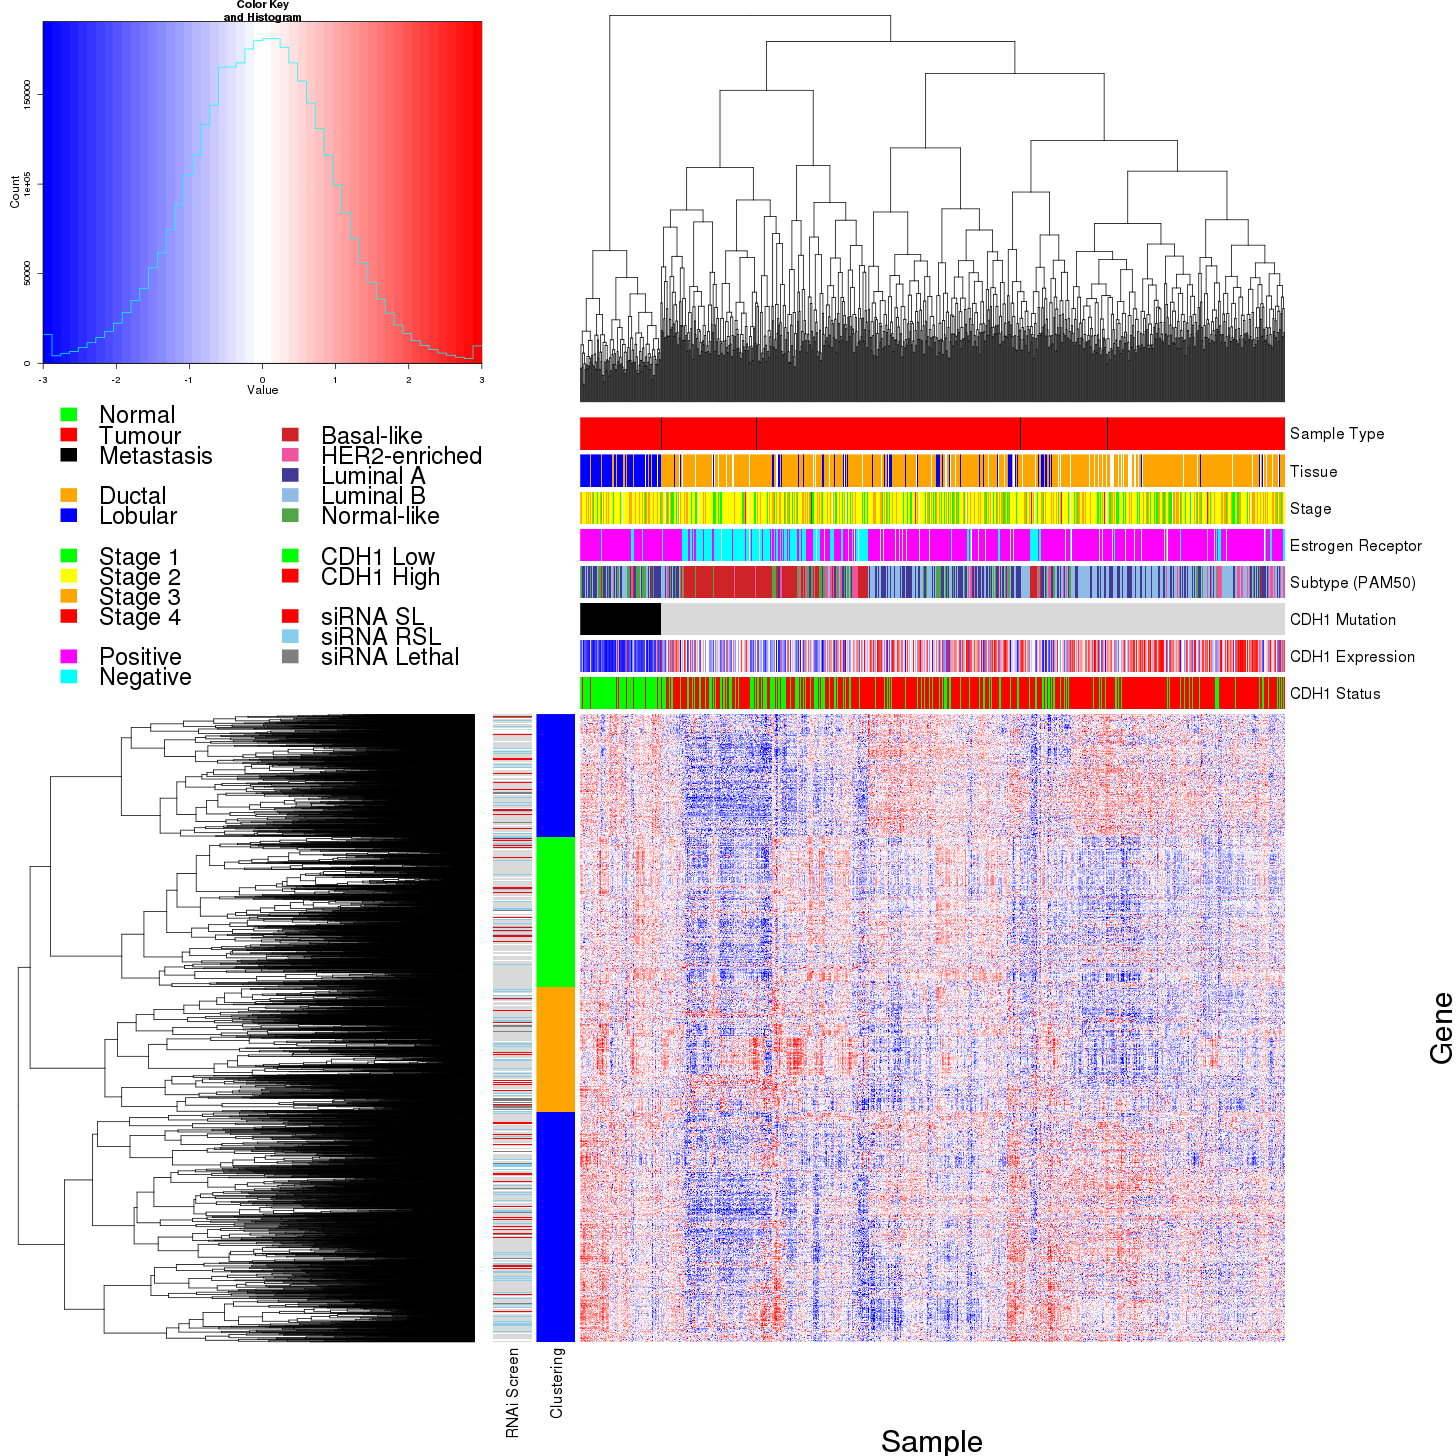
\includegraphics{CDH1_Heatmaps_Genes_Split_By_CDH1_z-trans_mtSL_cordistx_Pub.png}
   }
    \caption[Synthetic lethal expression profiles of analysed samples]{\small \textbf{Synthetic lethal expression profiles of analysed samples.} Gene expression profile heatmap (correlation distance) of all samples (separated by \textit{CDH1} somatic mutation status) analysed in \gls{TCGA} breast cancer dataset for gene expression of 3743 candidate partners of \gls{E-cadherin} (\textit{CDH1}) from \acrshort{mtSLIPT} prediction (with significant \gls{FDR} adjusted $p < 0.05$). Deeply clustered, inter-correlated genes form several main groups, each containing genes that were SL candidates or toxic in an \gls{siRNA} screen \cite{Telford2015}. Clusters had different sample groups highly expressing the synthetic lethal candidates in \textit{CDH1} mutant samples and often lowly expressing \textit{CDH1} wildtype samples (which were not tested for), although many of the \textit{CDH1} mutant samples had among the lowest \textit{CDH1} expression. In contrast to the expression analysis the (predominantly \textit{CDH1} wildtype) basal subtype and \acrshort{ER} negative samples have depleted expression among most candidate synthetic lethal partners. 
   %This suggests that multiple targets may be needed to target \textit{CDH1} deficiency across genetic backgrounds and that combination therapy may be more effective. 
}
\label{fig:slipt_expr_mtSL}
%\end{mdframed}
\end{figure*}

\FloatBarrier


\begin{table*}[!hp]
\caption{Pathways for clusters of \textit{CDH1} partners from mtSLIPT}
\label{tab:pathway_clusters_mtSL}
\centering
%\begin{tiny}
%\makebox[\textwidth][c]{
\resizebox{0.75 \textwidth}{!}{
\begin{threeparttable}
\begin{tabular}{lccc}
%\caption{Pathways for clusters of \textit{CDH1} partners from SLIPT}
%\label{tab:pathway_clusters_mtSL}
  \large{\textbf{Pathways Over-represented in Cluster 1}} & \large{\textbf{Pathway Size}} & \large{\textbf{Cluster Genes}} & \large{\textbf{p-value (\gls{FDR})}} \\ %(833 genes)  
  \hline
  \rowcolor{Cluster_Blue!20}
  Olfactory Signalling Pathway &  57 &   8 & $7.1 \times 10^{-9}$ \\ 
  \rowcolor{Cluster_Blue!15} 
  Assembly of the primary cilium & 149 &  14 & $8.0 \times 10^{-9}$ \\ 
  \rowcolor{Cluster_Blue!20} 
  Sphingolipid metabolism &  62 &   8 & $9.6 \times 10^{-9}$ \\ 
  \rowcolor{Cluster_Blue!15} 
  Signalling by ERBB4 & 133 &  12 & $5.1 \times 10^{-8}$ \\ 
  \rowcolor{Cluster_Blue!20} 
  PI3K Cascade &  65 &   7 & $4.9 \times 10^{-7}$ \\ 
  \rowcolor{Cluster_Blue!15} 
  Circadian Clock &  33 &   5 & $4.9 \times 10^{-7}$ \\ 
  \rowcolor{Cluster_Blue!20} 
  Nuclear signalling by ERBB4 &  34 &   5 & $4.9 \times 10^{-7}$ \\ 
  \rowcolor{Cluster_Blue!15} 
  Intraflagellar transport &  35 &   5 & $4.9 \times 10^{-7}$ \\ 
  \rowcolor{Cluster_Blue!20} 
  PI3K events in ERBB4 signalling &  87 &   8 & $4.9 \times 10^{-7}$ \\ 
  \rowcolor{Cluster_Blue!15} 
  PIP3 activates AKT signalling &  87 &   8 & $4.9 \times 10^{-7}$ \\ 
  \rowcolor{Cluster_Blue!20} 
  PI3K events in ERBB2 signalling &  87 &   8 & $4.9 \times 10^{-7}$ \\ 
  \rowcolor{Cluster_Blue!15} 
  PI-3K cascade:FGFR1 &  87 &   8 & $4.9 \times 10^{-7}$ \\ 
  \rowcolor{Cluster_Blue!20} 
  PI-3K cascade:FGFR2 &  87 &   8 & $4.9 \times 10^{-7}$ \\ 
  \rowcolor{Cluster_Blue!15} 
  PI-3K cascade:FGFR3 &  87 &   8 & $4.9 \times 10^{-7}$ \\ 
  \rowcolor{Cluster_Blue!20} 
  PI-3K cascade:FGFR4 &  87 &   8 & $4.9 \times 10^{-7}$ \\ 
  \rowcolor{Cluster_Blue!15} 
  Deadenylation of \acrshort{mRNA} &  22 &   4 & $5.6 \times 10^{-7}$ \\ 
  \rowcolor{Cluster_Blue!20} 
  PI3K/AKT activation &  90 &   8 & $5.6 \times 10^{-7}$ \\ 
  \rowcolor{Cluster_Blue!15} 
  Cargo trafficking to the periciliary membrane &  38 &   5 & $5.6 \times 10^{-7}$ \\ 
%  \rowcolor{Cluster_Blue!20} 
%  Signalling by Hedgehog & 108 &   9 & $5.6 \times 10^{-7}$ \\ 
%  \rowcolor{Cluster_Blue!15} 
%  Downstream signal transduction & 143 &  11 & $5.6 \times 10^{-7}$ \\ 
  \hline
%  \\
  \cellcolor{white} \large{\textbf{Pathways Over-represented in Cluster 2}} & \large{\textbf{Pathway Size}} & \large{\textbf{Cluster Genes}} & \large{\textbf{p-value (\gls{FDR})}} \\ %(833 genes)  
  \hline
  \rowcolor{Cluster_Green!20}
  G$_{\alpha s}$ signalling events &  83 &  19 & $5.1 \times 10^{-25}$ \\ 
  \rowcolor{Cluster_Green!15}
  Extracellular matrix organization & 238 &  30 & $1.4 \times 10^{-18}$ \\ 
  \rowcolor{Cluster_Green!20} 
  Hemostasis & 422 &  46 & $2.7 \times 10^{-16}$ \\ 
  \rowcolor{Cluster_Green!15} 
  Aquaporin-mediated transport &  32 &   9 & $2.7 \times 10^{-16}$ \\ 
  \rowcolor{Cluster_Green!20} 
  Transcriptional regulation of white adipocyte differentiation &  56 &  11 & $1.7 \times 10^{-15}$ \\ 
  \rowcolor{Cluster_Green!15} 
  Degradation of the extracellular matrix & 102 &  15 & $1.7 \times 10^{-15}$ \\ 
  \rowcolor{Cluster_Green!20} 
  Integration of energy metabolism &  84 &  13 & $8.8 \times 10^{-15}$ \\ 
  \rowcolor{Cluster_Green!15} 
  GPCR downstream signalling & 472 &  48 & $2.8 \times 10^{-14}$ \\ 
  \rowcolor{Cluster_Green!20} 
  G$_{\alpha z}$ signalling events &  15 &   6 & $5.0 \times 10^{-14}$ \\ 
  \rowcolor{Cluster_Green!15} 
  Molecules associated with elastic fibres &  33 &   8 & $5.4 \times 10^{-14}$ \\ 
  \rowcolor{Cluster_Green!20} 
  Phase 1 - Functionalization of compounds &  67 &  11 & $5.6 \times 10^{-14}$ \\ 
  \rowcolor{Cluster_Green!15} 
  Platelet activation, signalling and aggregation & 179 &  20 & $5.6 \times 10^{-14}$ \\ 
  \rowcolor{Cluster_Green!20} 
  Vasopressin regulates renal water homeostasis via Aquaporins &  24 &   7 & $6.1 \times 10^{-14}$ \\ 
  \rowcolor{Cluster_Green!15} 
  Elastic fibre formation &  37 &   8 & $.03 \times 10^{-13}$ \\ 
  \rowcolor{Cluster_Green!20} 
  Calmodulin induced events &  27 &   7 & $3.3 \times 10^{-13}$ \\ 
  \rowcolor{Cluster_Green!15} 
  CaM pathway &  27 &   7 & $3.3 \times 10^{-13}$ \\ 
  \rowcolor{Cluster_Green!20} 
  cGMP effects &  18 &   6 & $3.6 \times 10^{-13}$ \\ 
  \rowcolor{Cluster_Green!15} 
  G$_{\alpha i}$ signalling events & 167 &  18 & $6.3 \times 10^{-13}$ \\ 
%  \rowcolor{Cluster_Green!20} 
%  Ca-dependent events &  29 &   7 & $8.2 \times 10^{-13}$ \\ 
%  \rowcolor{Cluster_Green!15} 
%  Binding and Uptake of Ligands by Scavenger Receptors &  40 &   8 & $8.2 \times 10^{-13}$ \\ 
  \hline
%  \\
  \cellcolor{white} \large{\textbf{Pathways Over-represented in Cluster 3}} & \large{\textbf{Pathway Size}} & \large{\textbf{Cluster Genes}} & \large{\textbf{p-value (\gls{FDR})}} \\ %(833 genes)  
  \hline
  \rowcolor{Cluster_Orange!30}
  Eukaryotic Translation Elongation &  86 &  55 & $1.1 \times 10^{-112}$ \\ 
  \rowcolor{Cluster_Orange!20} 
  Peptide chain elongation &  83 &  54 & $1.3 \times 10^{-112}$ \\ 
  \rowcolor{Cluster_Orange!30} 
  Viral \acrshort{mRNA} Translation &  81 &  53 & $1.6 \times 10^{-111}$ \\ 
  \rowcolor{Cluster_Orange!20} 
  Eukaryotic Translation Termination &  83 &  53 & $7.1 \times 10^{-110}$ \\ 
  \rowcolor{Cluster_Orange!30} 
  Nonsense Mediated Decay independent of the Exon Junction Complex &  88 &  54 & $1.0 \times 10^{-108}$ \\ 
  \rowcolor{Cluster_Orange!20} 
  Formation of a pool of free 40S subunits &  93 &  53 & $4.1 \times 10^{-102}$ \\ 
  \rowcolor{Cluster_Orange!30} 
  Nonsense-Mediated Decay & 103 &  54 & $3.9 \times 10^{-98}$ \\ 
  \rowcolor{Cluster_Orange!20} 
  Nonsense Mediated Decay enhanced by the Exon Junction Complex & 103 &  54 & $3.9 \times 10^{-98}$ \\ 
  \rowcolor{Cluster_Orange!30} 
  L13a-mediated translational silencing of Ceruloplasmin expression & 103 &  53 & $1.2 \times 10^{-95}$ \\ 
  \rowcolor{Cluster_Orange!20} 
  3' -UTR-mediated translational regulation & 103 &  53 & $1.2 \times 10^{-95}$ \\ 
  \rowcolor{Cluster_Orange!30} 
  SRP-dependent cotranslational protein targeting to membrane & 104 &  53 & $4.3 \times 10^{-95}$ \\ 
  \rowcolor{Cluster_Orange!20} 
  GTP hydrolysis and joining of the 60S ribosomal subunit & 104 &  53 & $4.3 \times 10^{-95}$ \\ 
  \rowcolor{Cluster_Orange!30} 
  Influenza Viral \acrshort{RNA} Transcription and Replication & 108 &  53 & $9.6 \times 10^{-93}$ \\ 
  \rowcolor{Cluster_Orange!20} 
  Eukaryotic Translation Initiation & 111 &  53 & $4.2 \times 10^{-91}$ \\ 
  \rowcolor{Cluster_Orange!30} 
  Cap-dependent Translation Initiation & 111 &  53 & $4.2 \times 10^{-91}$ \\ 
  \rowcolor{Cluster_Orange!20} 
  Influenza Life Cycle & 112 &  53 & $1.4 \times 10^{-90}$ \\ 
  \rowcolor{Cluster_Orange!30} 
  Influenza Infection & 117 &  53 & $6.2 \times 10^{-88}$ \\ 
  \rowcolor{Cluster_Orange!20} 
  Translation & 141 &  55 & $3 \times 10^{-81}$ \\ 
%  \rowcolor{Cluster_Orange!30} 
%  Formation of the ternary complex, and subsequently, the 43S complex &  47 &  23 & $2.3 \times 10^{-48}$ \\ 
%  \rowcolor{Cluster_Orange!20} 
%  Translation initiation complex formation &  54 &  23 & $9.1 \times 10^{-45}$ \\ 
  \hline
%  \\ 
  \cellcolor{white} \large{\textbf{Pathways Over-represented in Cluster 4}} & \large{\textbf{Pathway Size}} & \large{\textbf{Cluster Genes}} & \large{\textbf{p-value (\gls{FDR})}} \\ %(833 genes)  
  \hline 
  \rowcolor{Cluster_Red!20}
  ECM proteoglycans &  66 &  10 & $2.9 \times 10^{-11}$ \\ 
  \rowcolor{Cluster_Red!15} 
  deactivation of the beta-catenin transactivating complex &  38 &   7 & $5.1 \times 10^{-10}$ \\ 
  \rowcolor{Cluster_Red!20} 
  Arachidonic acid metabolism &  41 &   7 & $1.1 \times 10^{-9}$ \\ 
  \rowcolor{Cluster_Red!15} 
  G$_{\alpha q}$ signalling events & 149 &  14 & $4.0 \times 10^{-9}$ \\ 
  \rowcolor{Cluster_Red!20} 
  HS-GAG degradation &  21 &   5 & $4.5 \times 10^{-9}$ \\ 
  \rowcolor{Cluster_Red!15} 
  Uptake and actions of bacterial toxins &  22 &   5 & $6.1 \times 10^{-9}$ \\ 
  \rowcolor{Cluster_Red!20} 
  Gastrin-CREB signalling pathway via PKC and MAPK & 170 &  15 & $6.1 \times 10^{-9}$ \\ 
  \rowcolor{Cluster_Red!15} 
  \acrshort{RNA} Polymerase I, \acrshort{RNA} Polymerase III, and Mitochondrial Transcription \textcolor{Cluster_Red!15}{ll}  &  64 &   8 & $6.1 \times 10^{-9}$ \\ 
  \rowcolor{Cluster_Red!20} 
  Non-integrin membrane-ECM interactions &  53 &   7 & $1.5 \times 10^{-8}$ \\ 
  \rowcolor{Cluster_Red!15} 
  Syndecan interactions &  25 &   5 & $1.5 \times 10^{-8}$ \\ 
  \rowcolor{Cluster_Red!20} 
  NOTCH1 Intracellular Domain Regulates Transcription &  40 &   6 & $2.3 \times 10^{-8}$ \\ 
  \rowcolor{Cluster_Red!15} 
  Synthesis of Leukotrienes and Eoxins &  15 &   4 & $3.2 \times 10^{-8}$ \\ 
  \rowcolor{Cluster_Red!20} 
  Signalling by NOTCH1 &  59 &   7 & $5.3 \times 10^{-8}$ \\ 
  \rowcolor{Cluster_Red!15} 
  Regulation of insulin secretion &  44 &   6 & $6.0 \times 10^{-8}$ \\ 
  \rowcolor{Cluster_Red!20} 
  Metabolism of lipids and lipoproteins & 471 &  37 & $8.2 \times 10^{-8}$ \\ 
  \rowcolor{Cluster_Red!15} 
  Signalling by NOTCH &  80 &   8 & $1.2 \times 10^{-7}$ \\ 
  \rowcolor{Cluster_Red!20} 
  Platelet activation, signalling and aggregation & 179 &  14 & $1.2 \times 10^{-7}$ \\ 
  \rowcolor{Cluster_Red!15} 
  Recruitment of mitotic centrosome proteins and complexes &  64 &   7 & $1.2 \times 10^{-7}$ \\ 
%  \rowcolor{Cluster_Red!20} 
%  Centrosome maturation &  64 &   7 & $1.2 \times 10^{-7}$ \\ 
%  \rowcolor{Cluster_Red!15} 
%  Biological oxidations & 133 &  11 & $1.5 \times 10^{-7}$ \\ 
  \hline
\end{tabular}
\begin{tablenotes}
\raggedright %\small
Pathway over-representation analysis for Reactome pathways with the number of genes in each pathway (Pathway Size), number of genes within the pathway identified (Cluster Genes), and the pathway over-representation p-value (adjusted by \gls{FDR}) from the hypergeometric test.  
\end{tablenotes}
\end{threeparttable}
}
\end{table*}


\clearpage
\section{Comparison to Primary Screen}

The mutation synthetic lethal partners with \textit{CDH1} were also compared to \gls{siRNA} primary screen data \citep{Telford2015}, as performed in Section~\ref{chapt3:primary_screen}. These were expected to be more concordant with the experimental results performed on a null mutant, however this was not the case at the gene level: less genes overlapped with experimental candidates in Figure~\ref{fig:Venn_allgenes_mtSL}. This discrepancy was may be due to lower sample size for mutations in \gls{TCGA} data or lower frequency (expected value) of \textit{CDH1} mutations compared to low expression. 

\begin{figure}[!ht]
%\begin{mdframed}
  \centering
  \resizebox{0.66 \columnwidth}{!}{
    \includegraphics{Venn_mtSL_siRNA_allgenes_reduced_Pub.png}
   }
    \caption[Comparison of \acrshort{mtSLIPT} to \gls{siRNA}]{\small \textbf{Comparison of \acrshort{mtSLIPT} to \gls{siRNA}.} Testing the overlap of gene candidates for \gls{E-cadherin} synthetic lethal partners between computational (SLIPT) and experimental screening (siRNA) approaches. The $\chi^2$ test suggests that the overlap is no more than would be expected by chance ($p = 0.281$). %A Venn diagram of all 16298 genes tested by both approaches.
}
\label{fig:Venn_allgenes_mtSL}
%\end{mdframed}
\end{figure}

\FloatBarrier

Despite a lower sample size (and low number of a predicted partners) for mutation analysis, the pathway composition (Tables~\ref{tab:pathway_mtSL} and~\ref{tab:Venn_over-representation_mtSL}) was similar to expression analysis, as described in Section~\ref{chapt3:compare_pathway}. In particular, the resampling analysis (Section~\ref{appendix:compare_pathway_perm_mtSL}) supported many of the results of expression analysis (Section~\ref{chapt3:compare_pathway_perm}). Tables~\ref{tab:pathway_perm_mtSL} and~\ref{tab:pathway_perm_overlap_mtSL} detected many of the same or functionally-related pathways.
 

\begin{table*}[!hp]
\caption{Pathways for \textit{CDH1} partners from \acrshort{mtSLIPT} and \gls{siRNA}}
\label{tab:Venn_over-representation_mtSL}
\centering
\resizebox{0.8 \textwidth}{!}{
\begin{tabular}{sl^c^c^c}
\rowstyle{\bfseries}
  Predicted only by SLIPT (2901 genes) & Pathway Size & Genes Identified & p-value (\gls{FDR}) \\ 
  \hline
  \rowcolor{Cluster_Red!20}
  Eukaryotic Translation Elongation &  87 &  57 & $2.8 \times 10^{-120}$ \\ 
  \rowcolor{Cluster_Red!15}
  Peptide chain elongation &  84 &  56 & $3.1 \times 10^{-120}$ \\ 
  \rowcolor{Cluster_Red!20}
  Eukaryotic Translation Termination &  84 &  55 & $2.8 \times 10^{-117}$ \\ 
  \rowcolor{Cluster_Red!15}
  Viral \acrshort{mRNA} Translation &  82 &  54 & $4.1 \times 10^{-116}$ \\ 
  \rowcolor{Cluster_Red!20}
  Nonsense Mediated Decay independent of the Exon Junction Complex &  89 &  55 & $3.7 \times 10^{-113}$ \\ 
  \rowcolor{Cluster_Red!15}
  Formation of a pool of free 40S subunits &  94 &  55 & $2.8 \times 10^{-109}$ \\ 
  \rowcolor{Cluster_Red!20}
  Nonsense-Mediated Decay & 104 &  57 & $8.4 \times 10^{-108}$ \\ 
  \rowcolor{Cluster_Red!15}
  Nonsense Mediated Decay enhanced by the Exon Junction Complex & 104 &  57 & $8.4 \times 10^{-108}$ \\ 
  \rowcolor{Cluster_Red!20}
  L13a-mediated translational silencing of Ceruloplasmin expression & 104 &  56 & $3.4 \times 10^{-105}$ \\ 
  \rowcolor{Cluster_Red!15}
  3' -UTR-mediated translational regulation & 104 &  56 & $3.4 \times 10^{-105}$ \\ 
  \rowcolor{Cluster_Red!20}
  GTP hydrolysis and joining of the 60S ribosomal subunit & 105 &  56 & $1.4 \times 10^{-104}$ \\ 
  \rowcolor{Cluster_Red!15}
  Eukaryotic Translation Initiation & 112 &  56 & $2.8 \times 10^{-100}$ \\ 
  \rowcolor{Cluster_Red!20}
  Cap-dependent Translation Initiation & 112 &  56 & $2.8 \times 10^{-100}$ \\ 
  \rowcolor{Cluster_Red!15}
  SRP-dependent cotranslational protein targeting to membrane & 105 &  54 & $2.2 \times 10^{-99}$ \\ 
  \rowcolor{Cluster_Red!20}
  Influenza Viral \acrshort{RNA} Transcription and Replication & 109 &  54 & $5.3 \times 10^{-97}$ \\ 
  \rowcolor{Cluster_Red!15}
  Influenza Life Cycle & 113 &  54 & $9.6 \times 10^{-95}$ \\ 
  \rowcolor{Cluster_Red!20}
  Influenza Infection & 118 &  55 & $1.7 \times 10^{-94}$ \\ 
  \rowcolor{Cluster_Red!15}
  Translation & 142 &  60 & $3.5 \times 10^{-94}$ \\ 
  \rowcolor{Cluster_Red!20}
  Infectious disease & 349 &  77 & $5.9 \times 10^{-62}$ \\ 
  \rowcolor{Cluster_Red!15}
  Extracellular matrix organization & 241 &  54 & $3.0 \times 10^{-52}$ \\
  \hline
  \\
  \rowstyle{\bfseries}
  Detected only by \gls{siRNA} screen (1752 genes) & Pathway Size & Genes Identified & p-value (\gls{FDR}) \\ 
  \hline
  \rowcolor{Cluster_Blue!20}
  Class A/1 (Rhodopsin-like receptors) & 282 &  69 & $1.9 \times 10^{-59}$ \\ 
  \rowcolor{Cluster_Blue!15}
  GPCR ligand binding & 363 &  78 & $2.7 \times 10^{-54}$ \\ 
  \rowcolor{Cluster_Blue!20}
  Peptide ligand-binding receptors & 175 &  41 & $1.5 \times 10^{-42}$ \\ 
  \rowcolor{Cluster_Blue!15}
  $G_{\alpha i}$ signalling events & 184 &  41 & $1.1 \times 10^{-40}$ \\ 
  \rowcolor{Cluster_Blue!20}
  Gastrin-CREB signalling pathway via PKC and MAPK & 180 &  37 & $1.5 \times 10^{-35}$ \\ 
  \rowcolor{Cluster_Blue!15}
  $G_{\alpha q}$ signalling events & 159 &  34 & $3.7 \times 10^{-35}$ \\ 
  \rowcolor{Cluster_Blue!20}
  DAP12 interactions & 159 &  27 & $1.1 \times 10^{-24}$ \\ 
  \rowcolor{Cluster_Blue!15}
  VEGFA-VEGFR2 Pathway &  91 &  19 & $1.0 \times 10^{-23}$ \\ 
  \rowcolor{Cluster_Blue!20}
  Downstream signal transduction & 146 &  24 & $1.9 \times 10^{-22}$ \\ 
  \rowcolor{Cluster_Blue!15}
  Signalling by VEGF &  99 &  19 & $2.6 \times 10^{-22}$ \\ 
  \rowcolor{Cluster_Blue!20}
  DAP12 signalling & 149 &  24 & $4.2 \times 10^{-22}$ \\ 
  \rowcolor{Cluster_Blue!15}
  Organelle biogenesis and maintenance & 264 &  34 & $4.3 \times 10^{-20}$ \\ 
  \rowcolor{Cluster_Blue!20}
  Downstream signalling of activated FGFR1 & 134 &  21 & $4.3 \times 10^{-20}$ \\ 
  \rowcolor{Cluster_Blue!15}
  Downstream signalling of activated FGFR2 & 134 &  21 & $4.3 \times 10^{-20}$ \\ 
  \rowcolor{Cluster_Blue!20}
  Downstream signalling of activated FGFR3 & 134 &  21 & $4.3 \times 10^{-20}$ \\ 
  \rowcolor{Cluster_Blue!15}
  Downstream signalling of activated FGFR4 & 134 &  21 & $4.3 \times 10^{-20}$ \\ 
  \rowcolor{Cluster_Blue!20}
  Signalling by ERBB2 & 146 &  22 & $5.3 \times 10^{-20}$ \\ 
  \rowcolor{Cluster_Blue!15}
  Signalling by FGFR & 146 &  22 & $5.3 \times 10^{-20}$ \\ 
  \rowcolor{Cluster_Blue!20}
  Signalling by FGFR1 & 146 &  22 & $5.3 \times 10^{-20}$ \\ 
  \rowcolor{Cluster_Blue!15}
  Signalling by FGFR2 & 146 &  22 & $5.3 \times 10^{-20}$ \\ 
  \hline
  \\
  \rowstyle{\bfseries}
  Intersection of SLIPT and \gls{siRNA} screen (450 genes) & Pathway Size & Genes Identified & p-value (\gls{FDR}) \\ 
  \hline
  \rowcolor{Cluster_Red!20!Cluster_Blue!20}
  HS-GAG degradation &  21 &   4 & $4.9 \times 10^{-6}$ \\ 
  \rowcolor{Cluster_Red!15!Cluster_Blue!15}
  Retinoid metabolism and transport &  39 &   5 & $4.9 \times 10^{-6}$ \\ 
  \rowcolor{Cluster_Red!20!Cluster_Blue!20}
  Platelet activation, signalling and aggregation & 186 &  13 & $4.9 \times 10^{-6}$ \\ 
  \rowcolor{Cluster_Red!15!Cluster_Blue!15}
  Signalling by NOTCH4 &  11 &   3 & $4.9 \times 10^{-6}$ \\ 
  \rowcolor{Cluster_Red!20!Cluster_Blue!20}
  $G_{\alpha s}$ signalling events & 100 &   8 & $5.0 \times 10^{-6}$ \\ 
  \rowcolor{Cluster_Red!15!Cluster_Blue!15}
  Defective EXT2 causes exostoses 2 &  12 &   3 & $5.0 \times 10^{-6}$ \\ 
  \rowcolor{Cluster_Red!20!Cluster_Blue!20}
  Defective EXT1 causes exostoses 1, TRPS2 and CHDS &  12 &   3 & $5.0 \times 10^{-6}$ \\ 
  \rowcolor{Cluster_Red!15!Cluster_Blue!15}
  Class A/1 (Rhodopsin-like receptors) & 289 &  18 & $2.2 \times 10^{-5}$ \\ 
  \rowcolor{Cluster_Red!20!Cluster_Blue!20}
  Signalling by PDGF & 173 &  11 & $2.9 \times 10^{-5}$ \\ 
  \rowcolor{Cluster_Red!15!Cluster_Blue!15}
  Circadian Clock &  34 &   4 & $2.9 \times 10^{-5}$ \\ 
  \rowcolor{Cluster_Red!20!Cluster_Blue!20}
  Signalling by ERBB4 & 139 &   9 & $4.3 \times 10^{-5}$ \\ 
  \rowcolor{Cluster_Red!15!Cluster_Blue!15}
  Role of LAT2/NTAL/LAB on calcium mobilization &  99 &   7 & $4.4 \times 10^{-5}$ \\ 
  \rowcolor{Cluster_Red!20!Cluster_Blue!20}
  Peptide ligand-binding receptors & 181 &  11 & $4.5 \times 10^{-5}$ \\ 
  \rowcolor{Cluster_Red!15!Cluster_Blue!15}
  Defective B4GALT7 causes EDS, progeroid type &  19 &   3 & $4.5 \times 10^{-5}$ \\ 
  \rowcolor{Cluster_Red!20!Cluster_Blue!20}
  Defective B3GAT3 causes JDSSDHD &  19 &   3 & $4.5 \times 10^{-5}$ \\ 
  \rowcolor{Cluster_Red!15!Cluster_Blue!15}
  Signalling by NOTCH &  80 &   6 & $4.5 \times 10^{-5}$ \\ 
  \rowcolor{Cluster_Red!20!Cluster_Blue!20}
  $G_{\alpha q}$ signalling events & 164 &  10 & $5.1 \times 10^{-5}$ \\ 
  \rowcolor{Cluster_Red!15!Cluster_Blue!15}
  Response to elevated platelet cytosolic Ca$^{2+}$ &  84 &   6 & $7.1 \times 10^{-5}$ \\ 
  \rowcolor{Cluster_Red!20!Cluster_Blue!20}
  Signalling by ERBB2 & 148 &   9 & $7.1 \times 10^{-5}$ \\ 
  \rowcolor{Cluster_Red!15!Cluster_Blue!15}
  Signalling by SCF-KIT & 129 &   8 & $8.3 \times 10^{-5}$ \\ 
  \hline
\end{tabular}
}
\end{table*}


\clearpage
\subsection{Resampling Analysis}  \label{appendix:compare_pathway_perm_mtSL}

\begin{table*}[!htp]
\caption{Pathways for \textit{CDH1} partners from mtSLIPT}
\label{tab:pathway_perm_mtSL}
\centering
\resizebox{0.8 \textwidth}{!}{
\begin{threeparttable}
\begin{tabular}{sl^c^c}
\rowstyle{\bfseries}
 Reactome Pathway & Over-representation & Permutation \\ 
  \hline
  \rowcolor{Cluster_Red!20} 
  \textbf{Eukaryotic Translation Elongation} & $3.2 \times 10^{-128}$ & $<7.035 \times 10^{-4}$ \\ 
    \rowcolor{Cluster_Red!15} 
  \textbf{Peptide chain elongation} & $3.2 \times 10^{-128}$ & $<7.035 \times 10^{-4}$ \\ 
    \rowcolor{Cluster_Red!20} 
  \textbf{Eukaryotic Translation Termination} & $3.7 \times 10^{-125}$ & $<7.035 \times 10^{-4}$ \\ 
    \rowcolor{Cluster_Red!15} 
  \textbf{Viral \acrshort{mRNA} Translation} & $4.1 \times 10^{-124}$ & $<7.035 \times 10^{-4}$ \\ 
    \rowcolor{Cluster_Red!20} 
  \textbf{Nonsense Mediated Decay independent of the Exon Junction Complex} & $1.4 \times 10^{-123}$ & $<7.035 \times 10^{-4}$ \\ 
    \rowcolor{Cluster_Red!15} 
  \textbf{Nonsense-Mediated Decay} & $8.4 \times 10^{-117}$ & $<7.035 \times 10^{-4}$ \\ 
    \rowcolor{Cluster_Red!20} 
  \textbf{Nonsense Mediated Decay enhanced by the Exon Junction Complex} & $8.4 \times 10^{-117}$ & $<7.035 \times 10^{-4}$ \\ 
    \rowcolor{Cluster_Red!15} 
  \textbf{Formation of a pool of free 40S subunits} & $2.6 \times 10^{-116}$ & $<7.035 \times 10^{-4}$ \\ 
    \rowcolor{Cluster_Red!20} 
  \textbf{L13a-mediated translational silencing of Ceruloplasmin expression} & $2.0 \times 10^{-111}$ & $<7.035 \times 10^{-4}$ \\ 
    \rowcolor{Cluster_Red!15} 
  \textbf{3' -UTR-mediated translational regulation} & $2.0 \times 10^{-111}$ & $<7.035 \times 10^{-4}$ \\ 
    \rowcolor{Cluster_Red!20} 
  \textbf{GTP hydrolysis and joining of the 60S ribosomal subunit} & $9.9 \times 10^{-111}$ & $<7.035 \times 10^{-4}$ \\ 
    \rowcolor{Cluster_Red!15} 
 \textbf{SRP-dependent cotranslational protein targeting to membrane} & $4.7 \times 10^{-108}$ & $<7.035 \times 10^{-4}$ \\ 
    \rowcolor{Cluster_Red!20} 
  \textbf{Eukaryotic Translation Initiation} & $4.8 \times 10^{-106}$ & $<7.035 \times 10^{-4}$ \\ 
    \rowcolor{Cluster_Red!15} 
  \textbf{Cap-dependent Translation Initiation} & $4.8 \times 10^{-106}$ & $<7.035 \times 10^{-4}$ \\ 
    \rowcolor{Cluster_Red!20} 
  \textbf{Influenza Viral \acrshort{RNA} Transcription and Replication} & $8.1 \times 10^{-103}$ & $<7.035 \times 10^{-4}$ \\ 
    \rowcolor{Cluster_Red!15} 
  \textbf{Influenza Infection} & $2.4 \times 10^{-102}$ & $<7.035 \times 10^{-4}$ \\ 
    \rowcolor{Cluster_Red!20} 
  \textbf{Translation} & $6.0 \times 10^{-101}$ & $<7.035 \times 10^{-4}$ \\ 
    \rowcolor{Cluster_Red!15} 
  \textbf{Influenza Life Cycle} & $2.2 \times 10^{-100}$ & $<7.035 \times 10^{-4}$ \\ 
    \rowcolor{Cluster_Red!20} 
  \textbf{Disease} & $2.1 \times 10^{-90}$ & $0.013347$ \\ 
    \rowcolor{Cluster_Red!15} 
  \textbf{GPCR downstream signalling} & $1.6 \times 10^{-80}$ & $0.095478$ \\ 
    \rowcolor{Cluster_Red!20} 
  Hemostasis & $2.1 \times 10^{-78}$ & $0.2671$ \\ 
    \rowcolor{Cluster_Red!15} 
  Signalling by GPCR & $1.2 \times 10^{-73}$ & $0.44939$ \\ 
    \rowcolor{Cluster_Red!20} 
  \textit{Extracellular matrix organization} & $2.2 \times 10^{-67}$ & $0.054008$ \\ 
    \rowcolor{Cluster_Red!15} 
  Metabolism of proteins & $1.4 \times 10^{-66}$ & $0.9607$ \\ 
    \rowcolor{Cluster_Red!20} 
  Signal Transduction & $2.1 \times 10^{-66}$ & $0.48184$ \\ 
    \rowcolor{Cluster_Red!15} 
  Developmental Biology & $2.5 \times 10^{-66}$ & $0.54075$ \\ 
    \rowcolor{Cluster_Red!20} 
  Innate Immune System & $5.3 \times 10^{-66}$ & $0.9589$ \\ 
    \rowcolor{Cluster_Red!15} 
  Infectious disease & $9.6 \times 10^{-66}$ & $0.21075$ \\ 
    \rowcolor{Cluster_Red!20} 
  Signalling by NGF & $1.1 \times 10^{-62}$ & $0.43356$ \\ 
    \rowcolor{Cluster_Red!15} 
  Immune System & $2.8 \times 10^{-62}$ & $0.23052$ \\ 
  \iffalse
  \rowcolor{Cluster_Red!20} 
    Metabolism of lipids and lipoproteins & $6.4 \times 10^{-58}$ & $0.72543$ \\ 
    \rowcolor{Cluster_Red!15} 
  Metabolism & $9.7 \times 10^{-56}$ & $0.72543$ \\ 
    \rowcolor{Cluster_Red!20} 
  Platelet activation, signalling and aggregation & $3.4 \times 10^{-55}$ & $0.29119$ \\ 
    \rowcolor{Cluster_Red!15} 
  GPCR ligand binding & $9.3 \times 10^{-55}$ & $0.59136$ \\ 
    \rowcolor{Cluster_Red!20} 
  Signalling by PDGF & $1.1 \times 10^{-54}$ & $0.40041$ \\ 
    \rowcolor{Cluster_Red!15} 
  Class A/1 (Rhodopsin-like receptors) & $4.2 \times 10^{-54}$ & $0.63215$ \\ 
    \rowcolor{Cluster_Red!20} 
  Fc epsilon receptor (FCERI) signalling & $8 \times 10^{-53}$ & $0.44441$ \\ 
    \rowcolor{Cluster_Red!15} 
  Adaptive Immune System & $6.7 \times 10^{-52}$ & $0.14054$ \\ 
    \rowcolor{Cluster_Red!20} 
  Signalling by ERBB4 & $7.8 \times 10^{-52}$ & $0.24354$ \\ 
    \rowcolor{Cluster_Red!15} 
  Axon guidance & $1.2 \times 10^{-51}$ & $0.6903$ \\ 
    \rowcolor{Cluster_Red!20} 
  Formation of the ternary complex, and subsequently, the 43S complex & $2.2 \times 10^{-51}$ & $<7.035 \times 10^{-4}$ \\ 
    \rowcolor{Cluster_Red!15} 
  Translation initiation complex formation & $3 \times 10^{-50}$ & $<7.035 \times 10^{-4}$ \\ 
    \rowcolor{Cluster_Red!20} 
  Ribosomal scanning and start codon recognition & $3 \times 10^{-50}$ & $<7.035 \times 10^{-4}$ \\ 
    \rowcolor{Cluster_Red!15} 
  NGF signalling via TRKA from the plasma membrane & $9.1 \times 10^{-50}$ & $0.60808$ \\ 
    \rowcolor{Cluster_Red!20} 
  \begin{tabular}[c]{@{}l@{}}Activation of the \acrshort{mRNA} upon binding of the cap-binding complex and eIFs,\\and subsequent binding to 43S \end{tabular} & $9.6 \times 10^{-50}$ & $<7.035 \times 10^{-4}$ \\ 
    \rowcolor{Cluster_Red!15} 
  Transmembrane transport of small molecules & $2.5 \times 10^{-49}$ & $0.17506$ \\ 
    \rowcolor{Cluster_Red!20} 
  Signalling by ERBB2 & $8.1 \times 10^{-49}$ & $0.45422$ \\ 
    \rowcolor{Cluster_Red!15} 
  Rho GTPase cycle & $4.9 \times 10^{-48}$ & $0.10613$ \\ 
    \rowcolor{Cluster_Red!20} 
  G$_{\alpha s}$ signalling events & $1.5 \times 10^{-47}$ & $0.0026835$ \\ 
    \rowcolor{Cluster_Red!15} 
  Signalling by FGFR & $2.4 \times 10^{-47}$ & $0.54308$ \\ 
  \fi
  \hline
\end{tabular}
\begin{tablenotes}
\raggedright \small
Over-representation (hypergeometric test) and Permutation p-values adjusted for multiple tests across pathways (\gls{FDR}). Significant pathways were marked in bold (\gls{FDR} $ < 0.05$) and italics (\gls{FDR} $ < 0.1$).
\end{tablenotes}
\end{threeparttable}
}
\end{table*}


\begin{table*}[!htp]
\caption{Pathways for \textit{CDH1} partners from \acrshort{mtSLIPT} and \gls{siRNA} primary screen}
\label{tab:pathway_perm_overlap_mtSL}
\centering
\resizebox{0.8 \textwidth}{!}{
\begin{threeparttable}
\begin{tabular}{sl^c^c}
\rowstyle{\bfseries}
 Reactome Pathway & Over-representation & Permutation \\ 
  \hline
  \rowcolor{Cluster_Red!20!Cluster_Blue!20} 
  Visual phototransduction & $1.2 \times 10^{-9}$ & $0.86279$ \\ 
    \rowcolor{Cluster_Red!15!Cluster_Blue!15} 
  \textbf{G$_{\alpha s}$ signalling events} & $2.9 \times 10^{-7}$ & $0.023066$ \\ 
    \rowcolor{Cluster_Red!20!Cluster_Blue!20} 
  Retinoid metabolism and transport & $2.9 \times 10^{-7}$ & $0.299$ \\ 
    \rowcolor{Cluster_Red!15!Cluster_Blue!15} 
  Acyl chain remodelling of PS & $1.1 \times 10^{-5}$ & $0.42584$ \\ 
    \rowcolor{Cluster_Red!20!Cluster_Blue!20} 
  Transcriptional regulation of white adipocyte differentiation & $1.1 \times 10^{-5}$ & $0.53928$ \\ 
    \rowcolor{Cluster_Red!15!Cluster_Blue!15} 
  Chemokine receptors bind chemokines & $1.1 \times 10^{-5}$ & $0.95259$ \\ 
    \rowcolor{Cluster_Red!20!Cluster_Blue!20} 
  \textit{Signalling by NOTCH4} & $1.2 \times 10^{-5}$ & $0.079229$ \\ 
    \rowcolor{Cluster_Red!15!Cluster_Blue!15} 
  Defective EXT2 causes exostoses 2 & $1.2 \times 10^{-5}$ & $0.22292$ \\ 
    \rowcolor{Cluster_Red!20!Cluster_Blue!20} 
  Defective EXT1 causes exostoses 1, TRPS2 and CHDS & $1.2 \times 10^{-5}$ & $0.22292$ \\ 
    \rowcolor{Cluster_Red!15!Cluster_Blue!15} 
  Platelet activation, signalling and aggregation & $1.2 \times 10^{-5}$ & $0.48853$ \\ 
    \rowcolor{Cluster_Red!20!Cluster_Blue!20} 
  Serotonin receptors & $1.4 \times 10^{-5}$ & $0.34596$ \\ 
    \rowcolor{Cluster_Red!15!Cluster_Blue!15} 
  Nicotinamide salvaging & $1.4 \times 10^{-5}$ & $0.70881$ \\ 
    \rowcolor{Cluster_Red!20!Cluster_Blue!20} 
  Phase 1 - Functionalization of compounds & $2 \times 10^{-5}$ & $0.31142$ \\ 
    \rowcolor{Cluster_Red!15!Cluster_Blue!15} 
  Amine ligand-binding receptors & $2.5 \times 10^{-5}$ & $0.34934$ \\ 
    \rowcolor{Cluster_Red!20!Cluster_Blue!20} 
  Acyl chain remodelling of PE & $3.8 \times 10^{-5}$ & $0.42615$ \\ 
    \rowcolor{Cluster_Red!15!Cluster_Blue!15} 
  Signalling by GPCR & $3.8 \times 10^{-5}$ & $0.93888$ \\ 
    \rowcolor{Cluster_Red!20!Cluster_Blue!20} 
  \textbf{Molecules associated with elastic fibres} & $3.9 \times 10^{-5}$ & $0.017982$ \\ 
    \rowcolor{Cluster_Red!15!Cluster_Blue!15} 
  DAP12 interactions & $3.9 \times 10^{-5}$ & $0.71983$ \\ 
    \rowcolor{Cluster_Red!20!Cluster_Blue!20} 
  Beta defensins & $3.9 \times 10^{-5}$ & $0.91458$ \\ 
    \rowcolor{Cluster_Red!15!Cluster_Blue!15} 
  Cytochrome P$_{450}$ - arranged by substrate type & $4.7 \times 10^{-5}$ & $0.83493$ \\ 
    \rowcolor{Cluster_Red!20!Cluster_Blue!20} 
  GPCR ligand binding & $5.7 \times 10^{-5}$ & $0.95258$ \\ 
    \rowcolor{Cluster_Red!15!Cluster_Blue!15} 
  Acyl chain remodelling of PC & $6.1 \times 10^{-5}$ & $0.42584$ \\ 
    \rowcolor{Cluster_Red!20!Cluster_Blue!20} 
  Response to elevated platelet cytosolic Ca$^{2+}$ & $6.4 \times 10^{-5}$ & $0.54046$ \\ 
    \rowcolor{Cluster_Red!15!Cluster_Blue!15} 
  \textbf{Arachidonic acid metabolism} & $6.7 \times 10^{-5}$ & $0.026696$ \\ 
    \rowcolor{Cluster_Red!20!Cluster_Blue!20} 
  Defective B4GALT7 causes EDS, progeroid type & $7.3 \times 10^{-5}$ & $0.24921$ \\ 
    \rowcolor{Cluster_Red!15!Cluster_Blue!15} 
  Defective B3GAT3 causes JDSSDHD & $7.3 \times 10^{-5}$ & $0.24921$ \\ 
    \rowcolor{Cluster_Red!20!Cluster_Blue!20} 
  Hydrolysis of LPC & $7.3 \times 10^{-5}$ & $0.80663$ \\ 
    \rowcolor{Cluster_Red!15!Cluster_Blue!15} 
  \textbf{Elastic fibre formation} & $7.4 \times 10^{-5}$ & $0.0058768$ \\ 
    \rowcolor{Cluster_Red!20!Cluster_Blue!20} 
 \textbf{ HS-GAG degradation} & $9.4 \times 10^{-5}$ & $0.0083179$ \\ 
    \rowcolor{Cluster_Red!15!Cluster_Blue!15} 
  \textit{Bile acid and bile salt metabolism} & $9.4 \times 10^{-5}$ & $0.079905$ \\ 
    \rowcolor{Cluster_Red!20!Cluster_Blue!20} 
  Netrin-1 signalling & $0.00011$ & $0.92216$ \\ 
    \rowcolor{Cluster_Red!15!Cluster_Blue!15} 
  \textbf{Integration of energy metabolism} & $0.00011$ & $0.011152$ \\ 
    \rowcolor{Cluster_Red!20!Cluster_Blue!20} 
  Dectin-2 family & $0.00012$ & $0.10385$ \\ 
    \rowcolor{Cluster_Red!15!Cluster_Blue!15} 
  Platelet sensitization by LDL & $0.00012$ & $0.34596$ \\ 
    \rowcolor{Cluster_Red!20!Cluster_Blue!20} 
  DAP12 signalling & $0.00012$ & $0.62787$ \\ 
    \rowcolor{Cluster_Red!15!Cluster_Blue!15} 
  Defensins & $0.00012$ & $0.77542$ \\ 
    \rowcolor{Cluster_Red!20!Cluster_Blue!20} 
  GPCR downstream signalling & $0.00012$ & $0.79454$ \\ 
    \rowcolor{Cluster_Red!15!Cluster_Blue!15} 
  \textit{Diseases associated with glycosaminoglycan metabolism} & $0.00013$ & $0.065927$ \\ 
    \rowcolor{Cluster_Red!20!Cluster_Blue!20} 
  \textit{Diseases of glycosylation} & $0.00013$ & $0.065927$ \\ 
    \rowcolor{Cluster_Red!15!Cluster_Blue!15} 
  Signalling by Retinoic Acid & $0.00013$ & $0.22292$ \\ 
    \rowcolor{Cluster_Red!20!Cluster_Blue!20} 
  Signalling by Leptin & $0.00013$ & $0.34596$ \\ 
    \rowcolor{Cluster_Red!15!Cluster_Blue!15} 
  Signalling by SCF-KIT & $0.00013$ & $0.70881$ \\ 
    \rowcolor{Cluster_Red!20!Cluster_Blue!20} 
  Opioid Signalling & $0.00013$ & $0.96053$ \\ 
    \rowcolor{Cluster_Red!15!Cluster_Blue!15} 
  Signalling by NOTCH & $0.00015$ & $0.26884$ \\ 
    \rowcolor{Cluster_Red!20!Cluster_Blue!20} 
  Platelet homeostasis & $0.00015$ & $0.4878$ \\ 
    \rowcolor{Cluster_Red!15!Cluster_Blue!15} 
  Signalling by NOTCH1 & $0.00016$ & $0.13043$ \\ 
    \rowcolor{Cluster_Red!20!Cluster_Blue!20} 
  Class B/2 (Secretin family receptors) & $0.00016$ & $0.13994$ \\ 
    \rowcolor{Cluster_Red!15!Cluster_Blue!15} 
  \textit{Diseases of Immune System} & $0.0002$ & $0.0795$ \\ 
    \rowcolor{Cluster_Red!20!Cluster_Blue!20} 
  \textit{Diseases associated with the TLR signalling cascade} & $0.0002$ & $0.0795$ \\ 
    \rowcolor{Cluster_Red!15!Cluster_Blue!15} 
  A tetrasaccharide linker sequence is required for GAG synthesis & $0.0002$ & $0.42615$ \\
  \hline
\end{tabular}
\begin{tablenotes}
\raggedright \small
Over-representation (hypergeometric test) and Permutation p-values adjusted for multiple tests across pathways (\gls{FDR}). Significant pathways were marked in bold (\gls{FDR} $ < 0.05$) and italics (\gls{FDR} $ < 0.1$).
\end{tablenotes}
\end{threeparttable}
}
\end{table*}

\iffalse
\begin{table}
\caption{Pathways for \textit{CDH1} partners from \acrshort{mtSLIPT} and \gls{siRNA} screen}
\label{tab:pathway_perm_overlap_small_mtSL}
\centering
\resizebox{1 \textwidth}{!}{
\begin{tabular}{sl^c^c}
\rowstyle{\bfseries}
Reactome Pathway & Over-representation & Permutation \\ 
  \hline
  \rowcolor{Cluster_Red!20!Cluster_Blue!20} 
  \textbf{G$_{\alpha s}$ signalling events} & $3.305 \times 10^{-7}$ & $2.229 \times 10^{-2}$ \\
  \rowcolor{Cluster_Red!15!Cluster_Blue!15}  
  \textit{Signalling by NOTCH4} & $1.642 \times 10^{-5}$ & $7.159 \times 10^{-2}$ \\
  \rowcolor{Cluster_Red!20!Cluster_Blue!20}  
  Defective EXT2 causes exostoses 2 & $1.642 \times 10^{-5}$ & $1.880 \times 10^{-1}$ \\
  \rowcolor{Cluster_Red!15!Cluster_Blue!15}  
  Defective EXT1 causes exostoses 1, TRPS2 and CHDS & $1.642 \times 10^{-5}$ & $1.880 \times 10^{-1}$ \\
  \rowcolor{Cluster_Red!20!Cluster_Blue!20}  
  Retinoid metabolism and transport & $1.642 \times 10^{-5}$ & $2.587 \times 10^{-1}$ \\
  \rowcolor{Cluster_Red!15!Cluster_Blue!15}  
  \textbf{Circadian Clock} & $1.405 \times 10^{-4}$ & $2.229 \times 10^{-2}$ \\
  \rowcolor{Cluster_Red!20!Cluster_Blue!20}  
  Defective B4GALT7 causes EDS, progeroid type & $1.405 \times 10^{-4}$ & $2.071 \times 10^{-1}$ \\
  \rowcolor{Cluster_Red!15!Cluster_Blue!15}  
  Defective B3GAT3 causes JDSSDHD & $1.405 \times 10^{-4}$ & $2.071 \times 10^{-1}$ \\
  \rowcolor{Cluster_Red!20!Cluster_Blue!20}  
  \textbf{HS-GAG degradation} & $1.795 \times 10^{-4}$ & $6.056 \times 10^{-3}$ \\
  \rowcolor{Cluster_Red!15!Cluster_Blue!15}  
  \textit{Growth hormone receptor signalling} & $2.274 \times 10^{-4}$ & $7.127 \times 10^{-2}$ \\
  \rowcolor{Cluster_Red!20!Cluster_Blue!20}  
  \textit{Diseases associated with glycosaminoglycan metabolism} & $2.618 \times 10^{-4}$ & $6.388 \times 10^{-2}$ \\
  \hline
\end{tabular}
}
\end{table}
\fi

\clearpage
\section{Compare \gls{SLIPT} genes} \label{appendix:compare_mtSL}

The mutation synthetic lethal partners with \textit{CDH1} were also compared to \gls{siRNA} primary screen data \citep{Telford2015}, by correlation and \gls{siRNA} viability as described in sections~\ref{chapt3:compare_correlation} and~\ref{chapt3:compare_viability}.

\begin{figure*}[!htp]
%\begin{mdframed}
\begin{center}
  \resizebox{0.75 \textwidth}{!}{
    \includegraphics{mtSLIPT_siRNA_vs_Correlation_with_CDH1.png}
   }
   \end{center}
   \caption[Compare \acrshort{mtSLIPT} and \gls{siRNA} genes with correlation]{\small \textbf{Compare \acrshort{mtSLIPT} and \gls{siRNA} genes with correlation.} The \acrshort{mtSLIPT} p-values were compared against Pearson's correlation of expression with \textit{CDH1}. Genes detected by SLIPT or \gls{siRNA} were coloured according to the legend. 
}
\label{fig:compare_points_correlation_mtSL}
%\end{mdframed}
%\end{figure*}

%\begin{figure*}[!htp]
%\begin{mdframed}
\begin{center}
  \resizebox{0.75 \textwidth}{!}{
    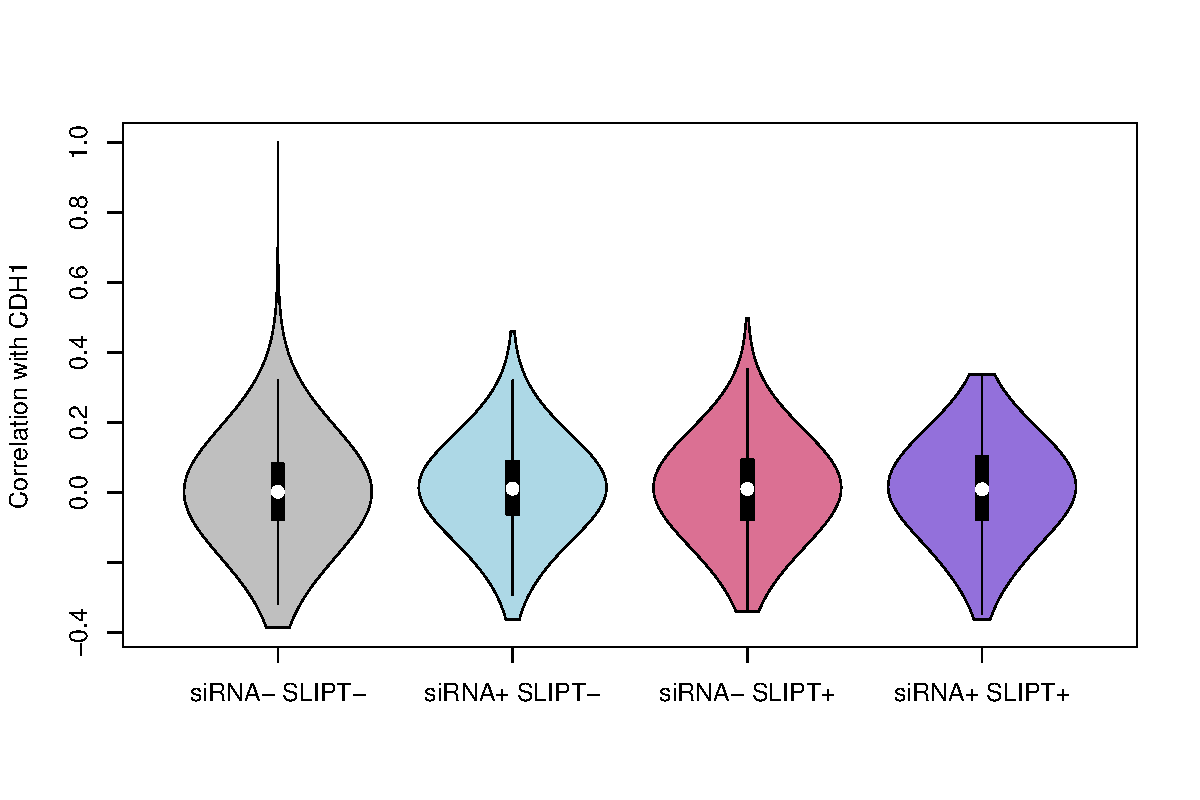
\includegraphics{vioplotx_mtSLIPT_siRNA_vs_CDH1_Correlation_with_CDH1.pdf}
   }
   \end{center}
   \caption[Compare \acrshort{mtSLIPT} and \gls{siRNA} genes with correlation]{\small \textbf{Compare \acrshort{mtSLIPT} and \gls{siRNA} genes with correlation.}  Genes detected by \acrshort{mtSLIPT} against \textit{CDH1} mutation and \gls{siRNA} screening were compared against Pearson's correlation of expression with \textit{CDH1}. There were no differences in correlation between the gene groups. 
}
\label{fig:compare_correlation_mtSL}
%\end{mdframed}
\end{figure*}

\begin{figure*}[!htp]
%\begin{mdframed}
\begin{center}
  \resizebox{0.75 \textwidth}{!}{
    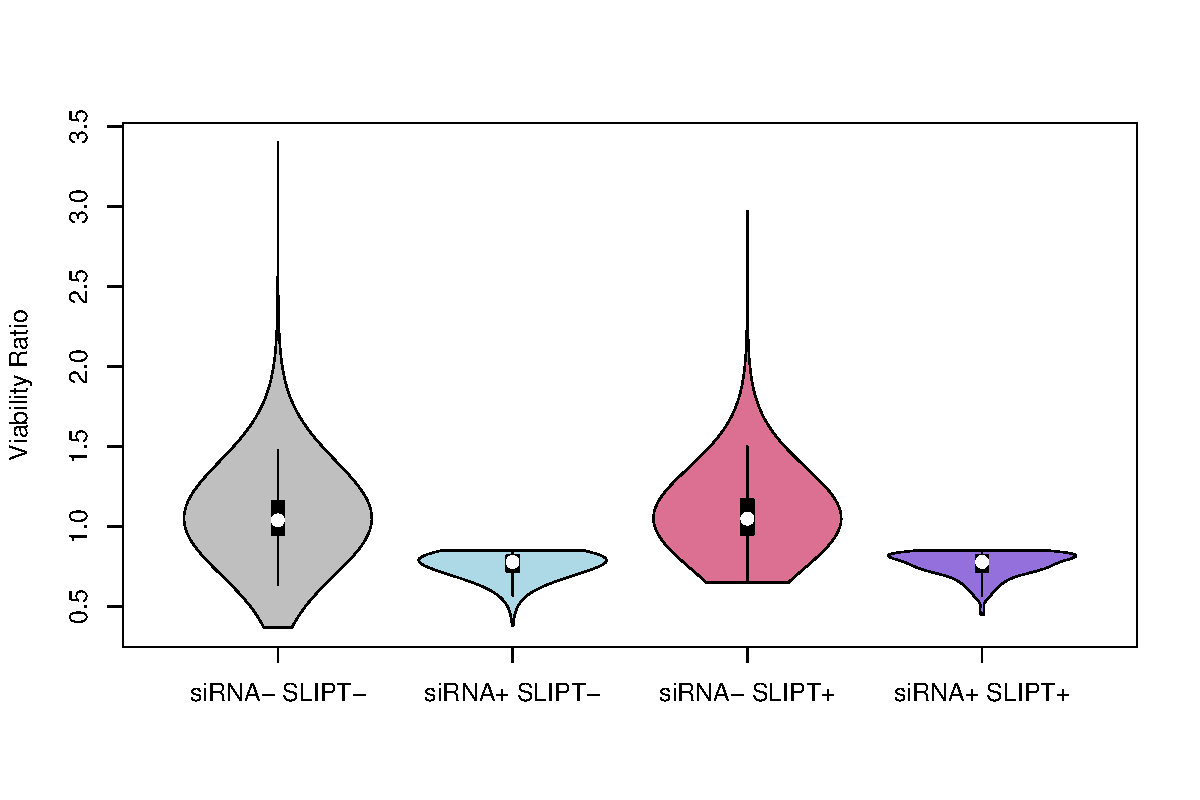
\includegraphics{vioplotx_mtSLIPT_siRNA_vs_Viability_Ratio_with_CDH1.pdf}
   }
   \end{center}
   \caption[Compare \acrshort{mtSLIPT} and \gls{siRNA} genes with \gls{siRNA} viability]{\small \textbf{Compare \acrshort{mtSLIPT} and \gls{siRNA} genes with \gls{siRNA} viability.}  Genes detected as candidate synthetic lethal partners by \acrshort{mtSLIPT} (in \gls{TCGA} breast cancer) expression analysis against \textit{CDH1} mutation and experimental screening (with \gls{siRNA}) were compared against the viability ratio of \textit{CDH1} mutant and wildtype cells in the primary \gls{siRNA} screen. There were clear no differences in viability between genes detected by \acrshort{mtSLIPT} and those not with the differences being primarily due to viability thresholds that were used to detect synthetic lethality by \citet{Telford2015}. 
}
\label{fig:compare_viability_mtSL}
%\end{mdframed}
\end{figure*}


\clearpage
\section{Metagene Analysis} \label{appendix:metagene_mtSL}

Metagene analysis was performed for synthetic lethal pathways against \textit{CDH1} mutation. These were described and compared to expression analysis in Section~\ref{chapt3:metagene_SL}. 

\begin{table*}[!ht]
\caption{Candidate synthetic lethal metagenes against \textit{CDH1} from mtSLIPT}
\label{tab:metagene_mtSL}
\centering
\resizebox{1 \textwidth}{!}{
\begin{threeparttable}
\begin{tabular}{sl^l^c^c^c^c^c}
\rowstyle{\bfseries}
 Pathway & ID & Observed & Expected & $\chi^2$value & p-value & p-value (\gls{FDR}) \\
  \hline
  \rowcolor{black!10}
  Neurotoxicity of clostridium toxins & 168799 & 8 & 36.7 & 79.4 & $5.71 \times 10^{-18}$ & $3.14 \times 10^{-15}$ \\ 
  \rowcolor{black!5}
  Aquaporin-mediated transport & 445717 & 8 & 36.7 & 76.3 & $2.73 \times 10^{-17}$ & $9.01 \times 10^{-15}$ \\ 
  \rowcolor{black!10}
  Toxicity of botulinum toxin type G (BoNT/G) & 5250989 & 8 & 36.7 & 76.3 & $2.73 \times 10^{-17}$ & $9.01 \times 10^{-15}$ \\ 
  \rowcolor{black!5}
  ABC-family proteins mediated transport & 382556 & 10 & 36.7 & 68.2 & $1.58 \times 10^{-15}$ & $1.86 \times 10^{-13}$ \\ 
  \rowcolor{black!10}
 G$_{\alpha z}$ signalling events & 418597 & 10 & 36.7 & 59.9 & $9.97 \times 10^{-14}$ & $5.48 \times 10^{-12}$ \\ 
  \rowcolor{black!5}
  Regulation of IGF transport and uptake by IGFBPs  & 381426 & 9 & 36.7 & 56.3 & $5.88 \times 10^{-13}$ & $2.11 \times 10^{-11}$ \\ 
  \rowcolor{black!10}
  GP1b-IX-V activation signalling & 430116 & 8 & 36.7 & 55.7 & $8.20 \times 10^{-13}$ & $2.76 \times 10^{-11}$ \\ 
  \rowcolor{black!5}
  GABA receptor activation & 977443 & 12 & 36.7 & 55.1 & $1.07 \times 10^{-12}$ & $3.26 \times 10^{-11}$ \\ 
  \rowcolor{black!10}
  Vasopressin regulates renal water homeostasis via Aquaporins & 432040 & 9 & 36.7 & 54.1 & $1.77 \times 10^{-12}$ & $4.88 \times 10^{-11}$ \\ 
  \rowcolor{black!5}
  Toxicity of botulinum toxin type D (BoNT/D) & 5250955 & 14 & 36.7 & 53.4 & $2.54 \times 10^{-12}$ & $6.64 \times 10^{-11}$ \\ 
  \rowcolor{black!10}
  Toxicity of botulinum toxin type F (BoNT/F) & 5250981 & 14 & 36.7 & 53.4 & $2.54 \times 10^{-12}$ & $6.64 \times 10^{-11}$ \\ 
  \rowcolor{black!5}
  STAT6-mediated induction of chemokines & 3249367 & 16 & 36.7 & 52.2 & $4.72 \times 10^{-12}$ & $1.13 \times 10^{-10}$ \\ 
  \rowcolor{black!10}
  Toxicity of botulinum toxin type B (BoNT/B) & 5250958 & 14 & 36.7 & 50.8 & $9.5 \times 10^{-12}$ & $1.98 \times 10^{-10}$ \\ 
  \rowcolor{black!5}
  S6K1 signalling & 165720 & 12 & 36.7 & 50.2 & $1.24 \times 10^{-11}$ & $2.5 \times 10^{-10}$ \\ 
  \rowcolor{black!10}
 G$_{\alpha s}$ signalling events & 418555 & 11 & 36.7 & 49.2 & $2.08 \times 10^{-11}$ & $3.85 \times 10^{-10}$ \\ 
  \rowcolor{black!5}
  RHO GTPases activate CIT & 5625900 & 14 & 36.7 & 48.2 & $3.34 \times 10^{-11}$ & $5.9 \times 10^{-10}$ \\ 
  \rowcolor{black!10}
  NADE modulates death signalling & 205025 & 15 & 36.7 & 47.4 & $5.00 \times 10^{-11}$ & $8.32 \times 10^{-10}$ \\ 
  \rowcolor{black!5}
  Keratan sulfate degradation & 2022857 & 10 & 36.7 & 46.6 & $7.5 \times 10^{-11}$ & $1.15 \times 10^{-9}$ \\ 
  \rowcolor{black!10}
  Signalling by Retinoic Acid & 5362517 & 10 & 36.7 & 46.6 & $7.5 \times 10^{-11}$ & $1.15 \times 10^{-9}$ \\ 
  \rowcolor{black!5}
  Adenylate cyclase inhibitory pathway & 170670 & 14 & 36.7 & 45.9 & $1.11 \times 10^{-10}$ & $1.59 \times 10^{-9}$ \\ 
  \rowcolor{black!10}
  Inhibition of adenylate cyclase pathway & 997269 & 14 & 36.7 & 45.9 & $1.11 \times 10^{-10}$ & $1.59 \times 10^{-9}$ \\ 
  \rowcolor{black!5}
  Fatty acids & 211935 & 6 & 36.7 & 45.7 & $1.21 \times 10^{-10}$ & $1.72 \times 10^{-9}$ \\ 
  \rowcolor{black!10}
  Ionotropic activity of Kainate Receptors & 451306 & 13 & 36.7 & 44.6 & $2.03 \times 10^{-10}$ & $2.58 \times 10^{-9}$ \\ 
  \rowcolor{black!5}
  Activation of Ca-permeable Kainate Receptor & 451308 & 13 & 36.7 & 44.6 & $2.03 \times 10^{-10}$ & $2.58 \times 10^{-9}$ \\ 
  \rowcolor{black!10}
  RA biosynthesis pathway & 5365859 & 13 & 36.7 & 44.6 & $2.03 \times 10^{-10}$ & $2.58 \times 10^{-9}$ \\ 
   \hline
\end{tabular}
\begin{tablenotes}
\raggedright \small
Strongest candidate \gls{synthetic lethal} partners for \textit{CDH1} by \acrshort{mtSLIPT} with observed and expected numbers of mutant \textit{CDH1} \gls{TCGA} breast cancer tumours with low expression of partner metagenes.
\end{tablenotes}
\end{threeparttable}
}
\end{table*}

\iffalse
\clearpage
\section{Mutation Variation} \label{appendix:mutation_analysis}
Mutations have different effects as shown by the following examples in cancer genes.

\subsection{Mutation Frequency}

%Mutation_locus_PIK3CA.pdf
%Mutation_locus_CDH1.pdf
%Mutation_locus_TP53.pdf

\begin{figure*}[!ht]
%\begin{mdframed}
        \begin{center}
%
        \subcaptionbox{\textit{PI3KCA} \label{fig:mutation_locus:PIK3CA}}{%
            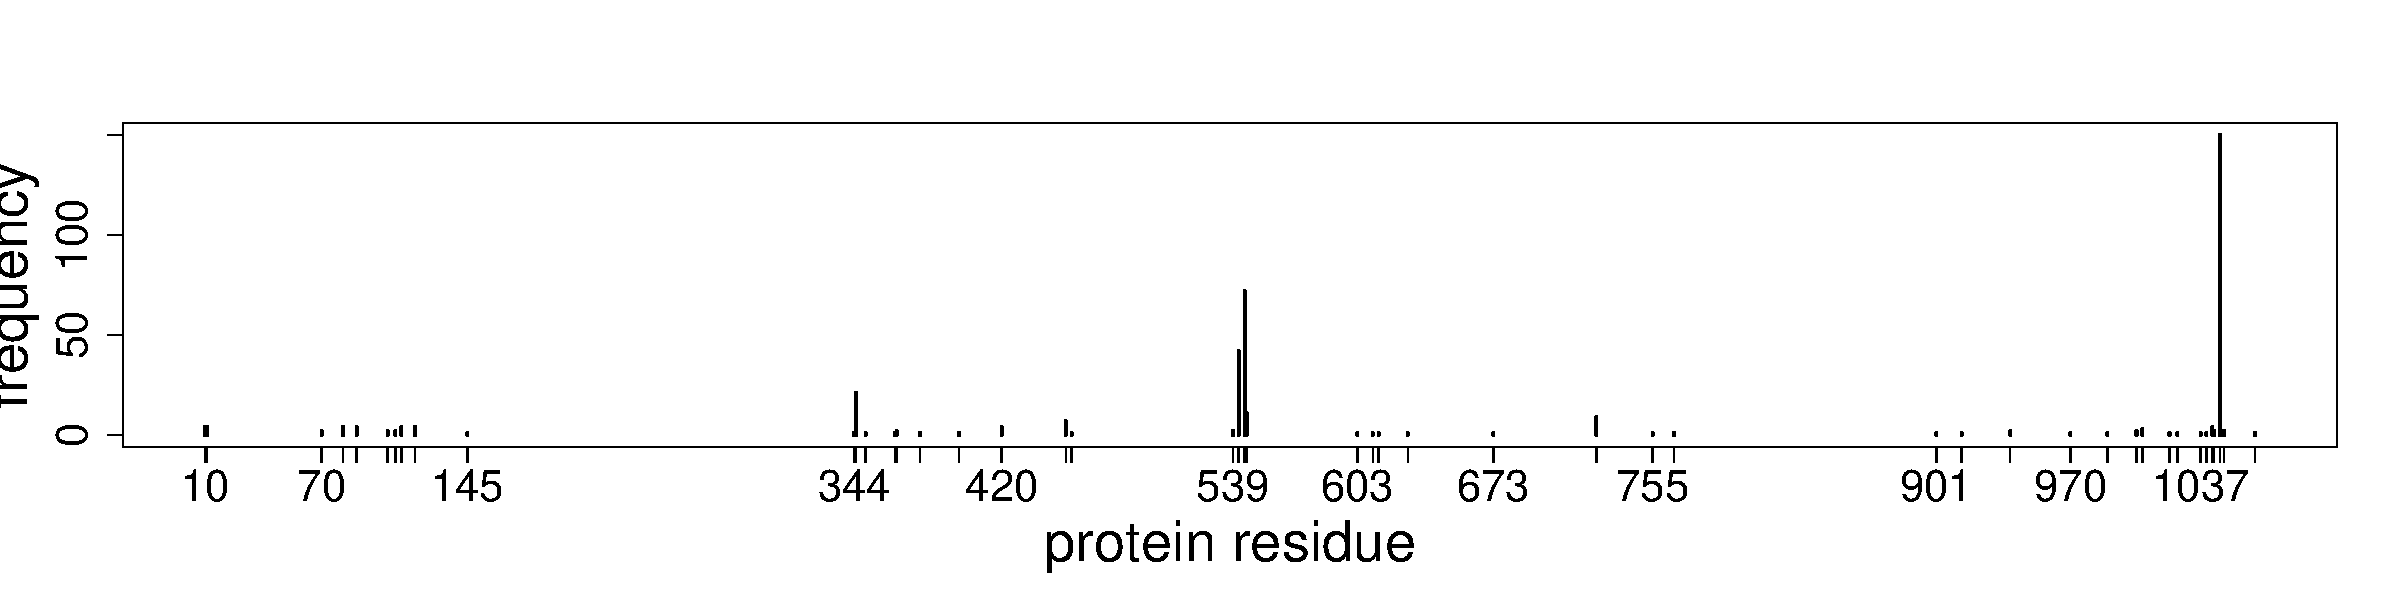
\includegraphics[width=0.75\textwidth]{Mutation_locus_PIK3CA.pdf}
        }
        \subcaptionbox{\textit{PI3KR1} \label{fig:mutation_locus:PIK3R1}}{%
            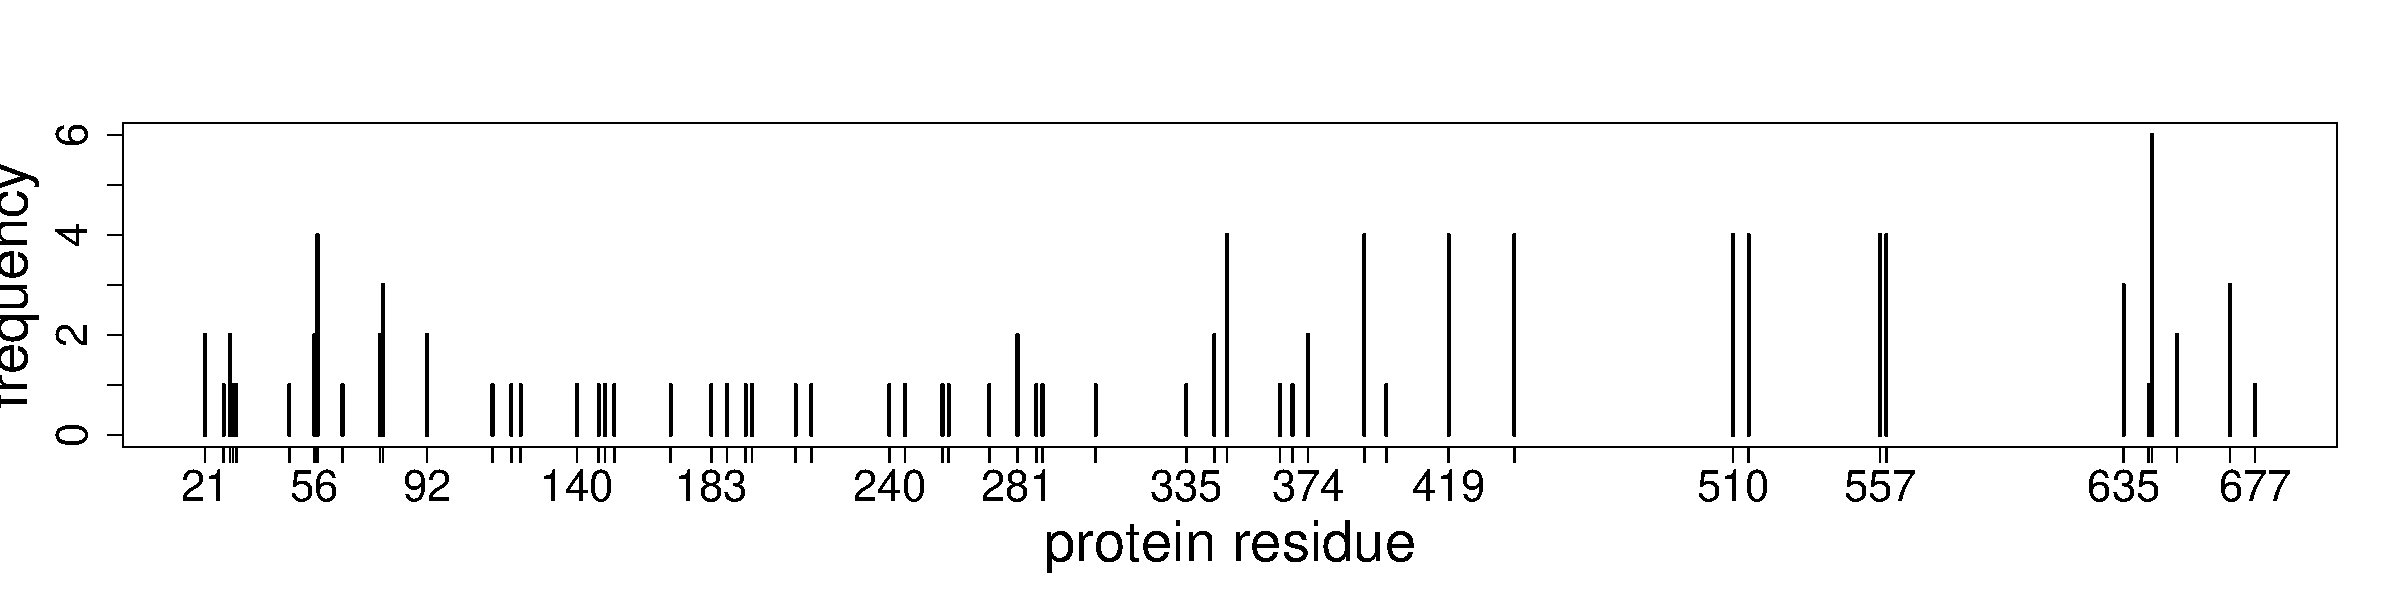
\includegraphics[width=0.75\textwidth]{Mutation_locus_PIK3R1.pdf}
        }
        \subcaptionbox{\textit{CDH1} \label{fig:mutation_locus:CDH1}}{%
           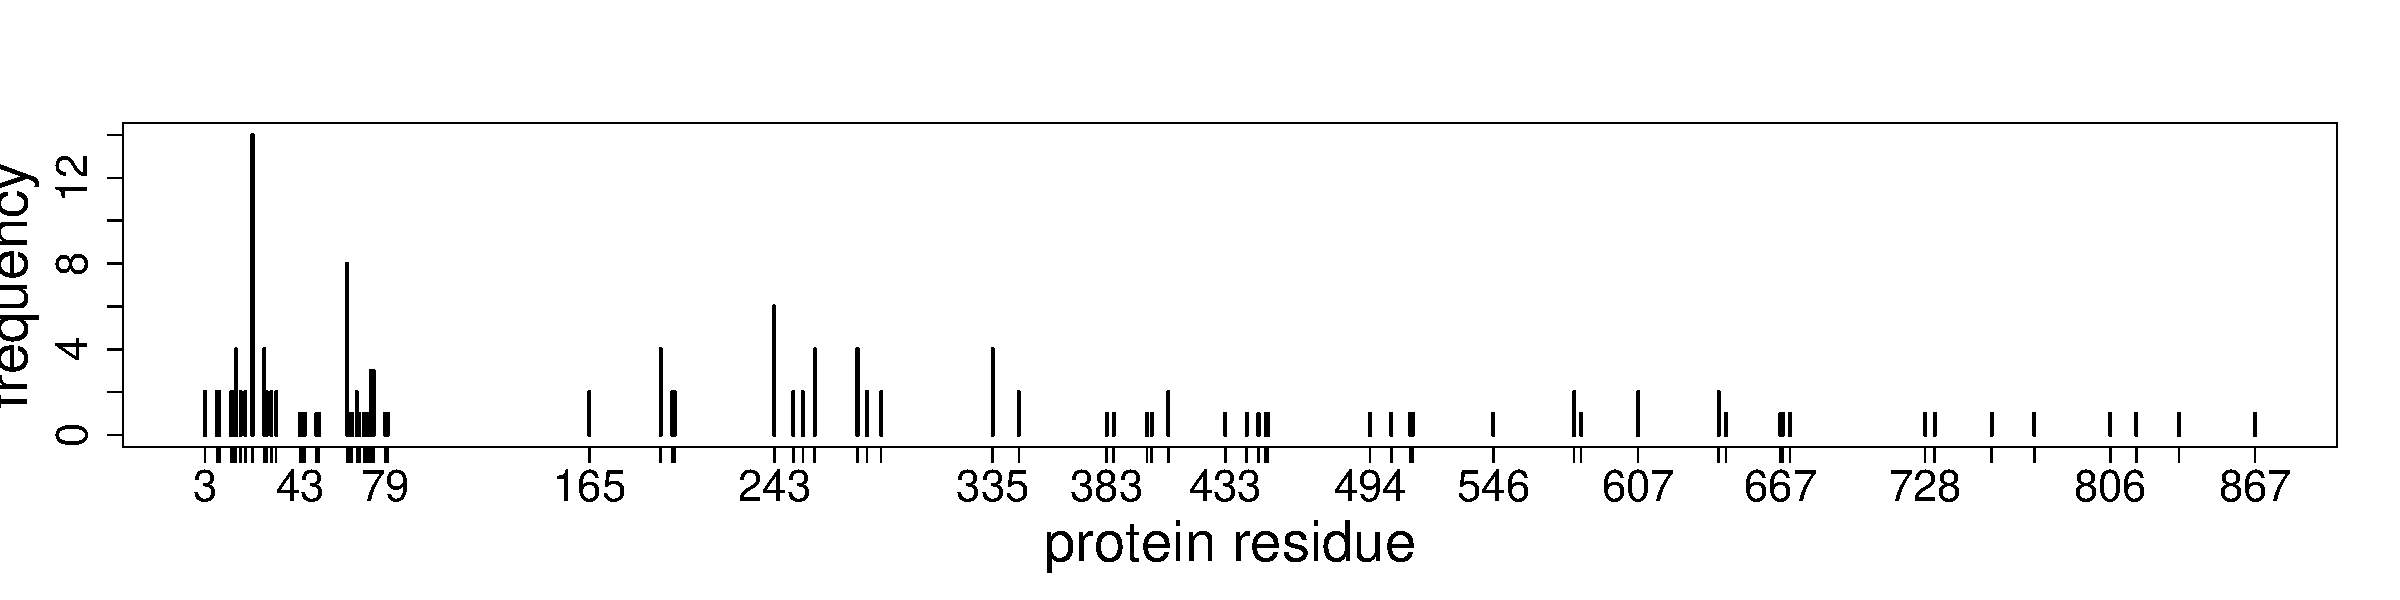
\includegraphics[width=0.75\textwidth]{Mutation_locus_CDH1.pdf}
        }
        \subcaptionbox{\textit{TP53} \label{fig:mutation_locus:TP53}}{%
           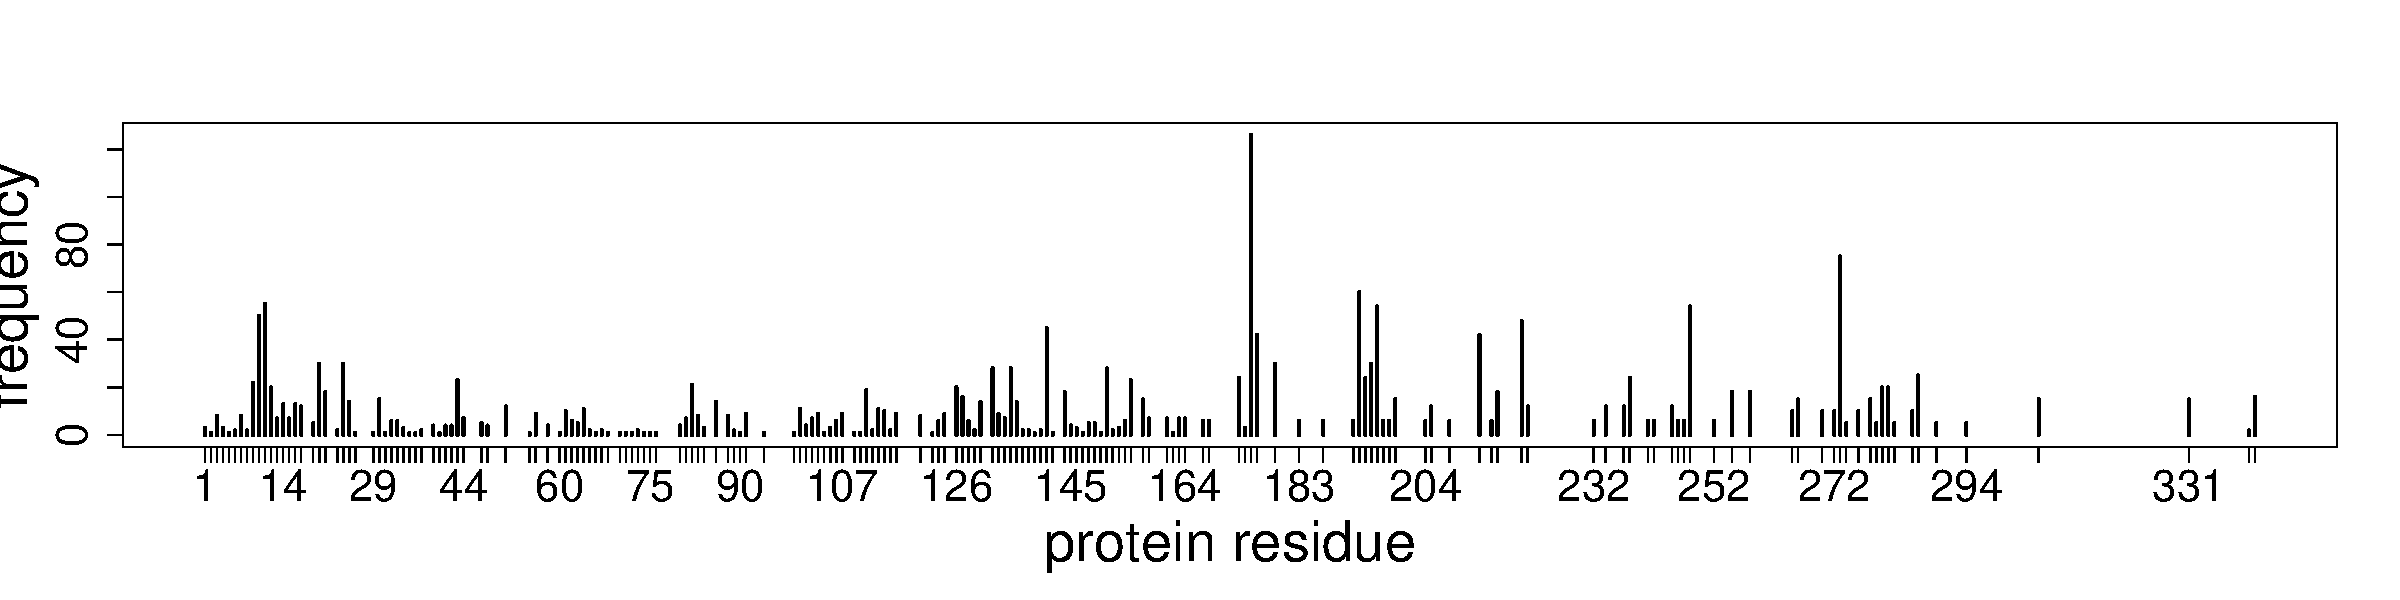
\includegraphics[width=0.75\textwidth]{Mutation_locus_TP53.pdf}
        }
    \end{center}
    \caption[Somatic mutation locus]{\small \textbf{Somatic mutation locus.} Mutation frequency at each locus in \gls{TCGA} breast cancer. \textit{PIK3CA} shows clear recurrent E545K and H1047R oncogene mutations consistent with it being an oncogene. \textit{PIK3R1} and \textit{CDH1} were tumour suppressors with inactivating mutations distributed throughout the gene, whereas \textit{TP53} exhibits both of these properties and a very high mutation frequency compared to other genes.
}
\label{fig:mutation_locus}
%\end{mdframed}
\end{figure*}
\fi

\clearpage
\section{Expression of Somatic Mutations}

\begin{figure*}[!ht]
%\begin{mdframed}
        \begin{center}
%
        \subcaptionbox{\textit{PIK3CA} mutation}{%
           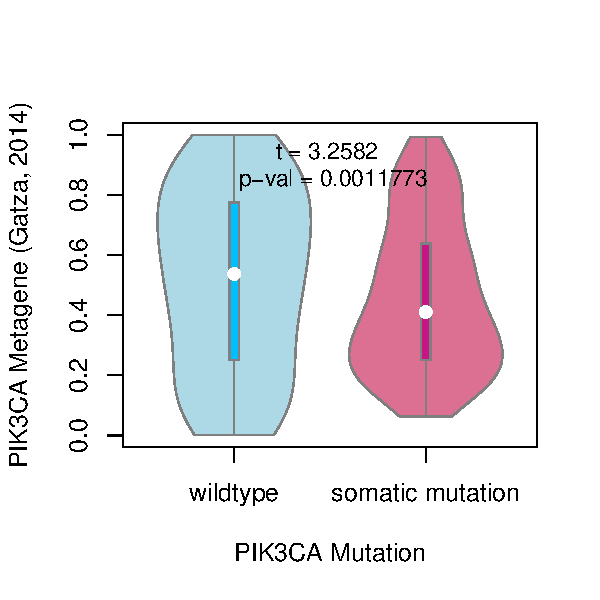
\includegraphics[width=0.45\textwidth]{metagene(ranked)_vioplotx_Mutation_PIK3CA2014_PIK3CA.pdf}
        }%
        \subcaptionbox{\textit{PIK3CA} or \textit{PIK3R1} mutation}{%
           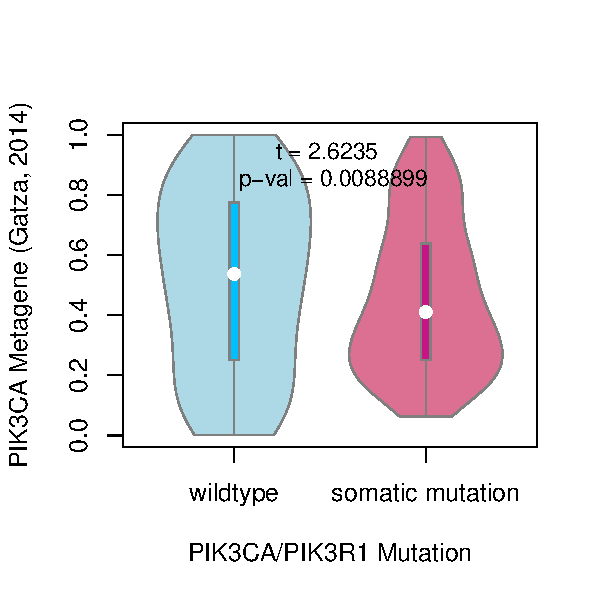
\includegraphics[width=0.45\textwidth]{metagene(ranked)_vioplotx_Mutation_PIK3CA2014_PIK3CA_PIK3R1.pdf}
        }
        
        \subcaptionbox{\textit{CDH1} mutation}{%
           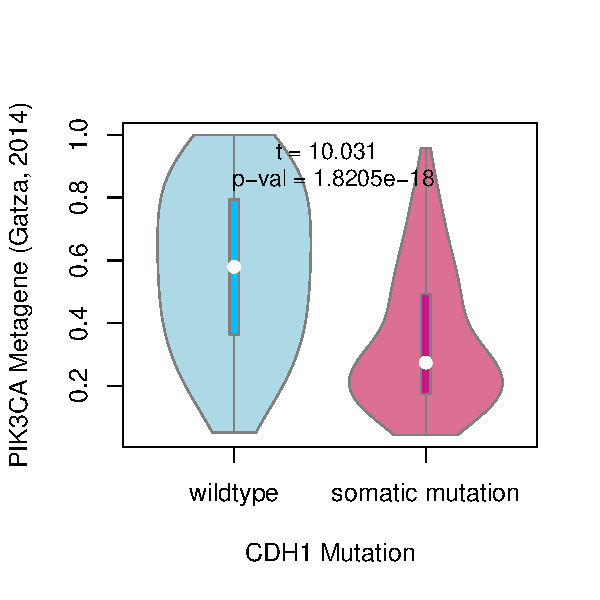
\includegraphics[width=0.45\textwidth]{metagene(ranked)_vioplotx_Mutation_PIK3CA2014_CDH1.pdf}
        }%
        \subcaptionbox{\textit{TP53} mutation}{%
           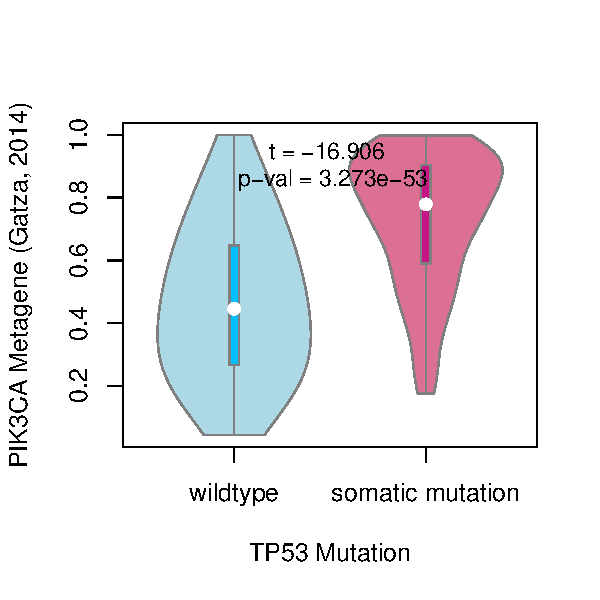
\includegraphics[width=0.45\textwidth]{metagene(ranked)_vioplotx_Mutation_PIK3CA2014_TP53.pdf}
        }
    \end{center}
    \caption[Somatic mutation against PIK3CA metagene]{\small \textbf{Somatic mutation against PIK3CA metagene.} Mutations in \textit{PIK3CA}, \textit{PIK3R1}, \textit{CDH1}, and \textit{TP53} were examined in \gls{TCGA} breast cancer for their effect on the PIK3CA  \citep{Gatza2014} pathway metagene. The tumour suppressors \textit{CDH1} and \textit{TP53} showed an increase and decrease in the metagene respectively, whereas \textit{PIK3CA} and \textit{PIK3R1} mutations weaker evidence of decrease in metagene levels.
}
\label{fig:mutation_expr_mg2}
%\end{mdframed}
\end{figure*}
\fi


%\iffalse
\begin{figure*}[!ht]
%\begin{mdframed}
        \begin{center}
%
        \subcaptionbox{\textit{PIK3CA} mutation}{%
           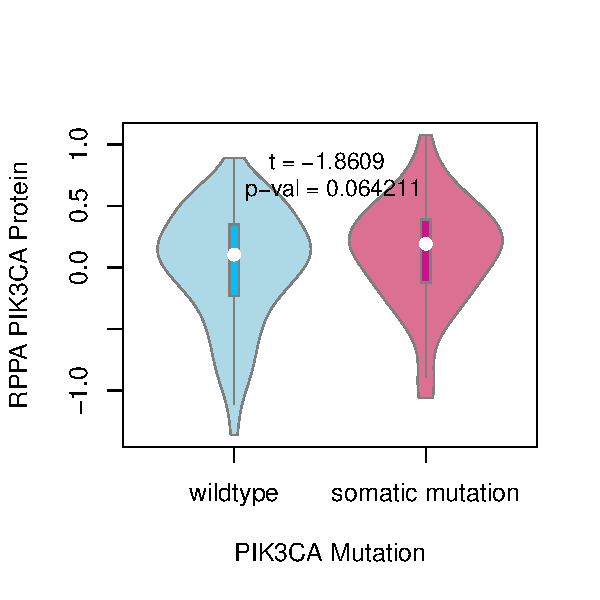
\includegraphics[width=0.45\textwidth]{protein_vioplotx_Mutation_PI3K_PIK3CA.pdf}
        }%
        \subcaptionbox{\textit{PIK3CA} or \textit{PIK3R1} mutation}{%
           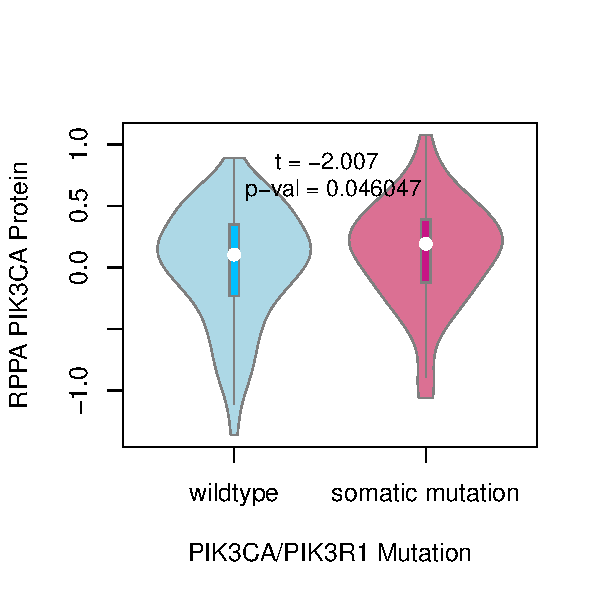
\includegraphics[width=0.45\textwidth]{protein_vioplotx_Mutation_PI3K_PIK3CA_PIK3R1.pdf}
        }
        
        \subcaptionbox{\textit{CDH1} mutation}{%
           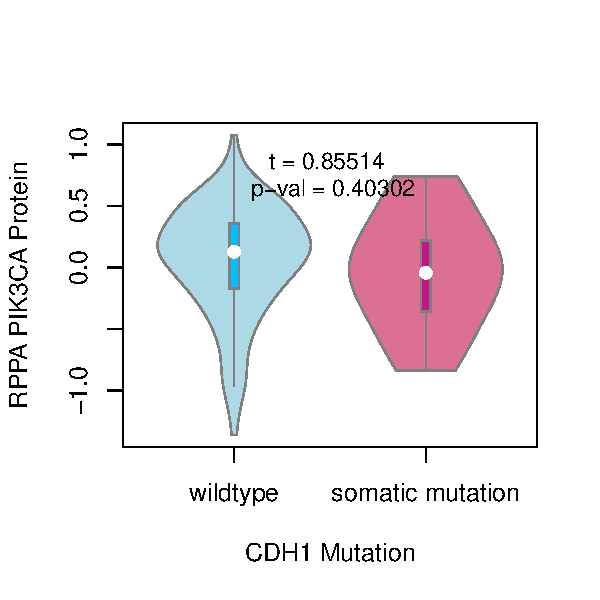
\includegraphics[width=0.45\textwidth]{protein_vioplotx_Mutation_PI3K_CDH1.pdf}
        }%
        \subcaptionbox{\textit{TP53} mutation}{%
           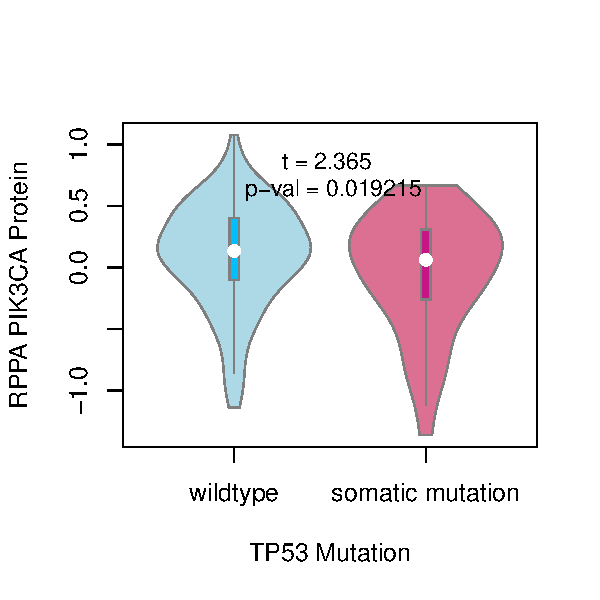
\includegraphics[width=0.45\textwidth]{protein_vioplotx_Mutation_PI3K_TP53.pdf}
        }
    \end{center}
    \caption[Somatic mutation against PI3K protein]{\small \textbf{Somatic mutation against PI3K protein.} Mutations in \textit{PIK3CA}, \textit{PIK3R1}, \textit{CDH1}, and \textit{TP53} were examined in \gls{TCGA} breast cancer for their effect on the expression of the p110$\alpha$ protein (encoded by \textit{PIK3CA}). Protein levels were significantly elevated in samples with \textit{PIK3CA} or \textit{PIK3R1} mutations and lower in samples with \textit{TP53} mutations.
}
\label{fig:mutation_expr_prot}
%\end{mdframed}
\end{figure*}

\begin{figure*}[!ht]
%\begin{mdframed}
        \begin{center}
%
        \subcaptionbox{\textit{PIK3CA} mutation}{%
           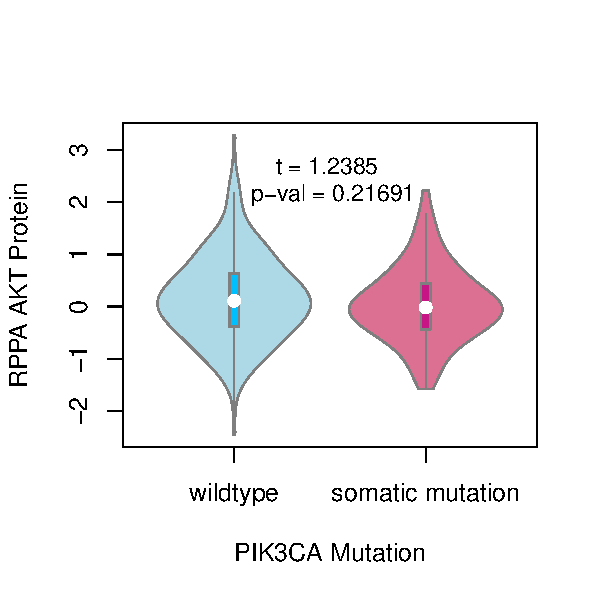
\includegraphics[width=0.45\textwidth]{protein_vioplotx_Mutation_AKT_PIK3CA.pdf}
        }%
        \subcaptionbox{\textit{PIK3CA} or \textit{PIK3R1} mutation}{%
           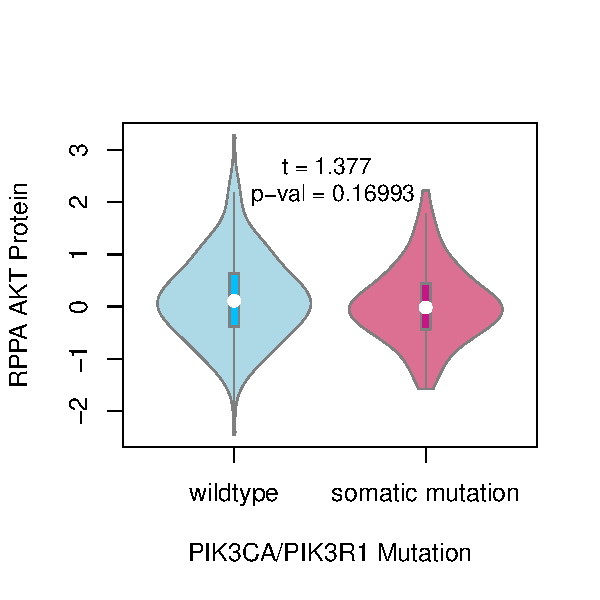
\includegraphics[width=0.45\textwidth]{protein_vioplotx_Mutation_AKT_PIK3CA_PIK3R1.pdf}
        }
        
        \subcaptionbox{\textit{CDH1} mutation}{%
           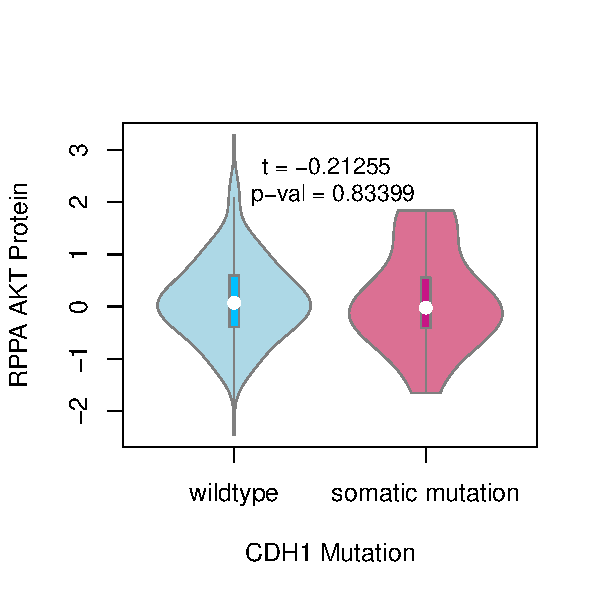
\includegraphics[width=0.45\textwidth]{protein_vioplotx_Mutation_AKT_CDH1.pdf}
        }%
        \subcaptionbox{\textit{TP53} mutation}{%
           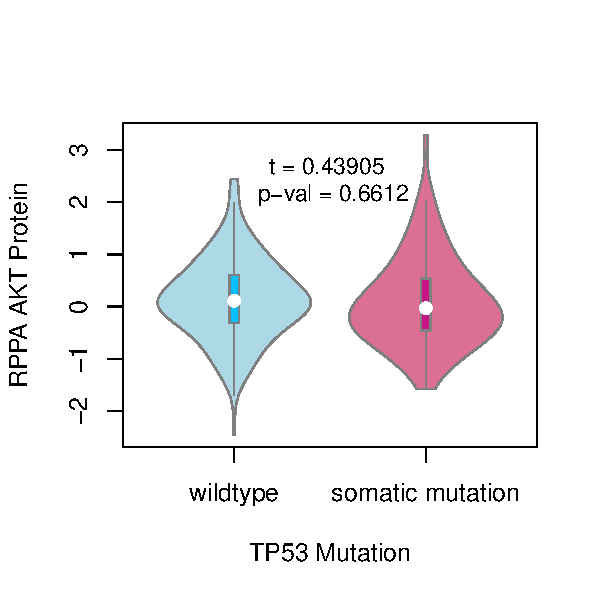
\includegraphics[width=0.45\textwidth]{protein_vioplotx_Mutation_AKT_TP53.pdf}
        }
    \end{center}
    \caption[Somatic mutation against AKT protein]{\small \textbf{Somatic mutation against AKT protein.} Mutations in \textit{PIK3CA}, \textit{PIK3R1}, \textit{CDH1}, and \textit{TP53} were examined in \gls{TCGA} breast cancer for their effect on the expression of the AKT protein (a downstream target of \textit{PIK3CA}). Protein levels were not significantly different in samples mutations in any of these cancer genes.
}
\label{fig:mutation_expr_prot2}
%\end{mdframed}
\end{figure*}
%\fi

\clearpage
\section{Metagene Expression Profiles}
\label{appendix:mg_expr_SL}

%\label{fig:metagene_expr_Gatza2011}


\begin{figure*}[!htp]
\noindent\makebox[\textwidth][c]{%               %centering
%\noindent\fbox{
\begin{minipage}{1.15 \textwidth}  %frame beyond textwidth
\begin{center}
  \resizebox{1 \textwidth}{!}{
    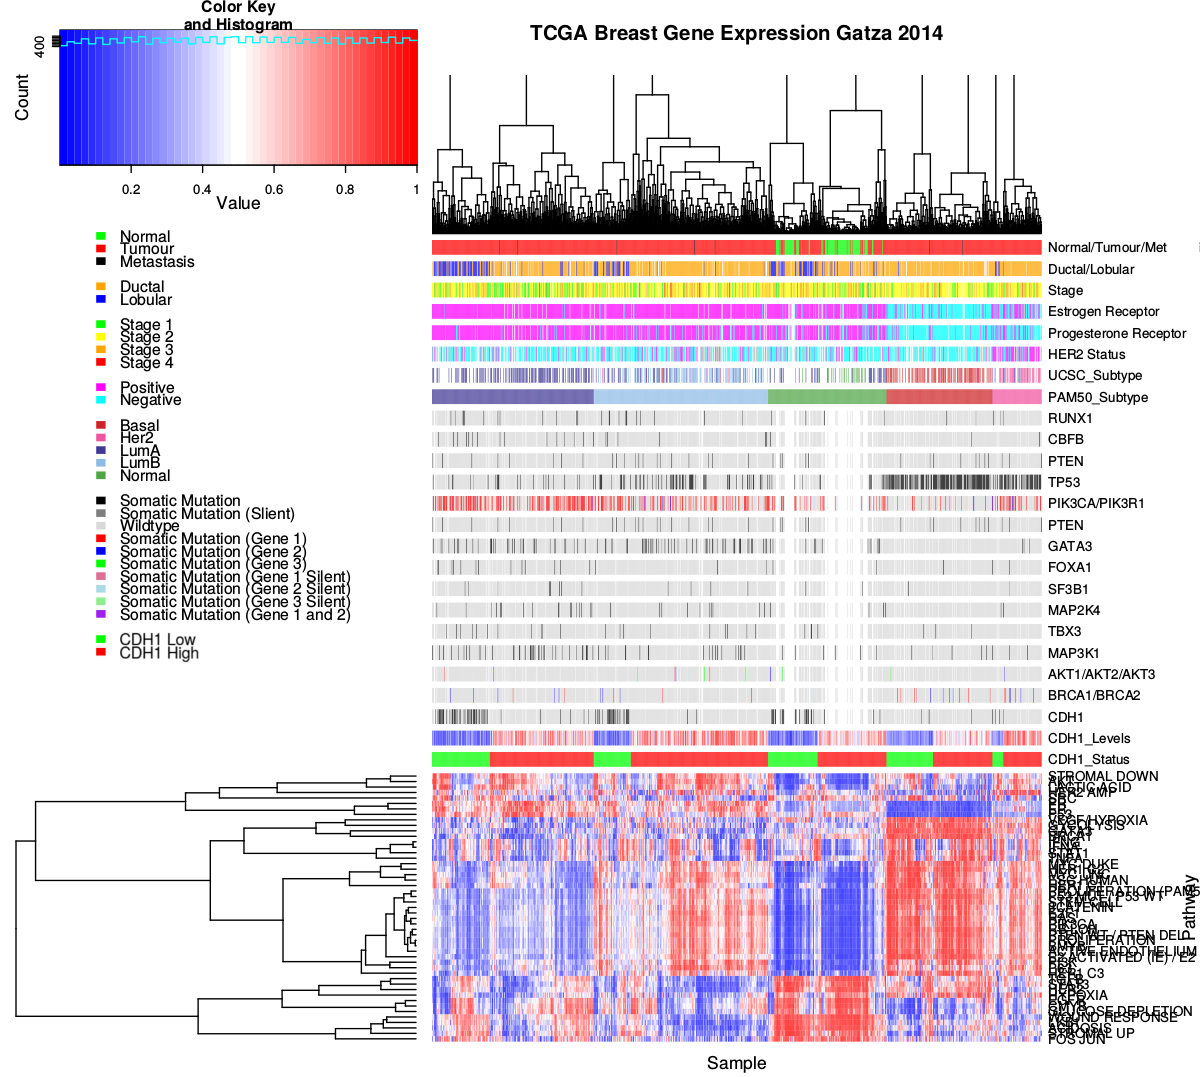
\includegraphics{CDH1_Heatmaps_Gatza2014(ranked)_Full_split_by_Subtype_and_CDH1_Stat_corr.png} %original pdf, png for edited
   }
   \end{center}
   \caption[Pathway metagene expression profiles]{\small \textbf{Pathway metagene expression profiles.} Expression profiles for metagene signatures from \citet{Gatza2014} in \gls{TCGA} breast data, annotated for clinical factors and cancer gene mutations.
}
\label{fig:metagene_expr_Gatza2014}
\end{minipage}
%} %close fbox
} %close centering
\end{figure*}

\begin{figure*}[!htp]
\noindent\makebox[\textwidth][c]{%               %centering
%\noindent\fbox{
\begin{minipage}{1.15 \textwidth}  %frame beyond textwidth
\begin{center}
  \resizebox{1 \textwidth}{!}{
    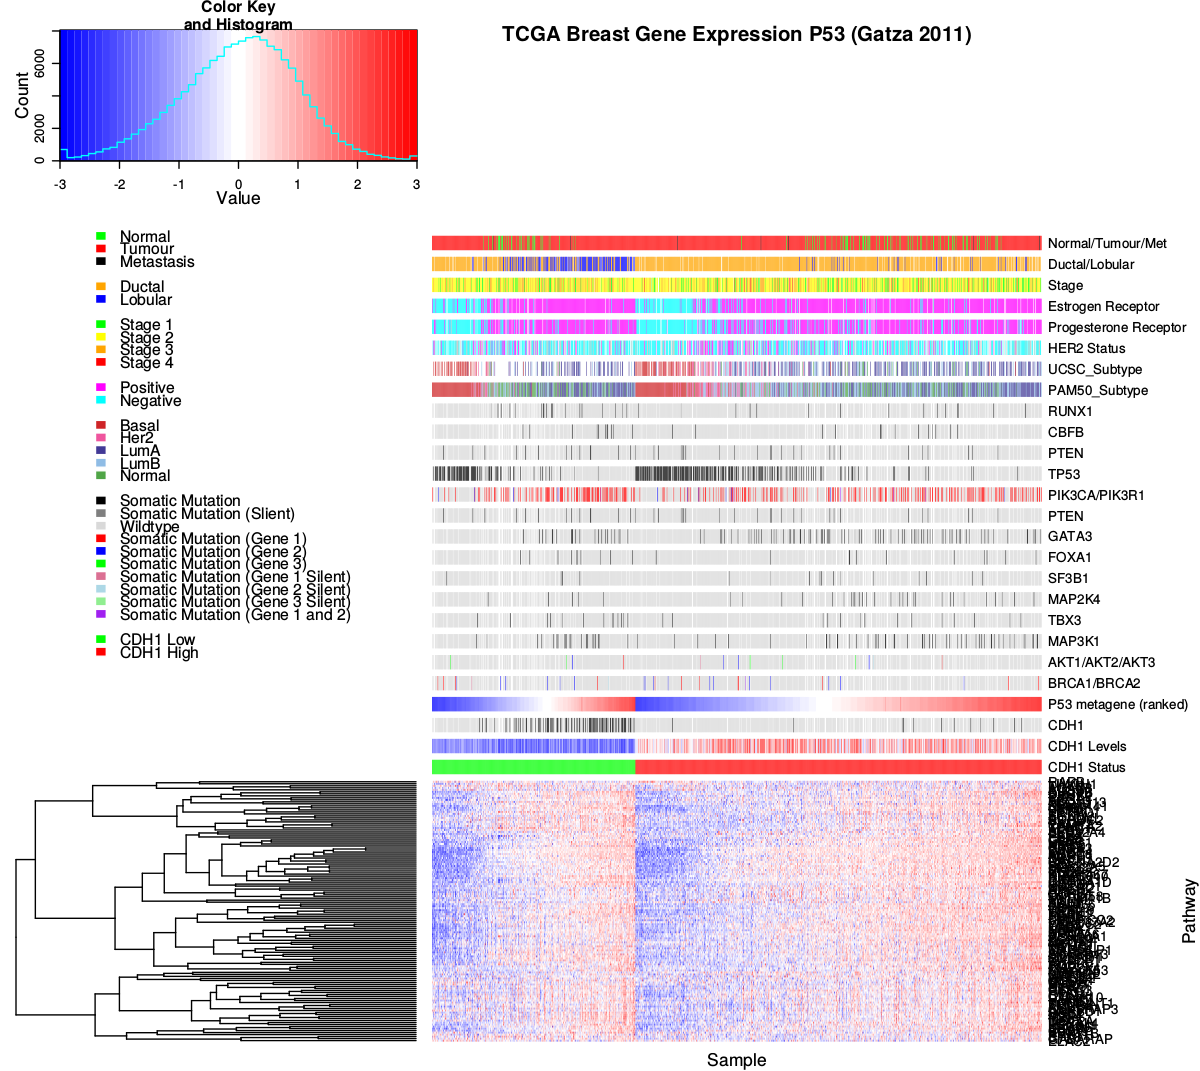
\includegraphics{CDH1_Heatmaps_Gatza2011(P53)_Full_Metagene_mgorder.png} %original pdf, png for edited
   }
   \end{center}
   \caption[Expression profiles for p53 related genes]{\small \textbf{Expression profiles for p53 related genes.} Expression profiles the genes contained in the \textit{TP53} gene signature from \citet{Gatza2011} in \gls{TCGA} breast data, annotated for clinical factors and cancer gene mutations. Samples were separated by \textit{CDH1} expression status and sorted by the metagene. In both cases, the majority of genes were consistent with the direction of the metagene, with few very exceptions. \textit{TP53} mutant samples had low metagene expression, consistent with loss of tumour suppressor functions, and were less likely to have \textit{CDH1} or \textit{PIK3CA} mutations.
}
\label{fig:metagene_expr_Gatza2011_P53}
\end{minipage}
%} %close fbox
} %close centering
\end{figure*}

\begin{figure*}[!htp]
\noindent\makebox[\textwidth][c]{%               %centering
%\noindent\fbox{
\begin{minipage}{1.15 \textwidth}  %frame beyond textwidth
\begin{center}
  \resizebox{1 \textwidth}{!}{
    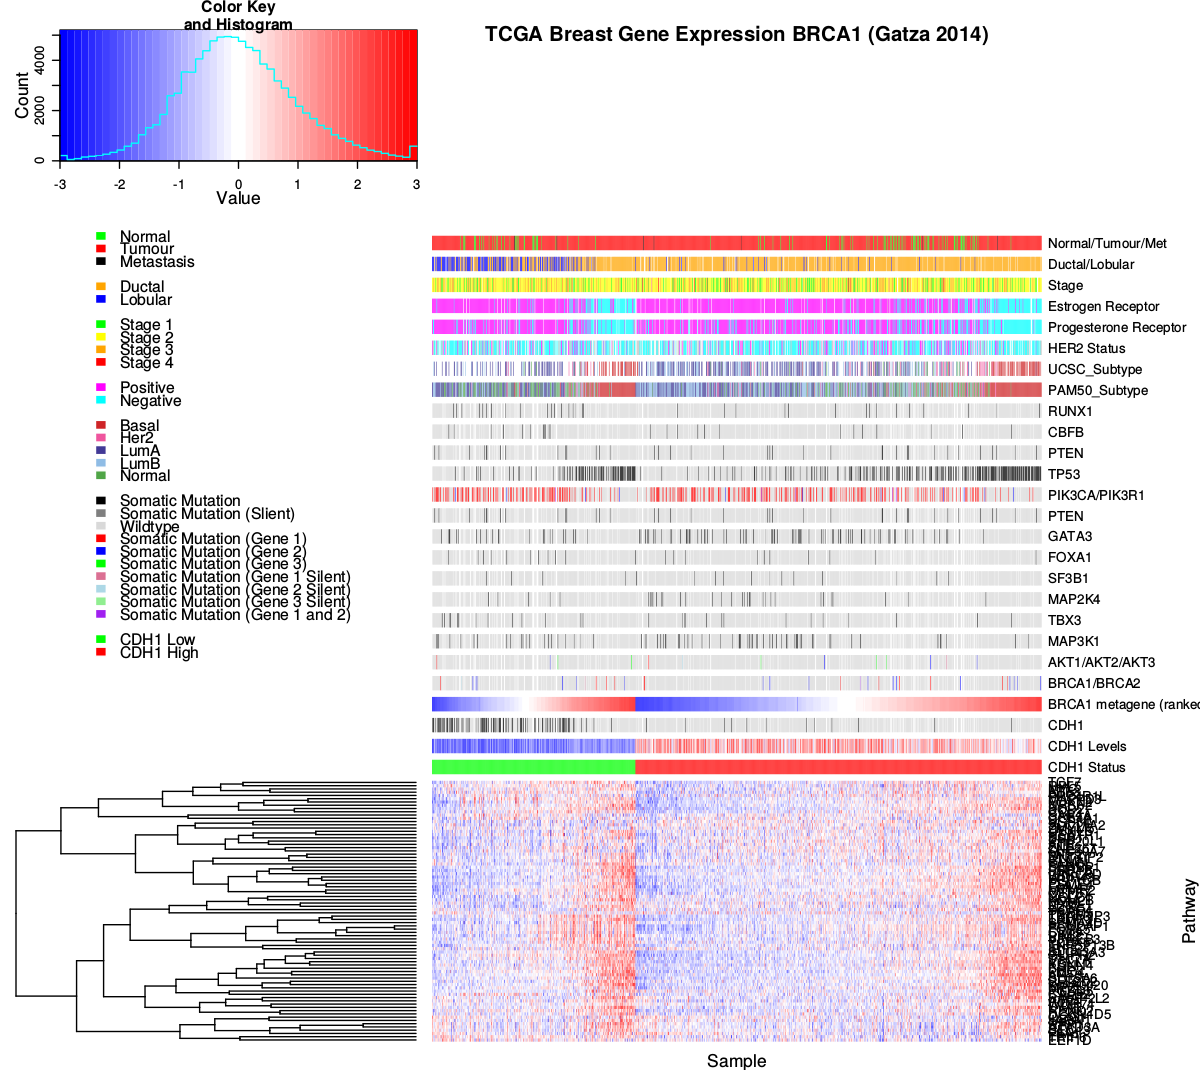
\includegraphics{CDH1_Heatmaps_Gatza2014(BRCA1)_Full_Metagene_mgorder.png} %original pdf, png for edited
   }
   \end{center}
   \caption[Expression profiles for BRCA related genes]{\small \textbf{Expression profiles for BRCA related genes.} Expression profiles the genes contained in the gene signature related to \textit{BRCA1} and \textit{BRCA2} functions from \citet{Gatza2014} in \gls{TCGA} breast data, annotated for clinical factors and cancer gene mutations. Samples were separated by \textit{CDH1} expression status and sorted by the metagene. In both cases, the majority of genes were consistent with the direction of the metagene, with few very exceptions. \textit{BRCA1} and \textit{BRCA2} mutant samples had higher metagene expression than most samples for the ductal subtype, although this was not the case (for the lobular samples for which the metagene was lower). However, the metagene was higher for basal subtype and \acrshort{ER} negative samples.
}
\label{fig:metagene_expr_Gatza2014_BRCA}
\end{minipage}
%} %close fbox
} %close centering
\end{figure*}

\FloatBarrier


\clearpage
\chapter{Intrinsic Subtyping} \label{appendix:intrinsic_subtypes}
The intrinsic subtypes for \gls{TCGA} breast cancer samples provided by \gls{UCSC} \citep{TCGA2012, UCSC2012} that were derived from microarray analysis have been compared to the \gls{PAM50} results for performing subtyping from \gls{RNA-Seq} data \citep{Parker2009}. As shown in Table~\ref{tab:intrinsic_subtypes}, these subtypes were highly concordant for samples which had both procedures performed upon them ($\chi^2 = 1305.9$, $p = 2.73 \times 10^{-268}$). The main exception were the luminal A samples some of which were reclassified as luminal B or ``normal-like''.

\begin{table*}[!htb]
\caption{Comparison of intrinsic subtypes}
\label{tab:intrinsic_subtypes}
\noindent\makebox[\textwidth][c]{%               %centering
\resizebox{0.8 \textwidth}{!}{
\begin{threeparttable}
\begin{tabular}{llllll}
 \cellcolor{white} & \multicolumn{5}{c}{\bfseries \gls{UCSC} Subtype}  \\  
\cline{2-6}
 \cellcolor{white} & Basal-like &  HER2-enriched  &  Luminal A  &  Luminal B  &  Normal-like  \\
\cline{2-6}
\rowcolor{black!10} \cellcolor{white}
 \cellcolor{white} &    100  &   58  &  232  &  128  &  30  \\
\cline{2-6}
%\end{tabular}
\\
%\begin{tabular}{llllll}
 \cellcolor{white} & \multicolumn{5}{c}{\bfseries \gls{PAM50} Subtype}  \\
\cline{2-6}
 \cellcolor{white} & Basal-like &  HER2-enriched  &  Luminal A  &  Luminal B  &  Normal-like  \\
\cline{2-6}
\rowcolor{black!10} \cellcolor{white}
 \cellcolor{white} &    208  &   94  &  314  &  334  &  227  \\
\cline{2-6}
%\end{tabular}
\\
%\begin{tabular}{lllllll}
 \cellcolor{white} & \multicolumn{5}{c}{\bfseries \gls{UCSC} Subtype}  \\
   \cline{2-6}
 \textbf{\gls{PAM50} Subtype} & Basal-like &  HER2-enriched  &  Luminal A  &  Luminal B  &  Normal-like  \\
   \hline
\rowcolor{black!10} Basal-like    &  96 &   4 &   2 &   2 &   1 \\ 
\rowcolor{black!5} HER2-enriched &   0 &  47 &   5 &   3 &   0 \\ 
\rowcolor{black!10} Luminal A     &   1 &   0 & 141 &   1 &   0 \\ 
\rowcolor{black!5} Luminal B     &   2 &   7 &  49 & 121 &   0 \\ 
\rowcolor{black!10} Normal-like   &   1 &   0 &  35 &   1 &  29 \\ 
  \hline
\end{tabular}
\begin{tablenotes}
\raggedright \small
The intrinsic subtypes of \gls{TCGA} breast samples were compared between those provided by \gls{UCSC} \citep{TCGA2012} from microarray expression to those derived from \gls{RNA-Seq} data \citep{Parker2009}. Comparisons between these were limited to samples for which both data types were available.
\end{tablenotes}
\end{threeparttable}
}
}
\end{table*} 

The \gls{PAM50} subtypes could be more accurate given similarity of these subtypes and that the remainder of the subtypes were accurately recapitulated with \gls{RNA-Seq} data. Furthermore, \gls{UCSC} subtypes correctly identified $\sfrac{22}{22}$ normal samples as ``normal-like'' and \gls{PAM50} subtyping in \gls{RNA-Seq} data had a success rate of $\sfrac{112}{113}$ (including all of those identified from microarrays). Therefore the \gls{PAM50} subtypes (performed on a larger cohort of samples) are appropriate to use for further interpretation, superseding the \gls{UCSC} subtypes available for a limited set of samples.


\FloatBarrier

\chapter{Stomach Expression Analysis}
\label{appendix:stad_exprSL}

The following results are a replication of the \gls{TCGA} results (in Chapter~\ref{chap:SLIPT}) with stomach cancer data, using synthetic lethality (SLIPT) against \textit{CDH1}.

\section{Synthetic Lethal Genes and Pathways} \label{appendix:stad_exprSL_genes}

\begin{table*}[!ht]
\caption{Synthetic lethal gene partners of \textit{CDH1} from SLIPT in stomach cancer}
\label{tab:gene_stad_SL}
\centering
\resizebox{0.6 \textwidth}{!}{
\begin{threeparttable}
\begin{tabular}{>{\em}sl^c^c^c^c^c}
\rowstyle{\bfseries}
 \em{Gene} & Observed\tnote{*}  & Expected\tnote{*} & $\chi^2$ value & p-value & p-value (\gls{FDR}) \\ 
  \hline
  \rowcolor{black!10}
  PRAF2 & 17 & 50.4 & 121 & $3.54 \times 10^{-25}$ & $1.45 \times 10^{-21}$ \\ 
  \rowcolor{black!5}
  EMP3 & 17 & 50.4 & 115 & $5.06 \times 10^{-24}$ & $1.48 \times 10^{-20}$ \\ 
  \rowcolor{black!10}
  PLEKHO1 & 22 & 50.4 & 112 & $2.14 \times 10^{-23}$ & $4.75 \times 10^{-20}$ \\ 
  \rowcolor{black!5}
  SELM & 20 & 50.4 & 111 & $5.13 \times 10^{-23}$ & $8.09 \times 10^{-20}$ \\ 
  \rowcolor{black!10}
  GYPC & 20 & 50.4 & 110 & $5.77 \times 10^{-23}$ & $8.45 \times 10^{-20}$ \\ 
  \rowcolor{black!5}
  COX7A1 & 18 & 50.4 & 109 & $1.15 \times 10^{-22}$ & $1.39 \times 10^{-19}$ \\ 
  \rowcolor{black!10}
  TNFSF12 & 20 & 50.4 & 106 & $4.06 \times 10^{-22}$ & $4.38 \times 10^{-19}$ \\ 
  \rowcolor{black!5}
  SEPT4 & 17 & 50.4 & 106 & $6.58 \times 10^{-22}$ & $5.91 \times 10^{-19}$ \\ 
  \rowcolor{black!10}
  LGALS1 & 19 & 50.4 & 105 & $6.64 \times 10^{-22}$ & $5.91 \times 10^{-19}$ \\ 
  \rowcolor{black!5}
  RARRES2 & 27 & 50.4 & 105 & $8.02 \times 10^{-22}$ & $6.85 \times 10^{-19}$ \\ 
  \rowcolor{black!10}
  VEGFB & 16 & 50.4 & 104 & $1.19 \times 10^{-21}$ & $9.74 \times 10^{-19}$ \\ 
  \rowcolor{black!5}
  PRR24 & 22 & 50.4 & 102 & $2.96 \times 10^{-21}$ & $2.02 \times 10^{-18}$ \\ 
  \rowcolor{black!10}
  SYNC & 19 & 50.4 & 102 & $3.73 \times 10^{-21}$ & $2.39 \times 10^{-18}$ \\ 
  \rowcolor{black!5}
  MAGEH1 & 17 & 50.4 & 100 & $9.52 \times 10^{-21}$ & $5.01 \times 10^{-18}$ \\ 
  \rowcolor{black!10}
  HSPB2 & 23 & 50.4 & 99.6 & $1.19 \times 10^{-20}$ & $5.82 \times 10^{-18}$ \\ 
  \rowcolor{black!5}
  SMARCD3 & 19 & 50.4 & 99 & $1.59 \times 10^{-20}$ & $7.57 \times 10^{-18}$ \\ 
  \rowcolor{black!10}
  CREM & 13 & 50.4 & 98.1 & $2.48 \times 10^{-20}$ & $1.13 \times 10^{-17}$ \\ 
  \rowcolor{black!5}
  GNG11 & 20 & 50.4 & 97.3 & $3.68 \times 10^{-20}$ & $1.59 \times 10^{-17}$ \\ 
  \rowcolor{black!10}
  GNAI2 & 17 & 50.4 & 96.4 & $5.75 \times 10^{-20}$ & $2.36 \times 10^{-17}$ \\ 
  \rowcolor{black!5}
  FUNDC2 & 22 & 50.4 & 95.9 & $7.39 \times 10^{-20}$ & $2.91 \times 10^{-17}$ \\ 
  \rowcolor{black!10}
  CNRIP1 & 21 & 50.4 & 95.3 & $1.0 \times 10^{-19}$ & $3.66 \times 10^{-17}$ \\ 
  \rowcolor{black!5}
  CALHM2 & 22 & 50.4 & 93.1 & $2.94 \times 10^{-19}$ & $1.06 \times 10^{-16}$ \\ 
  \rowcolor{black!10}
  ARID5A & 18 & 50.4 & 92.7 & $3.47 \times 10^{-19}$ & $1.22 \times 10^{-16}$ \\ 
  \rowcolor{black!5}
  ST3GAL3 & 27 & 50.4 & 92.2 & $4.49 \times 10^{-19}$ & $1.56 \times 10^{-16}$ \\ 
  \rowcolor{black!10}
  LOC339524 & 21 & 50.4 & 92.1 & $4.8 \times 10^{-19}$ & $1.59 \times 10^{-16}$ \\ 
  \hline
\end{tabular}
\begin{tablenotes}
\raggedright \small
Strongest candidate \gls{synthetic lethal} partners for \textit{CDH1} by \gls{SLIPT} in \gls{TCGA} stomach cancer expression data

\item[*] Observed and expected numbers of samples which had low \glslink{gene expression}{expression} of both genes
\end{tablenotes}
\end{threeparttable}
}
\end{table*}


\begin{table*}[!ht]
\caption{Pathways for \textit{CDH1} partners from SLIPT in stomach cancer}
\label{tab:pathway_stad_exprSL}
\centering
\resizebox{1 \textwidth}{!}{
\begin{threeparttable}
\begin{tabular}{lccc}
  \cellcolor{white} \textbf{Pathways Over-represented} & \textbf{Pathway Size} & \textbf{SL Genes} & \textbf{p-value (\gls{FDR})} \\
  \hline
  \rowcolor{black!10}
  Extracellular matrix organization & 241 & 104 & $7.5 \times 10^{-140}$ \\ 
  \rowcolor{black!5}
  Hemostasis & 445 & 138 & $1.8 \times 10^{-121}$ \\ 
  \rowcolor{black!10}
  Developmental Biology & 432 & 125 & $9.2 \times 10^{-107}$ \\ 
  \rowcolor{black!5}
  Axon guidance & 289 &  94 & $1.5 \times 10^{-102}$ \\ 
  \rowcolor{black!10}
  Eukaryotic Translation Termination &  84 &  49 & $1.9 \times 10^{-99}$ \\ 
  \rowcolor{black!5}
  GPCR ligand binding & 373 & 108 & $3.8 \times 10^{-99}$ \\ 
  \rowcolor{black!10}
  Viral \acrshort{mRNA} Translation &  82 &  48 & $3.3 \times 10^{-98}$ \\ 
  \rowcolor{black!5}
  Formation of a pool of free 40S subunits &  94 &  51 & $3.3 \times 10^{-98}$ \\ 
  \rowcolor{black!10}
  Eukaryotic Translation Elongation &  87 &  49 & $1.6 \times 10^{-97}$ \\ 
  \rowcolor{black!5}
  Peptide chain elongation &  84 &  48 & $7.2 \times 10^{-97}$ \\ 
  \rowcolor{black!10}
  Class A/1 (Rhodopsin-like receptors) & 289 &  90 & $2.7 \times 10^{-96}$ \\ 
  \rowcolor{black!5}
  Nonsense Mediated Decay independent of the Exon Junction Complex &  89 &  49 & $3.0 \times 10^{-96}$ \\ 
  \rowcolor{black!10}
  Infectious disease & 349 & 100 & $2.6 \times 10^{-94}$ \\ 
  \rowcolor{black!5}
  GTP hydrolysis and joining of the 60S ribosomal subunit & 105 &  52 & $3.4 \times 10^{-94}$ \\ 
  \rowcolor{black!10}
  L13a-mediated translational silencing of Ceruloplasmin expression & 104 &  51 & $2.8 \times 10^{-92}$ \\ 
  \rowcolor{black!5}
  3' -UTR-mediated translational regulation & 104 &  51 & $2.8 \times 10^{-92}$ \\ 
  \rowcolor{black!10}
  Neuronal System & 272 &  84 & $8.4 \times 10^{-92}$ \\ 
  \rowcolor{black!5}
  SRP-dependent cotranslational protein targeting to membrane & 105 &  51 & $9.5 \times 10^{-92}$ \\ 
  \rowcolor{black!10}
  Eukaryotic Translation Initiation & 112 &  52 & $2.0 \times 10^{-90}$ \\ 
  \rowcolor{black!5}
  Cap-dependent Translation Initiation & 112 &  52 & $2.0 \times 10^{-90}$ \\ 
   \hline
\end{tabular}
\begin{tablenotes}
\raggedright \small
Gene set over-representation analysis (hypergeometric test) for Reactome pathways in \gls{SLIPT} partners for \textit{CDH1}.
\end{tablenotes}
\end{threeparttable}
}
\end{table*}

\FloatBarrier


%\section{Synthetic Lethal Expression Profiles} \label{chapt3:stad_SL_clusters}

%The expression profiles of candidate synthetic lethal partners dtected by \gls{SLIPT} and \acrshort{mtSLIPT} in stomach cancer were plotted against clinical characteristics as described for breast cancer data in Section~\ref{chapt3:exprSL_clusters} (shown in Figures~\ref{fig:slipt_expr_stad} and~\ref{fig:slipt_expr_stad_mtSL} respectively). As expected the majority of \textit{CDH1} mutant samples had low expression of \textit{CDH1} and were the diffuse type of stomach cancer.


\begin{figure*}[!ht]
%\begin{mdframed}
  \centering
  \resizebox{0.99 \textwidth}{!}{
    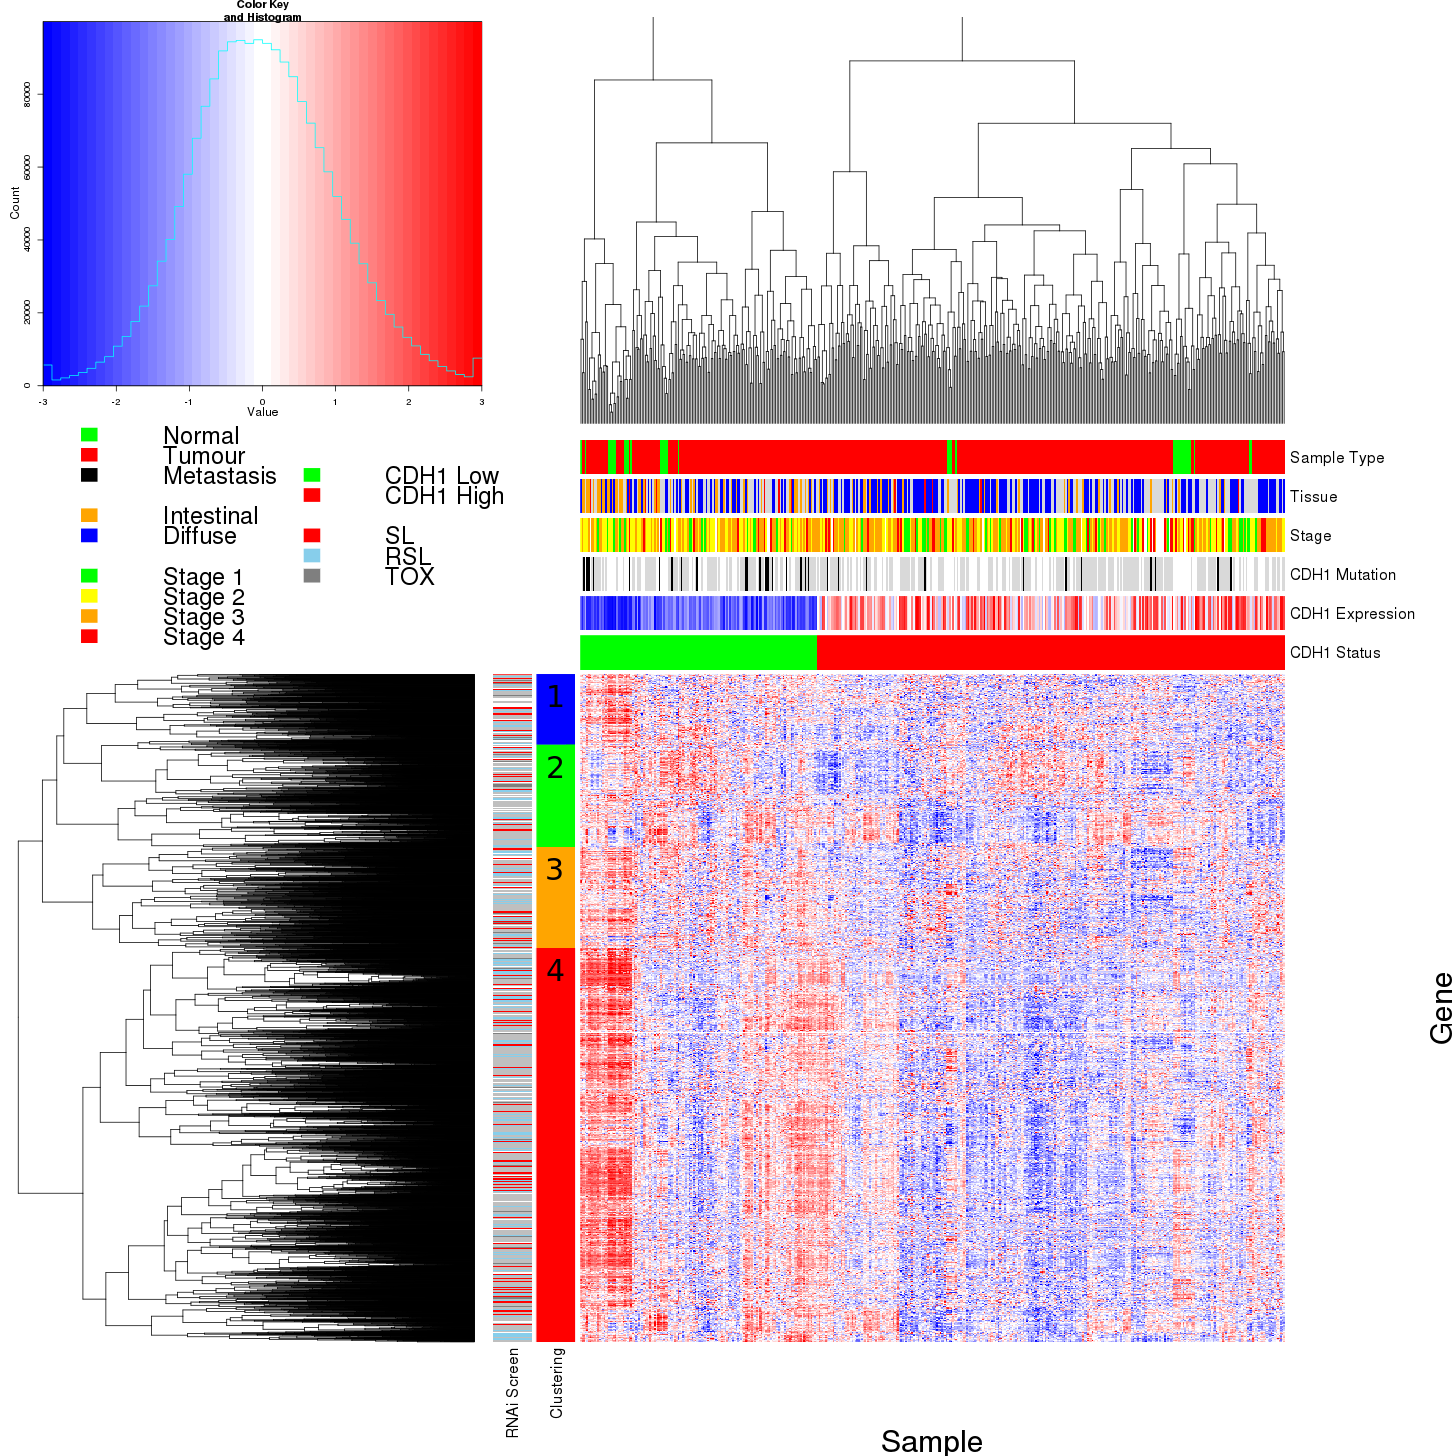
\includegraphics{CDH1_Heatmaps_Genes_Split_By_CDH1_z-trans_exprSL_cordistx_Pub_stad.png}
   }
    \caption[Synthetic lethal expression profiles of stomach samples]{\small \textbf{Synthetic lethal expression profiles of analysed samples.} Gene expression profile heatmap (correlation distance) of all samples (separated by the $\sfrac{1}{3}$ quantile of \textit{CDH1} expression) analysed in \gls{TCGA} stomach cancer dataset for gene expression of 4365 candidate partners of \gls{E-cadherin} (\textit{CDH1}) from \gls{SLIPT} prediction (with significant \gls{FDR} adjusted $p < 0.05$). Deeply clustered, inter-correlated genes form several main groups, each containing genes that were SL candidates or toxic in an \gls{siRNA} screen \cite{Telford2015}. Clusters had different sample groups highly expressing the synthetic lethal candidates in \textit{CDH1} low samples. Notably, diffuse and \textit{CDH1} mutant samples had elevated expression in one or more distinct clusters, although there was less complexity and variation among candidate synthetic lethal partners than in breast data. \textit{CDH1} low samples also contained most of samples with \textit{CDH1} mutations.
   %This suggests that multiple targets may be needed to target \textit{CDH1} deficiency across genetic backgrounds and that combination therapy may be more effective. 
}
\label{fig:slipt_expr_stad}
%\end{mdframed}
\end{figure*}

%The \gls{SLIPT} partners of \textit{CDH1} exhibited similar clustering in staomch cancer to breast cancer, replicating the diverse roles of elevated partner genes in different clinical samples. Specifically (in Figure~\ref{fig:slipt_expr_stad}), the diffuse type stomach cancers had higher expression of the candidate synthetic lethal partners (where \textit{CDH1} has a role as a driver mutation), despite an unbiased clustering. This is consistent with compensating expression of synthetic lethal partners under loss of \textit{CDH1}, as suggested by \citet{Lu2015}. The pathway composition of gene clusters for stomach cancer (shown in Table~\ref{tab:pathway_clusters_stad}) was also highly concordant with breast cancer findings (shown in Table~\ref{tab:pathway_clusters}). These included replicated of translation (Cluster 1), immune functions (Cluster 2), G$_{\alpha s}$ signalling (Cluster 3), and further support for the roles of GPCRs and the extracellular matrix (Cluster 4) in the synthetic lethal partners and functions of \textit{CDH1}, replicated across stomach and breast cancers. Clusters 1 and 4, which had particularly high expression of \gls{SLIPT} candidate partner genes in the diffuse subtype, also had the most significant over-representation of pathways.

%There was less variation between the expression profiles of \acrshort{mtSLIPT} partners of \textit{CDH1} in stomach cancer, although clusters were still detectable (as shown in Figure~\ref{fig:slipt_expr_stad_mtSL}). While the genes and pathways detected was lewss significant (due to lower sample size), the composition of clusters was further indicative for the roles of extracellular matrix (including elastic fibres), immune functions, and the cell signalling.


\begin{table*}[!hp]
\caption{Pathways for clusters of \textit{CDH1} partners in stomach SLIPT}
\label{tab:pathway_clusters_stad}
\centering
%\begin{tiny}
%\makebox[\textwidth][c]{
\resizebox{0.75 \textwidth}{!}{
\begin{threeparttable}
\begin{tabular}{lccc}
%\caption{Pathways for clusters of \textit{CDH1} partners from SLIPT}
%\label{tab:pathway_clusters}
  \large{\textbf{Pathways Over-represented in Cluster 1}} & \large{\textbf{Pathway Size}} & \large{\textbf{Cluster Genes}} & \large{\textbf{p-value (\gls{FDR})}} \\ %(833 genes)  
  \hline
  \rowcolor{Cluster_Blue!20}
  Viral \acrshort{mRNA} Translation &  82 &  48 & $1.3 \times 10^{-97}$ \\ 
  \rowcolor{Cluster_Blue!15}
  Formation of a pool of free 40S subunits &  94 &  51 & $1.3 \times 10^{-97}$ \\ 
  \rowcolor{Cluster_Blue!20}
  Eukaryotic Translation Elongation &  87 &  49 & $4.8 \times 10^{-97}$ \\ 
  \rowcolor{Cluster_Blue!15}
  Peptide chain elongation &  84 &  48 & $1.4 \times 10^{-96}$ \\ 
  \rowcolor{Cluster_Blue!20}
  Eukaryotic Translation Termination &  84 &  48 & $1.4 \times 10^{-96}$ \\ 
  \rowcolor{Cluster_Blue!15}
  GTP hydrolysis and joining of the 60S ribosomal subunit & 105 &  52 & $7.9 \times 10^{-94}$ \\ 
  \rowcolor{Cluster_Blue!20}
  Nonsense Mediated Decay independent of the Exon Junction Complex &  89 &  48 & $3.1 \times 10^{-93}$ \\ 
  \rowcolor{Cluster_Blue!15}
  L13a-mediated translational silencing of Ceruloplasmin expression & 104 &  51 & $5.1 \times 10^{-92}$ \\ 
  \rowcolor{Cluster_Blue!20}
  3' -UTR-mediated translational regulation & 104 &  51 & $5.1 \times 10^{-92}$ \\ 
  \rowcolor{Cluster_Blue!15}
  SRP-dependent cotranslational protein targeting to membrane & 105 &  51 & $1.7 \times 10^{-91}$ \\ 
  \rowcolor{Cluster_Blue!20}
  Eukaryotic Translation Initiation & 112 &  52 & $3.3 \times 10^{-90}$ \\ 
  \rowcolor{Cluster_Blue!15}
  Cap-dependent Translation Initiation & 112 &  52 & $3.3 \times 10^{-90}$ \\ 
  \rowcolor{Cluster_Blue!20}
  Translation & 142 &  56 & $3.6 \times 10^{-85}$ \\ 
  \rowcolor{Cluster_Blue!15}
  Nonsense-Mediated Decay & 104 &  48 & $1.2 \times 10^{-84}$ \\ 
  \rowcolor{Cluster_Blue!20}
  Nonsense Mediated Decay enhanced by the Exon Junction Complex & 104 &  48 & $1.2 \times 10^{-84}$ \\ 
  \rowcolor{Cluster_Blue!15}
  Influenza Viral \acrshort{RNA} Transcription and Replication & 109 &  48 & $4.1 \times 10^{-82}$ \\ 
  \rowcolor{Cluster_Blue!20}
  Influenza Life Cycle & 113 &  48 & $3.4 \times 10^{-80}$ \\ 
  \rowcolor{Cluster_Blue!15}
  Influenza Infection & 118 &  48 & $6.4 \times 10^{-78}$ \\ 
%  \rowcolor{Cluster_Blue!20}
%  Infectious disease & 349 &  68 & $1.8 \times 10^{-50}$ \\ 
%  \rowcolor{Cluster_Blue!15}
%  Formation of the ternary complex, and subsequently, the 43S complex &  48 &  21 & $3.7 \times 10^{-43}$ \\ 
  \hline
%  \\
  \cellcolor{white} \large{\textbf{Pathways Over-represented in Cluster 2}} & \large{\textbf{Pathway Size}} & \large{\textbf{Cluster Genes}} & \large{\textbf{p-value (\gls{FDR})}} \\ %(833 genes)  
  \hline
  \rowcolor{Cluster_Green!20}
  Immunoregulatory interactions between a Lymphoid and a non-Lymphoid cell &  65 &  12 & $1.3 \times 10^{-15}$ \\ 
  \rowcolor{Cluster_Green!15}
  Phosphorylation of CD3 and TCR zeta chains &  18 &   6 & $1.7 \times 10^{-12}$ \\ 
  \rowcolor{Cluster_Green!20}
  Generation of second messenger molecules &  29 &   7 & $2.7 \times 10^{-12}$ \\ 
  \rowcolor{Cluster_Green!15}
  PD-1 signalling &  21 & $  6 & 7.4 \times 10^{-12}$ \\ 
  \rowcolor{Cluster_Green!20}
  TCR signalling &  62 & $  9 & 4.3 \times 10^{-11}$ \\ 
  \rowcolor{Cluster_Green!15}
  Translocation of ZAP-70 to Immunological synapse &  16 & $  5 & 1.1 \times 10^{-10}$ \\ 
  \rowcolor{Cluster_Green!20}
  Interferon alpha/beta signalling &  68 & $  9 & 1.6 \times 10^{-10}$ \\ 
  \rowcolor{Cluster_Green!15}
  Initial triggering of complement &  17 & $  5 & 1.6 \times 10^{-10}$ \\ 
  \rowcolor{Cluster_Green!20}
  IKK complex recruitment mediated by RIP1 &  19 & $  5 & 5.1 \times 10^{-10}$ \\ 
  \rowcolor{Cluster_Green!15}
  TRIF-mediated programmed cell death &  10 & $  4 & 6.2 \times 10^{-10}$ \\ 
  \rowcolor{Cluster_Green!20}
  Creation of C4 and C2 activators &  11 & $  4 & 1.3 \times 10^{-9}$ \\ 
  \rowcolor{Cluster_Green!15}
  RHO GTPases Activate NADPH Oxidases &  11 & $  4 & 1.3 \times 10^{-9}$ \\ 
  \rowcolor{Cluster_Green!20}
  Interferon Signalling & 175 &  15 & $2.3 \times 10^{-9}$ \\ 
  \rowcolor{Cluster_Green!15}
  Chemokine receptors bind chemokines &  52 &   7 & $4.0 \times 10^{-9}$ \\ 
  \rowcolor{Cluster_Green!20}
  Interferon gamma signalling &  74 &   8 & $1.6 \times 10^{-8}$ \\ 
  \rowcolor{Cluster_Green!15}
  TRAF6 mediated induction of TAK1 complex &  15 &   4 & $1.6 \times 10^{-8}$ \\ 
  \rowcolor{Cluster_Green!20}
  Activation of IRF3/IRF7 mediated by TBK1/IKK epsilon &  16 &   4 & $2.7 \times 10^{-8}$ \\ 
  \rowcolor{Cluster_Green!15}
  Downstream TCR signalling &  45 &   6 & $3.5 \times 10^{-8}$ \\ 
%  \rowcolor{Cluster_Green!20}
%  Ligand-dependent caspase activation &  17 &   4 & $4.2 \times 10^{-8}$ \\ 
%  \rowcolor{Cluster_Green!15}
%  Complement cascade &  34 &   5 & $1.3 \times 10^{-7}$ \\ 
  \hline
%  \\
  \cellcolor{white} \large{\textbf{Pathways Over-represented in Cluster 3}} & \large{\textbf{Pathway Size}} & \large{\textbf{Cluster Genes}} & \large{\textbf{p-value (\gls{FDR})}} \\ %(833 genes)  
  \hline
  \rowcolor{Cluster_Orange!30}
  Uptake and actions of bacterial toxins &  22 &   4 & $3.5 \times 10^{-6}$ \\ 
  \rowcolor{Cluster_Orange!20}
  Neurotoxicity of clostridium toxins &  10 &   3 & $3.5 \times 10^{-6}$ \\ 
  \rowcolor{Cluster_Orange!30}
  Activation of PPARGC1A (PGC-1alpha) by phosphorylation &  10 &   3 & $3.5 \times 10^{-6}$ \\ 
  \rowcolor{Cluster_Orange!20}
  SMAD2/SMAD3:SMAD4 heterotrimer regulates transcription &  28 &   4 & $1.4 \times 10^{-5}$ \\ 
  \rowcolor{Cluster_Orange!30}
  Assembly of the primary cilium & 149 &  10 & $2.5 \times 10^{-5}$ \\ 
  \rowcolor{Cluster_Orange!20}
  Serotonin Neurotransmitter Release Cycle &  15 &   3 & $2.5 \times 10^{-5}$ \\ 
  \rowcolor{Cluster_Orange!30}
  Glycosaminoglycan metabolism & 114 &   8 & $3.3 \times 10^{-5}$ \\ 
  \rowcolor{Cluster_Orange!20}
  Platelet homeostasis &  54 &   5 & $3.3 \times 10^{-5}$ \\ 
  \rowcolor{Cluster_Orange!30}
  Norepinephrine Neurotransmitter Release Cycle &  17 &   3 & $3.3 \times 10^{-5}$ \\ 
  \rowcolor{Cluster_Orange!20}
  Acetylcholine Neurotransmitter Release Cycle &  17 &   3 & $3.3 \times 10^{-5}$ \\ 
  \rowcolor{Cluster_Orange!30}
  G$_{\alpha s}$ signalling events & 100 &   7 & $5.5 \times 10^{-5}$ \\ 
  \rowcolor{Cluster_Orange!20}
  GABA synthesis, release, reuptake and degradation &  19 &   3 & $5.6 \times 10^{-5}$ \\ 
  \rowcolor{Cluster_Orange!30}
  deactivation of the beta-catenin transactivating complex &  39 &   4 & $6.7 \times 10^{-5}$ \\ 
  \rowcolor{Cluster_Orange!20}
  Dopamine Neurotransmitter Release Cycle &  20 &   3 & $6.7 \times 10^{-5}$ \\ 
  \rowcolor{Cluster_Orange!30}
  IRS-related events triggered by IGF1R &  83 &   6 & $7.1 \times 10^{-5}$ \\ 
  \rowcolor{Cluster_Orange!20}
  Generic Transcription Pathway & 186 &  11 & $7.1 \times 10^{-5}$ \\ 
  \rowcolor{Cluster_Orange!30}
  Termination of O-glycan biosynthesis &  21 &   3 & $7.4 \times 10^{-5}$ \\ 
  \rowcolor{Cluster_Orange!20}
  Kinesins &  22 &   3 & $8.5 \times 10^{-5}$ \\ 
%  \rowcolor{Cluster_Orange!30}
%  Signalling by Type 1 Insulin-like Growth Factor 1 Receptor (IGF1R) &  86 &   6 & $8.5 \times 10^{-5}$ \\ 
%  \rowcolor{Cluster_Orange!20}
%  IGF1R signalling cascade &  86 &   6 & $8.5 \times 10^{-5}$ \\
  \hline
%  \\ 
  \cellcolor{white} \large{\textbf{Pathways Over-represented in Cluster 4}} & \large{\textbf{Pathway Size}} & \large{\textbf{Cluster Genes}} & \large{\textbf{p-value (\gls{FDR})}} \\ %(833 genes)  
  \hline 
  \rowcolor{Cluster_Red!20}
  Extracellular matrix organization & 241 &  97 & $8.8 \times 10^{-126}$ \\ 
  \rowcolor{Cluster_Red!15}
  Axon guidance & 289 &  75 & $8.3 \times 10^{-72}$ \\ 
  \rowcolor{Cluster_Red!20}
  Hemostasis & 445 & 101 & $8.3 \times 10^{-72}$ \\ 
  \rowcolor{Cluster_Red!15}
  Developmental Biology & 432 &  95 & $3.0 \times 10^{-67}$ \\ 
  \rowcolor{Cluster_Red!20}
  Response to elevated platelet cytosolic Ca$^{2+}$ &  84 &  37 & $5.8 \times 10^{-67}$ \\ 
  \rowcolor{Cluster_Red!15}
  Platelet degranulation &  79 &  36 & $5.8 \times 10^{-67}$ \\ 
  \rowcolor{Cluster_Red!20}
  Degradation of the extracellular matrix & 104 &  39 & $6.7 \times 10^{-63}$ \\ 
  \rowcolor{Cluster_Red!15}
  Platelet activation, signalling and aggregation & 186 &  52 & $6.6 \times 10^{-62}$ \\ 
  \rowcolor{Cluster_Red!20}
  ECM proteoglycans &  66 &  31 & $8.1 \times 10^{-61}$ \\ 
  \rowcolor{Cluster_Red!15}
  Neuronal System & 272 &  64 & $5.1 \times 10^{-60}$ \\ 
  \rowcolor{Cluster_Red!20}
  Signalling by PDGF & 173 &  47 & $9.7 \times 10^{-57}$ \\ 
  \rowcolor{Cluster_Red!15}
  Integrin cell surface interactions &  82 &  31 & $1.9 \times 10^{-53}$ \\ 
  \rowcolor{Cluster_Red!20}
  Collagen biosynthesis and modifying enzymes &  56 &  26 & $1.1 \times 10^{-52}$ \\ 
  \rowcolor{Cluster_Red!15}
  Collagen formation &  67 &  28 & $1.4 \times 10^{-52}$ \\ 
  \rowcolor{Cluster_Red!20}
  Class A/1 (Rhodopsin-like receptors) & 289 &  61 & $2.3 \times 10^{-52}$ \\ 
  \rowcolor{Cluster_Red!15}
  GPCR ligand binding & 373 &  73 & $2.8 \times 10^{-52}$ \\ 
  \rowcolor{Cluster_Red!20}
  Elastic fibre formation &  38 &  22 & $4.7 \times 10^{-52}$ \\ 
  \rowcolor{Cluster_Red!15}
  Non-integrin membrane-ECM interactions &  53 &  24 & $7.0 \times 10^{-49}$ \\ 
%  \rowcolor{Cluster_Red!20}
%  Glycosaminoglycan metabolism & 114 &  33 & $4.7 \times 10^{-47}$ \\ 
%  \rowcolor{Cluster_Red!15}
%  Platelet homeostasis &  54 &  23 & $1.0 \times 10^{-45}$ \\ 
 \hline
\end{tabular}
\begin{tablenotes}
\raggedright %\small
Pathway over-representation analysis for Reactome pathways with the number of genes in each pathway (Pathway Size), number of genes within the pathway identified (Cluster Genes), and the pathway over-representation p-value (adjusted by \gls{FDR}) from the hypergeometric test.  
\end{tablenotes}
\end{threeparttable}
}
\end{table*}

%%appendix
%\label{tab:pathway_clusters_stad_mtSL}

\FloatBarrier

\section{Comparison to Primary Screen} \label{appendix:compare_exprSL_genes_stad}

The synthetic lethal partners with \textit{CDH1} expression in stomach cancers were also compared to \gls{siRNA} primary screen data \citep{Telford2015}, as performed in Section~\ref{chapt3:primary_screen}. These were expected to be more concordant with the experimental results performed on a null mutant, however this was not the case at the gene level: less genes overlapped with experimental candidates in Figure~\ref{fig:Venn_allgenes_stad}. This may be due to lower sample size for mutations in \gls{TCGA} data or lower frequency (expected value) of \textit{CDH1} mutations compared to low expression. 



\begin{figure}[!ht]
%\begin{mdframed}
  \centering
  \resizebox{0.66 \columnwidth}{!}{
    \includegraphics{Venn_exprSL_siRNA_allgenes_reduced_Pub_stad.png}
   }
    \caption[Comparison of SLIPT in stomach to \gls{siRNA}]{\small \textbf{Comparison of SLIPT in stomach to \gls{siRNA}.} The overlap of gene candidates for \gls{E-cadherin} synthetic lethal partners between computational (SLIPT) and experimental screening (siRNA) approaches. The $\chi^2$ test suggests that the overlap is no more than would be expected by chance ($p = 0.281$). %A Venn diagram of all 16298 genes tested by both approaches.
}
\label{fig:Venn_allgenes_stad}
%\end{mdframed}
\end{figure}

%%appendix
%\label{fig:Venn_allgenes_stad_mtSL}

\FloatBarrier

\begin{table*}[!hp]
\caption{Pathways for \textit{CDH1} partners from SLIPT and \gls{siRNA}}
\label{tab:Venn_over-representation_stad}
\centering
\resizebox{0.8 \textwidth}{!}{
\begin{tabular}{sl^c^c^c}
\rowstyle{\bfseries}
  Predicted only by SLIPT (3392 genes) & Pathway Size & Genes Identified & p-value (\gls{FDR}) \\ 
  \hline
  \rowcolor{Cluster_Red!20}
  Extracellular matrix organization & 238 &  90 & $3.4 \times 10^{-107}$ \\ 
  \rowcolor{Cluster_Red!15}
  Eukaryotic Translation Termination &  79 &  46 & $7.6 \times 10^{-91}$ \\ 
  \rowcolor{Cluster_Red!20}
  Viral \acrshort{mRNA} Translation &  77 &  45 & $1.2 \times 10^{-89}$ \\ 
  \rowcolor{Cluster_Red!15}
  Eukaryotic Translation Elongation &  82 &  46 & $5.8 \times 10^{-89}$ \\ 
  \rowcolor{Cluster_Red!20}
  Peptide chain elongation &  79 &  45 & $2.1 \times 10^{-88}$ \\ 
  \rowcolor{Cluster_Red!15}
  Nonsense Mediated Decay independent of the Exon Junction Complex &  84 &  46 & $9.4 \times 10^{-88}$ \\ 
  \rowcolor{Cluster_Red!20}
  Formation of a pool of free 40S subunits &  89 &  47 & $3.3 \times 10^{-87}$ \\ 
  \rowcolor{Cluster_Red!15}
  GTP hydrolysis and joining of the 60S ribosomal subunit & 100 &  48 & $3.2 \times 10^{-83}$ \\ 
  \rowcolor{Cluster_Red!20}
  Axon guidance & 284 &  84 & $3.9 \times 10^{-82}$ \\ 
  \rowcolor{Cluster_Red!15}
  Developmental Biology & 426 & 111 & $4.2 \times 10^{-82}$ \\ 
  \rowcolor{Cluster_Red!20}
  L13a-mediated translational silencing of Ceruloplasmin expression &  99 &  47 & $1.4 \times 10^{-81}$ \\ 
  \rowcolor{Cluster_Red!15}
  3' -UTR-mediated translational regulation &  99 &  47 & $1.4 \times 10^{-81}$ \\ 
  \rowcolor{Cluster_Red!20}
  SRP-dependent cotranslational protein targeting to membrane &  99 &  47 & $1.4 \times 10^{-81}$ \\ 
  \rowcolor{Cluster_Red!15}
  Nonsense-Mediated Decay &  99 &  47 & $1.4 \times 10^{-81}$ \\ 
  \rowcolor{Cluster_Red!20}
  Nonsense Mediated Decay enhanced by the Exon Junction Complex &  99 &  47 & $1.4 \times 10^{-81}$ \\ 
  \rowcolor{Cluster_Red!15}
  Hemostasis & 438 & 112 & $1.2 \times 10^{-80}$ \\ 
  \rowcolor{Cluster_Red!20}
  Eukaryotic Translation Initiation & 107 &  48 & $8.0 \times 10^{-80}$ \\ 
  \rowcolor{Cluster_Red!15}
  Cap-dependent Translation Initiation & 107 &  48 & $8.0 \times 10^{-80}$ \\ 
  \rowcolor{Cluster_Red!20}
  Infectious disease & 338 &  90 & $1.6 \times 10^{-76}$ \\ 
  \rowcolor{Cluster_Red!15}
  Neuronal System & 267 &  77 & $1.6 \times 10^{-76}$ \\ 
  \hline
  \\
  \rowstyle{\bfseries}
  Detected only by \gls{siRNA} screen (1803 genes) & Pathway Size & Genes Identified & p-value (\gls{FDR}) \\ 
  \hline
  \rowcolor{Cluster_Blue!20}
  Class A/1 (Rhodopsin-like receptors) & 282 &  62 & $8.1 \times 10^{-50}$ \\ 
  \rowcolor{Cluster_Blue!15}
  GPCR ligand binding & 363 &  71 & $4.9 \times 10^{-46}$ \\ 
  \rowcolor{Cluster_Blue!20}
  Peptide ligand-binding receptors & 175 &  38 & $7.9 \times 10^{-38}$ \\ 
  \rowcolor{Cluster_Blue!15}
  G$_{\alpha i}$ signalling events & 184 &  37 & $1.1 \times 10^{-34}$ \\ 
  \rowcolor{Cluster_Blue!20}
  Gastrin-CREB signalling pathway via PKC and MAPK & 180 &  35 & $1.4 \times 10^{-32}$ \\ 
  \rowcolor{Cluster_Blue!15}
  G$_{\alpha q}$ signalling events & 159 &  32 & $4.8 \times 10^{-32}$ \\ 
  \rowcolor{Cluster_Blue!20}
  DAP12 interactions & 159 &  29 & $1.4 \times 10^{-27}$ \\ 
  \rowcolor{Cluster_Blue!15}
  Downstream signal transduction & 146 &  26 & $2.4 \times 10^{-25}$ \\ 
  \rowcolor{Cluster_Blue!20}
  DAP12 signalling & 149 &  26 & $6.4 \times 10^{-25}$ \\ 
  \rowcolor{Cluster_Blue!15}
  VEGFA-VEGFR2 Pathway &  91 &  19 & $8.1 \times 10^{-24}$ \\ 
  \rowcolor{Cluster_Blue!20}
  Signalling by PDGF & 172 &  27 & $5.7 \times 10^{-23}$ \\ 
  \rowcolor{Cluster_Blue!15}
  Signalling by ERBB2 & 146 &  24 & $1.4 \times 10^{-22}$ \\ 
  \rowcolor{Cluster_Blue!20}
  Signalling by VEGF &  99 &  19 & $2.0 \times 10^{-22}$ \\ 
  \rowcolor{Cluster_Blue!15}
  Visual phototransduction &  85 &  17 & $1.3 \times 10^{-21}$ \\ 
  \rowcolor{Cluster_Blue!20}
  Downstream signalling of activated FGFR1 & 134 &  22 & $1.3 \times 10^{-21}$ \\ 
  \rowcolor{Cluster_Blue!15}
  Downstream signalling of activated FGFR2 & 134 &  22 & $1.3 \times 10^{-21}$ \\ 
  \rowcolor{Cluster_Blue!20}
  Downstream signalling of activated FGFR3 & 134 &  22 & $1.3 \times 10^{-21}$ \\ 
  \rowcolor{Cluster_Blue!15}
  Downstream signalling of activated FGFR4 & 134 &  22 & $1.3 \times 10^{-21}$ \\ 
  \rowcolor{Cluster_Blue!20}
  Signalling by FGFR & 146 &  23 & $2.0 \times 10^{-21}$ \\ 
  \rowcolor{Cluster_Blue!15}
  Signalling by FGFR1 & 146 &  23 & $2.0 \times 10^{-21}$ \\ 
  \hline
  \\
  \rowstyle{\bfseries}
  Intersection of SLIPT and \gls{siRNA} screen (547 genes) & Pathway Size & Genes Identified & p-value (\gls{FDR}) \\ 
  \hline
  \rowcolor{Cluster_Red!20!Cluster_Blue!20}
  Class A/1 (Rhodopsin-like receptors) & 282 &  25 & $3.9 \times 10^{-9}$ \\ 
  \rowcolor{Cluster_Red!15!Cluster_Blue!15}
  Platelet activation, signalling and aggregation & 182 &  17 & $3.9 \times 10^{-9}$ \\ 
  \rowcolor{Cluster_Red!20!Cluster_Blue!20}
  Response to elevated platelet cytosolic Ca$2^+$ &  82 &   9 & $5.5 \times 10^{-8}$ \\ 
  \rowcolor{Cluster_Red!15!Cluster_Blue!15}
  Platelet homeostasis &  53 &   7 & $5.7 \times 10^{-8}$ \\ 
  \rowcolor{Cluster_Red!20!Cluster_Blue!20}
  Nucleotide-like (purinergic) receptors &  16 &   4 & $1.8 \times 10^{-7}$ \\ 
  \rowcolor{Cluster_Red!15!Cluster_Blue!15}
  Platelet degranulation &  77 &   8 & $2.8 \times 10^{-7}$ \\ 
  \rowcolor{Cluster_Red!20!Cluster_Blue!20}
  Peptide ligand-binding receptors & 175 &  14 & $3.8 \times 10^{-7}$ \\ 
  \rowcolor{Cluster_Red!15!Cluster_Blue!15}
  Molecules associated with elastic fibres &  34 &   5 & $7.1 \times 10^{-7}$ \\ 
  \rowcolor{Cluster_Red!20!Cluster_Blue!20}
  Amine ligand-binding receptors &  35 &   5 & $8.6 \times 10^{-7}$ \\ 
  \rowcolor{Cluster_Red!15!Cluster_Blue!15}
  G$_{\alpha i}$ signalling events & 184 &  14 & $9.8 \times 10^{-7}$ \\ 
  \rowcolor{Cluster_Red!20!Cluster_Blue!20}
  GPCR ligand binding & 363 &  27 & $1.1 \times 10^{-6}$ \\ 
  \rowcolor{Cluster_Red!15!Cluster_Blue!15}
  Elastic fibre formation &  38 &   5 & $1.5 \times 10^{-6}$ \\ 
  \rowcolor{Cluster_Red!20!Cluster_Blue!20}
  G$_{\alpha q}$ signalling events & 159 &  12 & $1.9 \times 10^{-6}$ \\ 
  \rowcolor{Cluster_Red!15!Cluster_Blue!15}
  Serotonin receptors &  12 &   3 & $3.8 \times 10^{-6}$ \\ 
  \rowcolor{Cluster_Red!20!Cluster_Blue!20}
  P2Y receptors &  12 &   3 & $3.8 \times 10^{-6}$ \\ 
  \rowcolor{Cluster_Red!15!Cluster_Blue!15}
  Signal amplification &  16 &   3 & $2.3 \times 10^{-5}$ \\ 
  \rowcolor{Cluster_Red!20!Cluster_Blue!20}
  Gastrin-CREB signalling pathway via PKC and MAPK & 180 &  12 & $2.3 \times 10^{-5}$ \\ 
  \rowcolor{Cluster_Red!15!Cluster_Blue!15}
  Complement cascade &  33 &   4 & $2.4 \times 10^{-5}$ \\ 
  \rowcolor{Cluster_Red!20!Cluster_Blue!20}
  Glycosaminoglycan metabolism & 110 &   8 & $2.5 \times 10^{-5}$ \\ 
  \rowcolor{Cluster_Red!15!Cluster_Blue!15}
  Glycogen breakdown (glycogenolysis) &  17 &   3 & $2.7 \times 10^{-5}$ \\ 
  \hline
\end{tabular}
}
\end{table*}



%%appendix
%\label{tab:Venn_over-representation_stad_mtSL}



\FloatBarrier

\subsection{Resampling Analysis}  \label{appendix:compare_pathway_perm_stad_exprSL}


%For replication of resampling in stomach cancer, 1 million iterations were used to estimate the permutation p-value.

\begin{table*}[!htp]
\caption{Pathways for \textit{CDH1} partners from SLIPT in stomach cancer}
\label{tab:pathway_perm_stad}
\centering
\resizebox{0.8 \textwidth}{!}{
\begin{threeparttable}
\begin{tabular}{sl^c^c}
\rowstyle{\bfseries}
  Reactome Pathway & Over-representation & Permutation \\ 
  \hline
  \rowcolor{Cluster_Red!20} 
  \textit{Extracellular matrix organization} & $7.5 \times 10^{-140}$ & $0.070215$ \\ 
  \rowcolor{Cluster_Red!15} 
  Hemostasis & $1.8 \times 10^{-121}$ & $0.25804$ \\ 
  \rowcolor{Cluster_Red!20} 
  Developmental Biology & $9.2 \times 10^{-107}$ & $0.53032$ \\ 
  \rowcolor{Cluster_Red!15} 
  Axon guidance & $1.5 \times 10^{-102}$ & $0.6704$ \\ 
  \rowcolor{Cluster_Red!20} 
  \textbf{Eukaryotic Translation Termination} & $1.9 \times 10^{-99}$ & $>1.031 \times 10^{-5}$ \\ 
  \rowcolor{Cluster_Red!15} 
  GPCR ligand binding & $3.8 \times 10^{-99}$ & $0.54914$ \\ 
  \rowcolor{Cluster_Red!20} 
  \textbf{Viral \acrshort{mRNA} Translation} & $3.3 \times 10^{-98}$ & $>1.031 \times 10^{-5}$ \\ 
  \rowcolor{Cluster_Red!15} 
  \textbf{Formation of a pool of free 40S subunits} & $3.3 \times 10^{-98}$ & $>1.031 \times 10^{-5}$ \\ 
  \rowcolor{Cluster_Red!20} 
  \textbf{Eukaryotic Translation Elongation} & $1.6 \times 10^{-97}$ & $>1.031 \times 10^{-5}$ \\ 
  \rowcolor{Cluster_Red!15} 
  \textbf{Peptide chain elongation} & $7.2 \times 10^{-97}$ & $>1.031 \times 10^{-5}$ \\ 
  \rowcolor{Cluster_Red!20} 
  Class A/1 (Rhodopsin-like receptors) & $2.7 \times 10^{-96}$ & $0.58174$ \\ 
  \rowcolor{Cluster_Red!15} 
  \textbf{Nonsense Mediated Decay independent of the Exon Junction Complex} & $3 \times 10^{-96}$ & $>1.031 \times 10^{-5}$ \\ 
  \rowcolor{Cluster_Red!20} 
  Infectious disease & $2.6 \times 10^{-94}$ & $0.25484$ \\ 
  \rowcolor{Cluster_Red!15} 
  \textbf{GTP hydrolysis and joining of the 60S ribosomal subunit} & $3.4 \times 10^{-94}$ & $>1.031 \times 10^{-5}$ \\ 
  \rowcolor{Cluster_Red!20} 
  \textbf{L13a-mediated translational silencing of Ceruloplasmin expression} & $2.8 \times 10^{-92}$ & $>1.031 \times 10^{-5}$ \\ 
  \rowcolor{Cluster_Red!15} 
  \textbf{3' -UTR-mediated translational regulation} & $2.8 \times 10^{-92}$ & $>1.031 \times 10^{-5}$ \\ 
  \rowcolor{Cluster_Red!20} 
  Neuronal System & $8.4 \times 10^{-92}$ & $0.53433$ \\ 
  \rowcolor{Cluster_Red!15} 
  \textbf{SRP-dependent cotranslational protein targeting to membrane} & $9.5 \times 10^{-92}$ & $>1.031 \times 10^{-5}$ \\ 
  \rowcolor{Cluster_Red!20} 
  \textbf{Eukaryotic Translation Initiation} & $2.0 \times 10^{-90}$ & $>1.031 \times 10^{-5}$ \\ 
  \rowcolor{Cluster_Red!15} 
  \textbf{Cap-dependent Translation Initiation} & $2.0 \times 10^{-90}$ & $>1.031 \times 10^{-5}$ \\ 
  \rowcolor{Cluster_Red!20} 
  \textbf{Nonsense-Mediated Decay} & $7.4 \times 10^{-90}$ & $>1.031 \times 10^{-5}$ \\ 
  \rowcolor{Cluster_Red!15} 
  \textbf{Nonsense Mediated Decay enhanced by the Exon Junction Complex} & $7.4 \times 10^{-90}$ & $>1.031 \times 10^{-5}$ \\ 
  \rowcolor{Cluster_Red!20} 
  Adaptive Immune System & $8.1 \times 10^{-88}$ & $0.14116$ \\ 
  \rowcolor{Cluster_Red!15} 
  \textbf{Translation} & $1.3 \times 10^{-87}$ & $>1.031 \times 10^{-5}$ \\ 
  \rowcolor{Cluster_Red!20} 
  Platelet activation, signalling and aggregation & $1.3 \times 10^{-86}$ & $0.28959$ \\ 
  \rowcolor{Cluster_Red!15} 
  \textbf{Influenza Infection} & $1 \times 10^{-82}$ & $>1.031 \times 10^{-5}$ \\ 
  \rowcolor{Cluster_Red!20} 
  \textbf{Influenza Viral \acrshort{RNA} Transcription and Replication} & $2.4 \times 10^{-82}$ & $>1.031 \times 10^{-5}$ \\ 
  \rowcolor{Cluster_Red!15} 
  \textbf{Influenza Life Cycle} & $2 \times 10^{-80}$ & $>1.031 \times 10^{-5}$ \\ 
  \rowcolor{Cluster_Red!20} 
  Response to elevated platelet cytosolic Ca$2^+$ & $4.9 \times 10^{-78}$ & $0.50817$ \\ 
  \rowcolor{Cluster_Red!15} 
  Signalling by NGF & $1.6 \times 10^{-75}$ & $0.38518$ \\ 
  \rowcolor{Cluster_Red!20} 
  Rho GTPase cycle & $5.1 \times 10^{-75}$ & $0.14864$ \\ 
  \rowcolor{Cluster_Red!15} 
  Signalling by PDGF & $7.4 \times 10^{-74}$ & $0.40493$ \\ 
  \rowcolor{Cluster_Red!20} 
  \textit{Signalling by Rho GTPases} & $5.1 \times 10^{-73}$ & $0.077217$ \\ 
  \rowcolor{Cluster_Red!15} 
  Glycosaminoglycan metabolism & $1.4 \times 10^{-68}$ & $0.52984$ \\ 
  \rowcolor{Cluster_Red!20} 
  G$_{\alpha i}$ signalling events & $1.8 \times 10^{-66}$ & $0.9254$ \\ 
  \rowcolor{Cluster_Red!15} 
  Metabolism of carbohydrates & $1.1 \times 10^{-65}$ & $0.39501$ \\ 
  \rowcolor{Cluster_Red!20} 
  \textbf{G$_{\alpha s}$ signalling events} & $2.7 \times 10^{-65}$ & $0.0050293$ \\ 
  \rowcolor{Cluster_Red!15} 
  Potassium Channels & $2.7 \times 10^{-65}$ & $0.53359$ \\ 
  \rowcolor{Cluster_Red!20} 
  Transmission across Chemical Synapses & $1.8 \times 10^{-64}$ & $0.81833$ \\ 
  \rowcolor{Cluster_Red!15} 
  ECM proteoglycans & $3.4 \times 10^{-64}$ & $0.083482$ \\ 
  \rowcolor{Cluster_Red!20} 
  Peptide ligand-binding receptors & $4.8 \times 10^{-64}$ & $0.62817$ \\ 
  \rowcolor{Cluster_Red!15} 
  Degradation of the extracellular matrix & $1.1 \times 10^{-63}$ & $0.80879$ \\ 
  \rowcolor{Cluster_Red!20} 
  Platelet homeostasis & $5.3 \times 10^{-63}$ & $0.53134$ \\ 
  \rowcolor{Cluster_Red!15} 
  NGF signalling via TRKA from the plasma membrane & $6.1 \times 10^{-63}$ & $0.5717$ \\ 
  \rowcolor{Cluster_Red!20} 
  Integration of energy metabolism & $4.5 \times 10^{-61}$ & $0.10889$ \\ 
  \rowcolor{Cluster_Red!15} 
  Collagen formation & $5.4 \times 10^{-61}$ & $0.29896$ \\ 
  \rowcolor{Cluster_Red!20} 
  Integrin cell surface interactions & $7 \times 10^{-59}$ & $0.18167$ \\ 
  \rowcolor{Cluster_Red!15} 
  Collagen biosynthesis and modifying enzymes & $7 \times 10^{-59}$ & $0.30208$ \\ 
  \rowcolor{Cluster_Red!20} 
  \begin{tabular}[c]{@{}l@{}}Neurotransmitter Receptor Binding And Downstream Transmission\\ In The  Postsynaptic Cell \end{tabular} & $8.7 \times 10^{-57}$ & $0.82522$ \\ 
  \rowcolor{Cluster_Red!15} 
  Signalling by Wnt & $8.7 \times 10^{-57}$ & $0.25468$ \\ 
 \hline
\end{tabular}
\begin{tablenotes}
\raggedright \small
Over-representation (hypergeometric test) and Permutation p-values adjusted for multiple tests across pathways (\gls{FDR}). Significant pathways were marked in bold (\gls{FDR} $ < 0.05$) and italics (\gls{FDR} $ < 0.1$).
\end{tablenotes}
\end{threeparttable}
}
\end{table*}


\begin{table*}[!htp]
\caption{Pathways for \textit{CDH1} partners from SLIPT in stomach and \gls{siRNA}}
\label{tab:pathway_perm_overlap_stad}
\centering
\resizebox{0.8 \textwidth}{!}{
\begin{threeparttable}
\begin{tabular}{sl^c^c}
\rowstyle{\bfseries}
  Reactome Pathway & Over-representation & Permutation \\ 
  \hline
  \rowcolor{Cluster_Red!20!Cluster_Blue!20} 
  Platelet activation, signalling and aggregation & $3.9 \times 10^{-9}$ & $0.49557$ \\ 
  \rowcolor{Cluster_Red!15!Cluster_Blue!15} 
  Class A/1 (Rhodopsin-like receptors) & $3.9 \times 10^{-9}$ & $0.98432$ \\ 
  \rowcolor{Cluster_Red!20!Cluster_Blue!20} 
  Response to elevated platelet cytosolic Ca$2^+$ & $5.5 \times 10^{-8}$ & $0.54349$ \\ 
  \rowcolor{Cluster_Red!15!Cluster_Blue!15} 
  Platelet homeostasis & $5.7 \times 10^{-8}$ & $0.45017$ \\ 
  \rowcolor{Cluster_Red!20!Cluster_Blue!20} 
  Nucleotide-like (purinergic) receptors & $1.8 \times 10^{-7}$ & $0.36966$ \\ 
  \rowcolor{Cluster_Red!15!Cluster_Blue!15} 
  Peptide ligand-binding receptors & $3.8 \times 10^{-7}$ & $0.91294$ \\ 
  \rowcolor{Cluster_Red!20!Cluster_Blue!20} 
  \textbf{Molecules associated with elastic fibres} & $7.1 \times 10^{-7}$ & $0.0025868$ \\ 
  \rowcolor{Cluster_Red!15!Cluster_Blue!15} 
  Amine ligand-binding receptors & $8.6 \times 10^{-7}$ & $0.43303$ \\ 
  \rowcolor{Cluster_Red!20!Cluster_Blue!20} 
  G$_{\alpha i}$ signalling events & $9.8 \times 10^{-7}$ & $0.99626$ \\ 
  \rowcolor{Cluster_Red!15!Cluster_Blue!15} 
  GPCR ligand binding & $1.1 \times 10^{-6}$ & $0.97733$ \\ 
  \rowcolor{Cluster_Red!20!Cluster_Blue!20} 
  \textbf{Elastic fibre formation} & $1.5 \times 10^{-6}$ & $0.0025868$ \\ 
  \rowcolor{Cluster_Red!15!Cluster_Blue!15} 
  G$_{\alpha q}$ signalling events & $1.9 \times 10^{-6}$ & $0.86089$ \\ 
  \rowcolor{Cluster_Red!20!Cluster_Blue!20} 
  P2Y receptors & $3.8 \times 10^{-6}$ & $0.18795$ \\ 
  \rowcolor{Cluster_Red!15!Cluster_Blue!15} 
  Serotonin receptors & $3.8 \times 10^{-6}$ & $0.37853$ \\ 
  \rowcolor{Cluster_Red!20!Cluster_Blue!20} 
  Signal amplification & $2.3 \times 10^{-5}$ & $0.47856$ \\ 
  \rowcolor{Cluster_Red!15!Cluster_Blue!15} 
  Gastrin-CREB signalling pathway via PKC and MAPK & $2.3 \times 10^{-5}$ & $0.98567$ \\ 
  \rowcolor{Cluster_Red!20!Cluster_Blue!20} 
  \textbf{Complement cascade} & $2.4 \times 10^{-5}$ & $>3.4628 \times 10^{-6}$ \\ 
  \rowcolor{Cluster_Red!15!Cluster_Blue!15} 
  Glycosaminoglycan metabolism & $2.5 \times 10^{-5}$ & $0.38953$ \\ 
  \rowcolor{Cluster_Red!20!Cluster_Blue!20} 
  Glycogen breakdown (glycogenolysis) & $2.7 \times 10^{-5}$ & $0.83772$ \\ 
  \rowcolor{Cluster_Red!15!Cluster_Blue!15} 
  Defective B4GALT7 causes EDS, progeroid type & $4.9 \times 10^{-5}$ & $0.10792$ \\ 
  \rowcolor{Cluster_Red!20!Cluster_Blue!20} 
  Defective B3GAT3 causes JDSSDHD & $4.9 \times 10^{-5}$ & $0.10792$ \\ 
  \rowcolor{Cluster_Red!15!Cluster_Blue!15} 
  Role of LAT2/NTAL/LAB on calcium mobilization & $5.6 \times 10^{-5}$ & $0.35373$ \\ 
  \rowcolor{Cluster_Red!20!Cluster_Blue!20} 
  Cell surface interactions at the vascular wall & $5.6 \times 10^{-5}$ & $0.47642$ \\ 
  \rowcolor{Cluster_Red!15!Cluster_Blue!15} 
  \textbf{G$_{\alpha s}$ signalling events} & $6 \times 10^{-5}$ & $0.019858$ \\ 
  \rowcolor{Cluster_Red!20!Cluster_Blue!20} 
  Signalling by NOTCH & $6 \times 10^{-5}$ & $0.19008$ \\ 
  \rowcolor{Cluster_Red!15!Cluster_Blue!15} 
  A tetrasaccharide linker sequence is required for GAG synthesis & $0.00017$ & $0.47642$ \\ 
  \rowcolor{Cluster_Red!20!Cluster_Blue!20} 
  \textbf{Extracellular matrix organization} & $0.00018$ & $0.0047308$ \\ 
  \rowcolor{Cluster_Red!15!Cluster_Blue!15} 
  Collagen formation & $0.00018$ & $0.19245$ \\ 
  \rowcolor{Cluster_Red!20!Cluster_Blue!20} 
  Effects of PIP2 hydrolysis & $0.0002$ & $0.37779$ \\ 
  \rowcolor{Cluster_Red!15!Cluster_Blue!15} 
  Syndecan interactions & $0.0002$ & $0.37779$ \\ 
  \rowcolor{Cluster_Red!20!Cluster_Blue!20} 
  \textbf{Diseases associated with glycosaminoglycan metabolism} & $0.00023$ & $0.01028$ \\ 
  \rowcolor{Cluster_Red!15!Cluster_Blue!15} 
  \textbf{Diseases of glycosylation} & $0.00023$ & $0.01028$ \\ 
  \rowcolor{Cluster_Red!20!Cluster_Blue!20} 
  \textit{Chondroitin sulfate/dermatan sulfate metabolism} & $0.00023$ & $0.085541$ \\ 
  \rowcolor{Cluster_Red!15!Cluster_Blue!15} 
  Integrin alphaIIb beta3 signalling & $0.00028$ & $0.76936$ \\ 
  \rowcolor{Cluster_Red!20!Cluster_Blue!20} 
  Keratan sulfate biosynthesis & $0.00034$ & $0.68744$ \\ 
  \rowcolor{Cluster_Red!15!Cluster_Blue!15} 
  Rho GTPase cycle & $0.00034$ & $0.15675$ \\ 
  \rowcolor{Cluster_Red!20!Cluster_Blue!20} 
  Creation of C4 and C2 activators & $0.00035$ & $0.12275$ \\ 
  \rowcolor{Cluster_Red!15!Cluster_Blue!15} 
  Abacavir transport and metabolism & $0.00035$ & $0.12443$ \\ 
  \rowcolor{Cluster_Red!20!Cluster_Blue!20} 
  Amine compound SLC transporters & $0.00037$ & $0.69773$ \\ 
  \rowcolor{Cluster_Red!15!Cluster_Blue!15} 
  FCERI mediated NF-kB activation & $0.00037$ & $0.69846$ \\ 
  \rowcolor{Cluster_Red!20!Cluster_Blue!20} 
  Fc epsilon receptor (FCERI) signalling & $0.00056$ & $0.43303$ \\ 
  \rowcolor{Cluster_Red!15!Cluster_Blue!15} 
  Defective EXT2 causes exostoses 2 & $0.00067$ & $0.16053$ \\ 
  \rowcolor{Cluster_Red!20!Cluster_Blue!20} 
  Defective EXT1 causes exostoses 1, TRPS2 and CHDS & $0.00067$ & $0.16053$ \\ 
  \rowcolor{Cluster_Red!15!Cluster_Blue!15} 
  \textit{Collagen biosynthesis and modifying enzymes} & $0.00071$ & $0.052911$ \\ 
  \rowcolor{Cluster_Red!20!Cluster_Blue!20} 
  Keratan sulfate/keratin metabolism & $0.00073$ & $0.46533$ \\ 
  \rowcolor{Cluster_Red!15!Cluster_Blue!15} 
  G alpha (12/13) signalling events & $0.00078$ & $0.59164$ \\ 
  \rowcolor{Cluster_Red!20!Cluster_Blue!20} 
  \textbf{SEMA3A-Plexin repulsion signalling by inhibiting Integrin adhesion} & $0.00084$ & $0.038504$ \\ 
  \rowcolor{Cluster_Red!15!Cluster_Blue!15} 
  Signal attenuation & $0.00084$ & $0.37779$ \\ 
  \rowcolor{Cluster_Red!20!Cluster_Blue!20} 
  Eicosanoid ligand-binding receptors & $0.0011$ & $0.11117$ \\ 
  \rowcolor{Cluster_Red!15!Cluster_Blue!15} 
  SOS-mediated signalling & $0.0011$ & $0.25387$ \\ 
  \hline
\end{tabular}
\begin{tablenotes}
\raggedright \small
Over-representation (hypergeometric test) and Permutation p-values adjusted for multiple tests across pathways (\gls{FDR}). Significant pathways were marked in bold (\gls{FDR} $ < 0.05$) and italics (\gls{FDR} $ < 0.1$).
\end{tablenotes}
\end{threeparttable}
}
\end{table*}  

%%appendix
%\label{tab:pathway_perm_stad_mtSL}}
%\label{tab:pathway_perm_overlap_stad_mtSL}


\FloatBarrier

\section{Metagene Analysis} \label{appendix:metagene_stad_exprSL}

Metagenes used to detect synthetic lethal pathways with \textit{CDH1} in stomach cancer.% These were described and compared to mutation analysis in Section~\ref{appendix:metagene_stad_mtSL}. 

\begin{table*}[!ht]
\caption{Synthetic lethal metagenes against \textit{CDH1} in stomach cancer}
\label{tab:metagene_stad_SL}
\centering
\resizebox{1 \textwidth}{!}{
\begin{threeparttable}
\begin{tabular}{sl^l^c^c^c^c^c}
\rowstyle{\bfseries}
 Pathway & ID & Observed & Expected & $\chi^2$value & p-value & p-value (\gls{FDR}) \\
  \hline
  \rowcolor{black!10}
  Cell-Cell communication & 1500931 & 18 & 50.4 & 110 & $7.43 \times 10^{-23}$ & $1.53 \times 10^{-20}$ \\ 
  \rowcolor{black!5}
  VEGFR2 mediated vascular permeability & 5218920 & 19 & 50.4 & 109 & $1.36 \times 10^{-22}$ & $2.49 \times 10^{-20}$ \\ 
  \rowcolor{black!10}
  Sema4D in semaphorin signalling & 400685 & 20 & 50.4 & 104 & $1.62 \times 10^{-21}$ & $2.12 \times 10^{-19}$ \\ 
  \rowcolor{black!5}
  Ion transport by P-type ATPases & 936837 & 17 & 50.4 & 100 & $8.29 \times 10^{-21}$ & $8.06 \times 10^{-19}$ \\ 
  \rowcolor{black!10}
  Sialic acid metabolism & 4085001 & 19 & 50.4 & 95.3 & $9.95 \times 10^{-20}$ & $7.82 \times 10^{-18}$ \\ 
  \rowcolor{black!5}
  Synthesis of pyrophosphates in the cytosol & 1855167 & 26 & 50.4 & 94 & $1.86 \times 10^{-19}$ & $1.23 \times 10^{-17}$ \\ 
  \rowcolor{black!10}
  Keratan sulfate/keratin metabolism & 1638074 & 25 & 50.4 & 93.5 & $2.36 \times 10^{-19}$ & $1.44 \times 10^{-17}$ \\ 
  \rowcolor{black!5}
  Ion channel transport & 983712 & 19 & 50.4 & 92.8 & $3.37 \times 10^{-19}$ & $1.99 \times 10^{-17}$ \\ 
  \rowcolor{black!10}
  Keratan sulfate biosynthesis & 2022854 & 26 & 50.4 & 91.4 & $6.79 \times 10^{-19}$ & $3.62 \times 10^{-17}$ \\ 
  \rowcolor{black!5}
  Arachidonic acid metabolism & 2142753 & 22 & 50.4 & 90.6 & $9.81 \times 10^{-19}$ & $5.07 \times 10^{-17}$ \\ 
  \rowcolor{black!10}
  RHO GTPases activate CIT & 5625900 & 22 & 50.4 & 87 & $5.80 \times 10^{-18}$ & $2.66 \times 10^{-16}$ \\ 
  \rowcolor{black!5}
  Stimuli-sensing channels & 2672351 & 25 & 50.4 & 85.8 & $1.03 \times 10^{-17}$ & $4.58 \times 10^{-16}$ \\ 
  \rowcolor{black!10}
  Synthesis of PI & 1483226 & 19 & 50.4 & 85.6 & $1.15 \times 10^{-17}$ & $4.89 \times 10^{-16}$ \\ 
  \rowcolor{black!5}
  G-protein activation & 202040 & 19 & 50.4 & 85.3 & $1.34 \times 10^{-17}$ & $5.53 \times 10^{-16}$ \\ 
  \rowcolor{black!10}
  NrCAM interactions & 447038 & 22 & 50.4 & 84.3 & $2.1 \times 10^{-17}$ & $8.27 \times 10^{-16}$ \\ 
  \rowcolor{black!5}
  Inwardly rectifying $K^+$ channels & 1296065 & 24 & 50.4 & 83.5 & $3.19 \times 10^{-17}$ & $1.22 \times 10^{-15}$ \\ 
  \rowcolor{black!10}
  Calcitonin-like ligand receptors & 419812 & 20 & 50.4 & 82.2 & $6.07 \times 10^{-17}$ & $2.13 \times 10^{-15}$ \\ 
  \rowcolor{black!5}
  Prostacyclin signalling through prostacyclin receptor & 392851 & 24 & 50.4 & 81.8 & $7.27 \times 10^{-17}$ & $2.5 \times 10^{-15}$ \\ 
  \rowcolor{black!10}
  Presynaptic function of Kainate receptors & 500657 & 26 & 50.4 & 79.7 & $2.00 \times 10^{-16}$ & $6.34 \times 10^{-15}$ \\ 
  \rowcolor{black!5}
  ADP signalling through P2Y purinoceptor 12 & 392170 & 23 & 50.4 & 79.2 & $2.57 \times 10^{-16}$ & $7.71 \times 10^{-15}$ \\ 
  \rowcolor{black!10}
  regulation of FZD by ubiquitination & 4641263 & 22 & 50.4 & 78.8 & $3.15 \times 10^{-16}$ & $9.3 \times 10^{-15}$ \\ 
  \rowcolor{black!5}
  Toxicity of tetanus toxin (TeNT) & 5250982 & 27 & 50.4 & 78.7 & $3.36 \times 10^{-16}$ & $9.75 \times 10^{-15}$ \\ 
  \rowcolor{black!10}
  Gap junction degradation & 190873 & 21 & 50.4 & 78.5 & $3.66 \times 10^{-16}$ & $1.04 \times 10^{-14}$ \\ 
  \rowcolor{black!5}
  Nephrin interactions & 373753 & 25 & 50.4 & 78.2 & $4.21 \times 10^{-16}$ & $1.14 \times 10^{-14}$ \\ 
  \rowcolor{black!10}
  GABA synthesis, release, reuptake and degradation & 888590 & 26 & 50.4 & 77 & $7.69 \times 10^{-16}$ & $1.95 \times 10^{-14}$ \\ 
  \hline
\end{tabular}
\begin{tablenotes}
\raggedright \small
Strongest candidate \gls{synthetic lethal} partners for \textit{CDH1} by SLIPT with observed and expected numbers of \gls{TCGA} stomach cancer samples with low expression of both genes.
\end{tablenotes}
\end{threeparttable}
}
\end{table*}


\FloatBarrier

\iffalse
\chapter{Stomach Mutation Analysis}
\label{appendix:stad_mtSL}

The following results were a replication of the \gls{TCGA} results (in Appendix~\ref{appendix:mtSL}) with stomach cancer data, using synthetic lethality (\acrshort{mtSLIPT}) against \textit{CDH1} mutation.

\section{Synthetic Lethal Genes and Pathways} \label{appendix:stad_mtSL_genes}

\begin{table*}[!ht]
\caption{Synthetic lethal gene partners of \textit{CDH1} from \acrshort{mtSLIPT} in stomach cancer}
\label{tab:gene_stad_mtSL}
\centering
\resizebox{0.8 \textwidth}{!}{
\begin{threeparttable}
\begin{tabular}{>{\em}sl^c^c^c^c^c}
\rowstyle{\bfseries}
 \em{Gene} & Observed\tnote{*}  & Expected\tnote{*} & $\chi^2$ value & p-value & p-value (\gls{FDR}) \\ 
  \hline
  \rowcolor{black!10}
  OLFML1 & 5 & 10.1 & 29.2 & $4.53 \times 10^{-7}$ & $0.0031$ \\ 
  \rowcolor{black!5}
  NRIP2 & 6 & 10.1 & 25.4 & $3.11 \times 10^{-6}$ & $0.00706$ \\ 
  \rowcolor{black!10}
  VIM & 3 & 10.1 & 24.7 & $4.29 \times 10^{-6}$ & $0.00706$ \\ 
  \rowcolor{black!5}
  TCF4 & 5 & 10.1 & 24.7 & $4.33 \times 10^{-6}$ & $0.00706$ \\ 
  \rowcolor{black!10}
  ZEB2 & 5 & 10.1 & 24.7 & $4.33 \times 10^{-6}$ & $0.00706$ \\ 
  \rowcolor{black!5}
  BCL2 & 2 & 10.1 & 22 & $1.66 \times 10^{-5}$ & $0.0155$ \\ 
  \rowcolor{black!10}
  SMARCA2 & 2 & 10.1 & 22 & $1.66 \times 10^{-5}$ & $0.0155$ \\ 
  \rowcolor{black!5}
  CCND2 & 3 & 10.1 & 21.1 & $2.61 \times 10^{-5}$ & $0.0155$ \\ 
  \rowcolor{black!10}
  MMP19 & 3 & 10.1 & 21.1 & $2.61 \times 10^{-5}$ & $0.0155$ \\ 
  \rowcolor{black!5}
  NEURL1B & 3 & 10.1 & 21.1 & $2.61 \times 10^{-5}$ & $0.0155$ \\ 
  \rowcolor{black!10}
  IGFBP6 & 6 & 10.1 & 21.1 & $2.65 \times 10^{-5}$ & $0.0155$ \\ 
  \rowcolor{black!5}
  OGN & 6 & 10.1 & 21.1 & $2.65 \times 10^{-5}$ & $0.0155$ \\ 
  \rowcolor{black!10}
  THY1 & 6 & 10.2 & 21 & $2.7 \times 10^{-5}$ & $0.0155$ \\ 
  \rowcolor{black!5}
  DZIP1 & 4 & 10.1 & 20.6 & $3.29 \times 10^{-5}$ & $0.0155$ \\ 
  \rowcolor{black!10}
  LOC650368 & 4 & 10.1 & 20.6 & $3.29 \times 10^{-5}$ & $0.0155$ \\ 
  \rowcolor{black!5}
  PCOLCE & 4 & 10.1 & 20.6 & $3.29 \times 10^{-5}$ & $0.0155$ \\ 
  \rowcolor{black!10}
  PTGFR & 4 & 10.1 & 20.6 & $3.29 \times 10^{-5}$ & $0.0155$ \\ 
  \rowcolor{black!5}
  RUNX1T1 & 4 & 10.1 & 20.6 & $3.29 \times 10^{-5}$ & $0.0155$ \\ 
  \rowcolor{black!10}
  CLEC2B & 5 & 10.1 & 20.6 & $3.3 \times 10^{-5}$ & $0.0155$ \\ 
  \rowcolor{black!5}
  MSC & 5 & 10.1 & 20.6 & $3.3 \times 10^{-5}$ & $0.0155$ \\ 
  \rowcolor{black!10}
  NISCH & 5 & 10.1 & 20.6 & $3.3 \times 10^{-5}$ & $0.0155$ \\ 
  \rowcolor{black!5}
  TSPAN11 & 5 & 10.1 & 20.6 & $3.3 \times 10^{-5}$ & $0.0155$ \\ 
  \rowcolor{black!10}
  KCTD12 & 2 & 10.1 & 19.1 & $7.19 \times 10^{-5}$ & $0.0246$ \\ 
  \rowcolor{black!5}
  LRRC55 & 2 & 10.1 & 19.1 & $7.19 \times 10^{-5}$ & $0.0246$ \\ 
  \rowcolor{black!10}
  PCBP3 & 2 & 10.1 & 19.1 & $7.19 \times 10^{-5}$ & $0.0246$ \\
   \hline
\end{tabular}
\begin{tablenotes}
\raggedright \small
Strongest candidate \gls{synthetic lethal} partners for \textit{CDH1} by \acrshort{mtSLIPT} in \gls{TCGA} in stomach cancer expression and mutation data

\item[*] Observed and expected numbers of \textit{CDH1} mutant \gls{TCGA} stomach tumours with low expression of partner genes

\end{tablenotes}
\end{threeparttable}
}
\end{table*}

\FloatBarrier

\begin{table*}[!ht]
\caption{Pathways for \textit{CDH1} partners from \acrshort{mtSLIPT} in stomach cancer}
\label{tab:pathway_stad_mtSL}
\centering
\resizebox{1 \textwidth}{!}{
\begin{threeparttable}
\begin{tabular}{lccc}
 \textbf{Pathways Over-represented} & \textbf{Pathway Size} & \textbf{SL Genes} & \textbf{p-value (\gls{FDR})} \\
  \hline
  \rowcolor{black!10}
  Extracellular matrix organization & 241 &  20 & $9.6 \times 10^{-9}$ \\ 
  \rowcolor{black!5}
  Elastic fibre formation &  38 &   6 & $3.7 \times 10^{-8}$ \\ 
  \rowcolor{black!10}
  Diseases associated with glycosaminoglycan metabolism &  26 &   5 & $3.7 \times 10^{-8}$ \\ 
  \rowcolor{black!5}
  Diseases of glycosylation &  26 &   5 & $3.7 \times 10^{-8}$ \\ 
  \rowcolor{black!10}
  Nitric oxide stimulates guanylate cyclase &  24 &   4 & $3.1 \times 10^{-6}$ \\ 
  \rowcolor{black!5}
  Molecules associated with elastic fibres &  34 &   4 & $3.7 \times 10^{-5}$ \\ 
  \rowcolor{black!10}
  Platelet homeostasis &  54 &   5 & $3.7 \times 10^{-5}$ \\ 
  \rowcolor{black!5}
  Initial triggering of complement &  17 &   3 & $3.7 \times 10^{-5}$ \\ 
  \rowcolor{black!10}
  %Regulation of Insulin-like Growth Factor (IGF) transport and uptake by Insulin-like Growth Factor Binding Proteins (IGFBPs) &  17 &   3 & $3.7 \times 10^{-5}$ \\ 
  Regulation of IGF transport and uptake by IGFBPs &  17 &   3 & $3.7 \times 10^{-5}$ \\ 
  \rowcolor{black!5}
  Collagen degradation &  58 &   5 & $5.6 \times 10^{-5}$ \\ 
  \rowcolor{black!10}
  Defective B4GALT7 causes EDS, progeroid type &  19 &   3 & $5.6 \times 10^{-5}$ \\ 
  \rowcolor{black!5}
  Defective B3GAT3 causes JDSSDHD &  19 &   3 & $5.6 \times 10^{-5}$ \\ 
  \rowcolor{black!10}
  Degradation of the extracellular matrix & 104 &   7 & $8.0 \times 10^{-5}$ \\ 
  \rowcolor{black!5}
  ECM proteoglycans &  66 &   5 & 0.00017 \\ 
  \rowcolor{black!10}
  A tetrasaccharide linker sequence is required for GAG synthesis \textcolor{black!10}{x} &  25 &   3 & 0.00025 \\ 
  \rowcolor{black!5}
  RHO GTPases Activate WASPs and WAVEs &  29 &   3 & 0.00059 \\ 
  \rowcolor{black!10}
  Non-integrin membrane-ECM interactions &  53 &   4 & 0.00065 \\ 
  \rowcolor{black!5}
  Creation of C4 and C2 activators &  11 &   2 & 0.00079 \\ 
  \rowcolor{black!10}
  Dermatan sulfate biosynthesis &  11 &   2 & 0.00079 \\ 
  \rowcolor{black!5}
  Integrin cell surface interactions &  82 &   5 & 0.00098 \\ 
  \hline
\end{tabular}
\begin{tablenotes}
\raggedright \small
Gene set over-representation analysis (hypergeometric test) for Reactome pathways in \acrshort{mtSLIPT} partners for \textit{CDH1}.
\end{tablenotes}
\end{threeparttable}
}
\end{table*}


\FloatBarrier

%\clearpage
\section{Synthetic Lethal Expression Profiles} \label{appendix:stad_mtSL_clusters}

Similar to the analysis of synthetic lethal partners against low \textit{CDH1} expression in~\ref{appendix:stad_exprSL_genes}, the partners detected from \textit{CDH1} mutation were also examined for their expression profiles and the pathway composition of gene clusters. Hierachical clustering was performed on \acrshort{mtSLIPT} partners for \textit{CDH1} as showing in Figure~\ref{fig:slipt_expr_stad_mtSL}. Over-representation for Reactome pathways for each of the gene clusters identified is given in Table~\ref{tab:pathway_clusters_stad_mtSL}.


\begin{figure*}[!ht]
%\begin{mdframed}
  \centering
  \resizebox{0.99 \textwidth}{!}{
    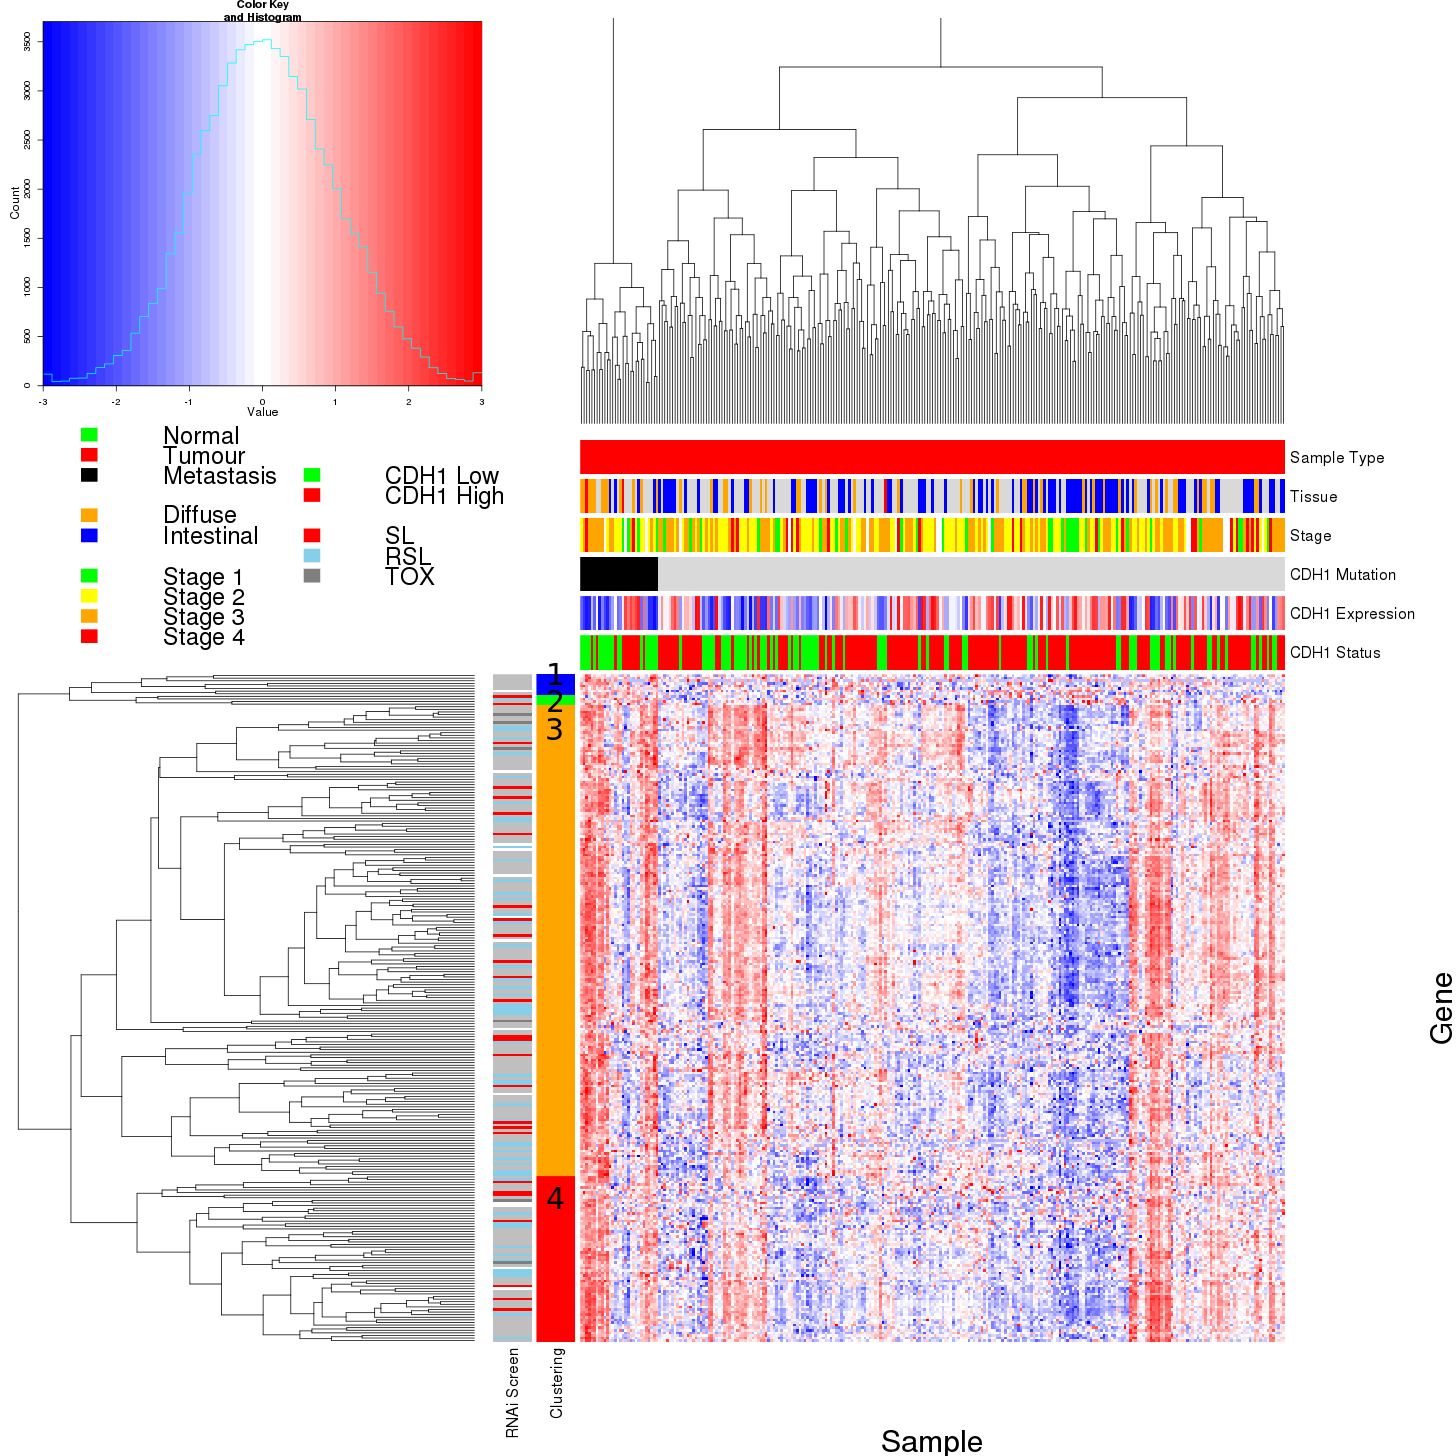
\includegraphics{CDH1_Heatmaps_Genes_Split_By_CDH1_z-trans_mtSL_cordistx_Pub_stad.png}
   }
    \caption[Synthetic lethal expression profiles of stomach samples]{\small \textbf{Synthetic lethal expression profiles of analysed samples.} Gene expression profile heatmap (correlation distance) of all samples (separated by the $\sfrac{1}{3}$ quantile of \textit{CDH1} expression) analysed in \gls{TCGA} stomach cancer dataset for gene expression of 257 candidate partners of \gls{E-cadherin} (\textit{CDH1}) from \gls{SLIPT} prediction (with significant \gls{FDR} adjusted $p < 0.05$). Deeply clustered, inter-correlated genes form several main groups, each containing genes that were SL candidates or toxic in an \gls{siRNA} screen \citep{Telford2015}. Clusters had different sample groups highly expressing the synthetic lethal candidates in \textit{CDH1} low samples. Notably, diffuse and \textit{CDH1} mutant samples had elevated expression in one or more distinct clusters, although there was less complexity and variation among candidate synthetic lethal partners than in breast data. \textit{CDH1} low samples also contained most of samples with \textit{CDH1} mutations.
   %This suggests that multiple targets may be needed to target \textit{CDH1} deficiency across genetic backgrounds and that combination therapy may be more effective. 
}
\label{fig:slipt_expr_stad_mtSL}
%\end{mdframed}
\end{figure*}

\FloatBarrier


\begin{table*}[!hp]
\caption{Pathways for clusters of \textit{CDH1} partners in stomach mtSLIPT}
\label{tab:pathway_clusters_stad_mtSL}
\centering
%\begin{tiny}
%\makebox[\textwidth][c]{
\resizebox{0.75 \textwidth}{!}{
\begin{threeparttable}
\begin{tabular}{lccc}
%\caption{Pathways for clusters of \textit{CDH1} partners from SLIPT}
%\label{tab:pathway_clusters_stad_mtSL}
  \large{\textbf{Pathways Over-represented in Cluster 1}} & \large{\textbf{Pathway Size}} & \large{\textbf{Cluster Genes}} & \large{\textbf{p-value (\gls{FDR})}} \\ %(833 genes)  
  \hline
  \rowcolor{Cluster_Blue!20}
  CD28 dependent PI3K/Akt signalling &  15 &   1 &   1 \\ 
  \rowcolor{Cluster_Blue!15}
  Hormone-sensitive lipase (HSL)-mediated triacylglycerol hydrolysis &  19 &   1 &   1 \\ 
  \rowcolor{Cluster_Blue!20}
  CD28 co-stimulation &  26 &   1 &   1 \\ 
  \rowcolor{Cluster_Blue!15}
  Lipid digestion, mobilization, and transport &  48 &   1 &   1 \\ 
  \rowcolor{Cluster_Blue!20}
  Costimulation by the CD28 family &  51 &   1 &   1 \\ 
  \rowcolor{Cluster_Blue!15}
  Dectin-1 mediated noncanonical NF-kB signalling &  58 &   1 &   1 \\ 
  \rowcolor{Cluster_Blue!20}
  CLEC7A (Dectin-1) signalling &  99 &   1 &   1 \\ 
  \rowcolor{Cluster_Blue!15}
  C-type lectin receptors (CLRs) & 123 &   1 &   1 \\ 
  \rowcolor{Cluster_Blue!20}
  Adaptive Immune System & 418 &   1 &   1 \\ 
  \rowcolor{Cluster_Blue!15}
  Metabolism of lipids and lipoproteins & 494 &   1 &   1 \\ 
  \rowcolor{Cluster_Blue!20}
  Interleukin-6 signalling &  10 &   0 &   1 \\ 
  \rowcolor{Cluster_Blue!15}
  Apoptosis & 150 &   0 &   1 \\ 
  \rowcolor{Cluster_Blue!20}
  Hemostasis & 445 &   0 &   1 \\ 
  \rowcolor{Cluster_Blue!15}
  Intrinsic Pathway for Apoptosis &  36 &   0 &   1 \\ 
  \rowcolor{Cluster_Blue!20}
  Cleavage of Growing Transcript in the Termination Region &  33 &   0 &   1 \\ 
  \rowcolor{Cluster_Blue!15}
  PKB-mediated events &  28 &   0 &   1 \\ 
  \rowcolor{Cluster_Blue!20}
  PI3K Cascade &  68 &   0 &   1 \\ 
  \rowcolor{Cluster_Blue!15}
  RAF/MAP kinase cascade &  10 &   0 &   1 \\ 
%  \rowcolor{Cluster_Blue!20}
%  Global \Gls{genomic} NER (GG-NER) &  35 &   0 &   1 \\ 
%  \rowcolor{Cluster_Blue!15}
%  Repair synthesis for gap-filling by \acrshort{DNA} polymerase in TC-NER &  15 &   0 &   1 \\ 
  \hline
%  \\
  \cellcolor{white} \large{\textbf{Pathways Over-represented in Cluster 2}} & \large{\textbf{Pathway Size}} & \large{\textbf{Cluster Genes}} & \large{\textbf{p-value (\gls{FDR})}} \\ %(833 genes)  
  \hline
  \rowcolor{Cluster_Green!30}
  Kinesins &  22 &   1 &   1 \\ 
  \rowcolor{Cluster_Green!20}
  O-linked glycosylation of mucins &  49 &   1 &   1 \\ 
  \rowcolor{Cluster_Green!30}
  O-linked glycosylation &  59 &   1 &   1 \\ 
  \rowcolor{Cluster_Green!20}
  MHC class II antigen presentation &  85 &   1 &   1 \\ 
  \rowcolor{Cluster_Green!30}
  Factors involved in megakaryocyte development and platelet production \textcolor{Cluster_Green!30} {cellll} & 120 &   1 &   1 \\
  \rowcolor{Cluster_Green!20}
  Post-translational protein modification & 303 &   1 &   1 \\ 
  \rowcolor{Cluster_Green!30}
  Adaptive Immune System & 418 &   1 &   1 \\ 
  \rowcolor{Cluster_Green!20}
  Hemostasis & 445 &   1 &   1 \\ 
  \rowcolor{Cluster_Green!30}
  Interleukin-6 signalling &  10 &   0 &   1 \\ 
  \rowcolor{Cluster_Green!20}
  Apoptosis & 150 &   0 &   1 \\ 
  \rowcolor{Cluster_Green!30}
  Intrinsic Pathway for Apoptosis &  36 &   0 &   1 \\ 
  \rowcolor{Cluster_Green!20}
  Cleavage of Growing Transcript in the Termination Region &  33 &   0 &   1 \\ 
  \rowcolor{Cluster_Green!30}
  PKB-mediated events &  28 &   0 &   1 \\ 
  \rowcolor{Cluster_Green!20}
  PI3K Cascade &  68 &   0 &   1 \\ 
  \rowcolor{Cluster_Green!30}
  RAF/MAP kinase cascade &  10 &   0 &   1 \\ 
  \rowcolor{Cluster_Green!20}
  Global \Gls{genomic} NER (GG-NER) &  35 &   0 &   1 \\ 
  \rowcolor{Cluster_Green!30}
  Repair synthesis for gap-filling by \acrshort{DNA} polymerase in TC-NER &  15 &   0 &   1 \\ 
  \rowcolor{Cluster_Green!20}
  Gap-filling \acrshort{DNA} repair synthesis and ligation in TC-NER &  17 &   0 &   1 \\ 
%  \rowcolor{Cluster_Green!30}
%  Formation of transcription-coupled NER (TC-NER) repair complex &  29 &   0 &   1 \\ 
%  \rowcolor{Cluster_Green!20}
%  Dual incision reaction in TC-NER &  29 &   0 &   1 \\ 
  \hline
%  \\ 
  \cellcolor{white} \large{\textbf{Pathways Over-represented in Cluster 3}} & \large{\textbf{Pathway Size}} & \large{\textbf{Cluster Genes}} & \large{\textbf{p-value (\gls{FDR})}} \\ %(833 genes)  
  \hline 
  \rowcolor{Cluster_Orange!20}
  Extracellular matrix organization & 241 &  20 & $9.6 \times 10^{-9}$ \\ 
  \rowcolor{Cluster_Orange!15}
  Elastic fibre formation &  38 &   6 & $3.7 \times 10^{-8}$ \\ 
  \rowcolor{Cluster_Orange!20}
  Diseases associated with glycosaminoglycan metabolism &  26 &   5 & $3.7 \times 10^{-8}$ \\ 
  \rowcolor{Cluster_Orange!15}
  Diseases of glycosylation &  26 &   5 & $3.7 \times 10^{-8}$ \\ 
  \rowcolor{Cluster_Orange!20}
  Molecules associated with elastic fibres &  34 &   4 & $4.8 \times 10^{-5}$ \\ 
  \rowcolor{Cluster_Orange!15}
  Initial triggering of complement &  17 &   3 & $4.8 \times 10^{-5}$ \\ 
  \rowcolor{Cluster_Orange!20}
  %\begin{tabular}[c]{@{}l@{}}Regulation of Insulin-like Growth Factor (IGF) transport and \\ uptake by Insulin-like Growth Factor Binding Proteins (IGFBPs)\end{tabular} &  17 &   3 & $4.8 \times 10^{-5}$ \\
  \begin{tabular}[c]{@{}l@{}}Regulation of  IGF transport and uptake by IGFBPs\end{tabular} &  17 &   3 & $4.8 \times 10^{-5}$ \\ 
  \rowcolor{Cluster_Orange!15}
  Collagen degradation &  58 &   5 & $6.7 \times 10^{-5}$ \\ 
  \rowcolor{Cluster_Orange!20}
  Defective B4GALT7 causes EDS, progeroid type &  19 &   3 & $6.7 \times 10^{-5}$ \\ 
  \rowcolor{Cluster_Orange!15}
  Defective B3GAT3 causes JDSSDHD &  19 &   3 & $6.7 \times 10^{-5}$ \\ 
  \rowcolor{Cluster_Orange!20}
  Degradation of the extracellular matrix & 104 &   7 & $9.5 \times 10^{-5}$ \\ 
  \rowcolor{Cluster_Orange!15}
  ECM proteoglycans &  66 &   5 & 0.0002 \\ 
  \rowcolor{Cluster_Orange!20}
  A tetrasaccharide linker sequence is required for GAG synthesis &  25 & 5 3 & 0.00029 \\ 
  \rowcolor{Cluster_Orange!15}
  Non-integrin membrane-ECM interactions &  53 &   4 & 0.00079 \\ 
  \rowcolor{Cluster_Orange!20}
  Creation of C4 and C2 activators &  11 &   2 & 0.00093 \\ 
  \rowcolor{Cluster_Orange!15}
  Dermatan sulfate biosynthesis &  11 &   2 & 0.00093 \\ 
  \rowcolor{Cluster_Orange!20}
  Integrin cell surface interactions &  82 &   5 & 0.0012 \\ 
  \rowcolor{Cluster_Orange!15}
  Keratan sulfate degradation &  12 &   2 & 0.0012 \\ 
%  \rowcolor{Cluster_Orange!20}
%  Complement cascade &  34 &   3 & 0.0013 \\ 
%  \rowcolor{Cluster_Orange!15}
%  CS/DS degradation &  13 &   2 & 0.0015 \\ 
  \hline
%  \\ 
  \cellcolor{white} \large{\textbf{Pathways Over-represented in Cluster 4}} & \large{\textbf{Pathway Size}} & \large{\textbf{Cluster Genes}} & \large{\textbf{p-value (\gls{FDR})}} \\ %(833 genes)  
  \hline
  \rowcolor{Cluster_Red!20}
  cGMP effects &  18 &   2 & 0.11 \\ 
  \rowcolor{Cluster_Red!15}
  Nitric oxide stimulates guanylate cyclase &  24 &   2 & 0.19 \\ 
  \rowcolor{Cluster_Red!20}
  Neurotoxicity of clostridium toxins &  10 &   1 &   1 \\ 
  \rowcolor{Cluster_Red!15}
  Platelet homeostasis &  54 &   2 &   1 \\ 
  \rowcolor{Cluster_Red!20}
  Eicosanoid ligand-binding receptors &  14 &   1 &   1 \\ 
  \rowcolor{Cluster_Red!15}
  Prolactin receptor signalling &  15 &   1 &   1 \\ 
  \rowcolor{Cluster_Red!20}
  Acyl chain remodelling of PI &  15 &   1 &   1 \\ 
  \rowcolor{Cluster_Red!15}
  Signalling by FGFR1 fusion mutants &  15 &   1 &   1 \\ 
  \rowcolor{Cluster_Red!20}
  PKA activation &  16 &   1 &   1 \\ 
  \rowcolor{Cluster_Red!15}
  PKA-mediated phosphorylation of CREB &  17 &   1 &   1 \\ 
  \rowcolor{Cluster_Red!20}
  Synthesis of glycosylphosphatidylinositol (GPI) &  17 &   1 &   1 \\ 
  \rowcolor{Cluster_Red!15}
  PKA activation in glucagon signalling &  17 &   1 &   1 \\ 
  \rowcolor{Cluster_Red!20}
  Butyrate Response Factor 1 (BRF1) destabilizes \acrshort{mRNA} &  17 &   1 &   1 \\ 
  \rowcolor{Cluster_Red!15}
  Other semaphorin interactions &  19 &   1 &   1 \\ 
  \rowcolor{Cluster_Red!20}
  Acyl chain remodelling of PE &  21 &   1 &   1 \\ 
  \rowcolor{Cluster_Red!15}
  Signalling by Leptin &  21 &   1 &   1 \\ 
  \rowcolor{Cluster_Red!20}
  DARPP-32 events &  22 &   1 &   1 \\ 
  \rowcolor{Cluster_Red!15}
  Glucagon-like Peptide-1 (GLP1) regulates insulin secretion &  22 &   1 &   1 \\ 
%  \rowcolor{Cluster_Red!20}
%  Uptake and actions of bacterial toxins &  22 &   1 &   1 \\ 
%  \rowcolor{Cluster_Red!15}
%  Acyl chain remodelling of PC &  23 &   1 &   1 \\ 
  \hline
\end{tabular}
\begin{tablenotes}
\raggedright %\small
Pathway over-representation analysis for Reactome pathways with the number of genes in each pathway (Pathway Size), number of genes within the pathway identified (Cluster Genes), and the pathway over-representation p-value (adjusted by \gls{FDR}) from the hypergeometric test.  
\end{tablenotes}
\end{threeparttable}
}
\end{table*}

\FloatBarrier

\section{Comparison to Primary Screen} \label{appendix:compare_mtSL_genes_stad}

The mutation synthetic lethal partners with \textit{CDH1} were also compared to \gls{siRNA} primary screen data \citep{Telford2015}, as performed in Section~\ref{chapt3:primary_screen}. These were expected to be more concordant with the experimental results performed on a null mutant, however this not the case at the gene level: less genes overlapped with experimental candidates in Figure~\ref{fig:Venn_allgenes_stad_mtSL}. This may be affected by lower sample size for mutations in \gls{TCGA} data or lower frequency (expected value) of \textit{CDH1} mutations compared to low expression. 

\begin{figure}[!ht]
%\begin{mdframed}
  \centering
  \resizebox{0.66 \columnwidth}{!}{
    \includegraphics{Venn_mtSL_siRNA_allgenes_reduced_Pub_stad.png}
   }
    \caption[Comparison of \acrshort{mtSLIPT} in stomach to \gls{siRNA}]{\small \textbf{Comparison of \acrshort{mtSLIPT} in stomach to \gls{siRNA}.} Testing the overlap of gene candidates for \gls{E-cadherin} synthetic lethal partners between computational (\acrshort{mtSLIPT}) and experimental screening (siRNA) approaches. The $\chi^2$ test suggests that the overlap is no more than would be expected by chance ($p = 0.872$). %A Venn diagram of all 16298 genes tested by both approaches.
}
\label{fig:Venn_allgenes_stad_mtSL}
%\end{mdframed}
\end{figure}


\begin{table*}[!hp]
\caption{Pathways for \textit{CDH1} partners from \acrshort{mtSLIPT} and \gls{siRNA}}
\label{tab:Venn_over-representation_stad_mtSL}
\centering
\resizebox{0.8 \textwidth}{!}{
\begin{tabular}{sl^c^c^c}
\rowstyle{\bfseries}
  Predicted only by SLIPT (217 genes) & Pathway Size & Genes Identified & p-value (\gls{FDR}) \\ 
  \hline
  \rowcolor{Cluster_Red!20}
  Diseases associated with glycosaminoglycan metabolism &  26 &   5 & $1.6 \times 10^{-7}$ \\ 
  \rowcolor{Cluster_Red!15}
  Diseases of glycosylation &  26 &   5 & $1.6 \times 10^{-7}$ \\ 
  \rowcolor{Cluster_Red!20}
  Extracellular matrix organization & 238 &  18 & $1.7 \times 10^{-6}$ \\ 
  \rowcolor{Cluster_Red!15}
  Elastic fibre formation &  38 &   5 & $4.6 \times 10^{-6}$ \\ 
  \rowcolor{Cluster_Red!20}
  Initial triggering of complement &  16 &   3 & $7.3 \times 10^{-5}$ \\ 
  \rowcolor{Cluster_Red!15}
  Regulation of IGF transport and uptake by IGFBPs &  17 &   3 & $8.9 \times 10^{-5}$ \\ 
  \rowcolor{Cluster_Red!20}
  Defective B4GALT7 causes EDS, progeroid type &  19 &   3 & $0.00013$ \\ 
  \rowcolor{Cluster_Red!15}
  Defective B3GAT3 causes JDSSDHD &  19 &   3 & $0.00013$ \\ 
  \rowcolor{Cluster_Red!20}
  Collagen degradation &  57 &   5 & $0.00013$ \\ 
  \rowcolor{Cluster_Red!15}
  ECM proteoglycans &  65 &   5 & $0.00039$ \\ 
  \rowcolor{Cluster_Red!20}
  A tetrasaccharide linker sequence is required for GAG synthesis &  24 &   3 & $0.00039$ \\ 
  \rowcolor{Cluster_Red!15}
  Nitric oxide stimulates guanylate cyclase &  24 &   3 & $0.00039$ \\ 
  \rowcolor{Cluster_Red!20}
  RHO GTPases Activate WASPs and WAVEs &  28 &   3 & $0.00094$ \\ 
  \rowcolor{Cluster_Red!15}
  Creation of C4 and C2 activators &  10 &   2 & $0.00098$ \\ 
  \rowcolor{Cluster_Red!20}
  Non-integrin membrane-ECM interactions &  52 &   4 & $0.0012$ \\ 
  \rowcolor{Cluster_Red!15}
  Dermatan sulfate biosynthesis &  11 &   2 & $0.0013$ \\ 
  \rowcolor{Cluster_Red!20}
  Degradation of the extracellular matrix & 101 &   6 & $0.0016$ \\ 
  \rowcolor{Cluster_Red!15}
  Keratan sulfate degradation &  12 &   2 & $0.0016$ \\ 
  \rowcolor{Cluster_Red!20}
  Complement cascade &  33 &   3 & $0.0018$ \\ 
  \rowcolor{Cluster_Red!15}
  Molecules associated with elastic fibres &  34 &   3 & $0.002$ \\ 
  \hline
  \\
  \rowstyle{\bfseries}
  Detected only by \gls{siRNA} screen (2323 genes) & Pathway Size & Genes Identified & p-value (\gls{FDR}) \\ 
  \hline
  \rowcolor{Cluster_Blue!20}
  Class A/1 (Rhodopsin-like receptors) & 282 &  86 & $6.5 \times 10^{-85}$ \\ 
  \rowcolor{Cluster_Blue!15}
  GPCR ligand binding & 363 &  97 & $9.2 \times 10^{-79}$ \\ 
  \rowcolor{Cluster_Blue!20}
  Peptide ligand-binding receptors & 175 &  52 & $4.5 \times 10^{-61}$ \\ 
  \rowcolor{Cluster_Blue!15}
  G$_{\alpha i}$ signalling events & 184 &  49 & $1.6 \times 10^{-53}$ \\ 
  \rowcolor{Cluster_Blue!20}
  G$_{\alpha q}$  signalling events & 159 &  43 & $5.2 \times 10^{-50}$ \\ 
  \rowcolor{Cluster_Blue!15}
  Gastrin-CREB signalling pathway via PKC and MAPK & 180 &  46 & $9.4 \times 10^{-50}$ \\ 
  \rowcolor{Cluster_Blue!20}
  DAP12 interactions & 159 &  35 & $8.3 \times 10^{-37}$ \\ 
  \rowcolor{Cluster_Blue!15}
  Platelet activation, signalling and aggregation & 182 &  37 & $2.3 \times 10^{-35}$ \\ 
  \rowcolor{Cluster_Blue!20}
  Hemostasis & 438 &  71 & $3.3 \times 10^{-35}$ \\ 
  \rowcolor{Cluster_Blue!15}
  Downstream signal transduction & 146 &  32 & $7.7 \times 10^{-35}$ \\ 
  \rowcolor{Cluster_Blue!20}
  Signalling by PDGF & 172 &  35 & $2.1 \times 10^{-34}$ \\ 
  \rowcolor{Cluster_Blue!15}
  DAP12 signalling & 149 &  32 & $2.7 \times 10^{-34}$ \\ 
  \rowcolor{Cluster_Blue!20}
  Signalling by ERBB2 & 146 &  31 & $2.5 \times 10^{-33}$ \\ 
  \rowcolor{Cluster_Blue!15}
  Signalling by NGF & 266 &  44 & $5.3 \times 10^{-31}$ \\ 
  \rowcolor{Cluster_Blue!20}
  Downstream signalling of activated FGFR1 & 134 &  28 & $5.3 \times 10^{-31}$ \\ 
  \rowcolor{Cluster_Blue!15}
  Downstream signalling of activated FGFR2 & 134 &  28 & $5.3 \times 10^{-31}$ \\ 
  \rowcolor{Cluster_Blue!20}
  Downstream signalling of activated FGFR3 & 134 &  28 & $5.3 \times 10^{-31}$ \\ 
  \rowcolor{Cluster_Blue!15}
  Downstream signalling of activated FGFR4 & 134 &  28 & $5.3 \times 10^{-31}$ \\ 
  \rowcolor{Cluster_Blue!20}
  Signalling by FGFR & 146 &  29 & $2.0 \times 10^{-30}$ \\ 
  \rowcolor{Cluster_Blue!15}
  Signalling by FGFR1 & 146 &  29 & $2.0 \times 10^{-30}$ \\ 
  \hline
  \\
  \rowstyle{\bfseries}
  Intersection of SLIPT and \gls{siRNA} screen (23 genes) & Pathway Size & Genes Identified & p-value (\gls{FDR}) \\ 
  \hline
  \rowcolor{Cluster_Red!20!Cluster_Blue!20}
  ADP signalling through P2Y purinoceptor 1 &  10 &   1 &   1 \\ 
  \rowcolor{Cluster_Red!15!Cluster_Blue!15}
  G-protein beta:gamma signalling &  11 &   1 &   1 \\ 
  \rowcolor{Cluster_Red!20!Cluster_Blue!20}
  G-protein activation &  12 &   1 &   1 \\ 
  \rowcolor{Cluster_Red!15!Cluster_Blue!15}
  Eicosanoid ligand-binding receptors &  14 &   1 &   1 \\ 
  \rowcolor{Cluster_Red!20!Cluster_Blue!20}
  Platelet homeostasis &  53 &   2 &   1 \\ 
  \rowcolor{Cluster_Red!15!Cluster_Blue!15}
  G$_{\alpha z}$  signalling events &  15 &   1 &   1 \\ 
  \rowcolor{Cluster_Red!20!Cluster_Blue!20}
  Signal amplification &  16 &   1 &   1 \\ 
  \rowcolor{Cluster_Red!15!Cluster_Blue!15}
  Activation of Kainate Receptors upon glutamate binding &  17 &   1 &   1 \\ 
  \rowcolor{Cluster_Red!20!Cluster_Blue!20}
  Thrombin signalling through proteinase activated receptors (PARs) &  17 &   1 &   1 \\ 
  \rowcolor{Cluster_Red!15!Cluster_Blue!15}
  Nitric oxide stimulates guanylate cyclase &  24 &   1 &   1 \\ 
  \rowcolor{Cluster_Red!20!Cluster_Blue!20}
  Activation of G protein gated Potassium channels &  25 &   1 &   1 \\ 
  \rowcolor{Cluster_Red!15!Cluster_Blue!15}
  G protein gated Potassium channels &  25 &   1 &   1 \\ 
  \rowcolor{Cluster_Red!20!Cluster_Blue!20}
  Inhibition  of voltage gated Ca$2^+$ channels via Gbeta/gamma subunits &  25 &   1 &   1 \\ 
  \rowcolor{Cluster_Red!15!Cluster_Blue!15}
  Laminin interactions &  29 &   1 &   1 \\ 
  \rowcolor{Cluster_Red!20!Cluster_Blue!20}
  Inwardly rectifying K$^+$ channels &  31 &   1 &   1 \\ 
  \rowcolor{Cluster_Red!15!Cluster_Blue!15}
  Glucagon signalling in metabolic regulation &  33 &   1 &   1 \\ 
  \rowcolor{Cluster_Red!20!Cluster_Blue!20}
  Molecules associated with elastic fibres &  34 &   1 &   1 \\ 
  \rowcolor{Cluster_Red!15!Cluster_Blue!15}
  Ca$2^+$ pathway &  36 &   1 &   1 \\ 
  \rowcolor{Cluster_Red!20!Cluster_Blue!20}
  Elastic fibre formation &  38 &   1 &   1 \\ 
  \rowcolor{Cluster_Red!15!Cluster_Blue!15}
  GABA B receptor activation &  38 &   1 &   1 \\ 
  \hline
\end{tabular}
}
\end{table*}

\FloatBarrier

\subsection{Resampling Analysis}  \label{appendix:compare_pathway_perm_stad_mtSL}

%For replication of resampling in stomach cancer, 10,000 iterations were used to estimate the permutation p-value.

\FloatBarrier

\begin{table*}[!htp]
\caption{Pathways for \textit{CDH1} partners from \acrshort{mtSLIPT} in stomach cancer}
\label{tab:pathway_perm_stad_mtSL}
\centering
\resizebox{0.8 \textwidth}{!}{
\begin{threeparttable}
\begin{tabular}{sl^c^c}
\rowstyle{\bfseries}
  Reactome Pathway & Over-representation & Permutation \\ 
  \hline
  \rowcolor{Cluster_Red!20} 
  \textit{Extracellular matrix organization} & $9.6 \times 10^{-9}$ & $0.057678$ \\ 
  \rowcolor{Cluster_Red!15} 
  \textbf{Elastic fibre formation} & $3.7 \times 10^{-8}$ & $0.033817$ \\ 
  \rowcolor{Cluster_Red!20} 
  \textbf{Diseases associated with glycosaminoglycan metabolism} & $3.7 \times 10^{-8}$ & $0.049336$ \\ 
  \rowcolor{Cluster_Red!15} 
  \textbf{Diseases of glycosylation} & $3.7 \times 10^{-8}$ & $0.049336$ \\ 
  \rowcolor{Cluster_Red!20} 
  \textbf{Nitric oxide stimulates guanylate cyclase} & $3.1 \times 10^{-6}$ & $0.037904$ \\ 
  \rowcolor{Cluster_Red!15} 
  \textbf{Initial triggering of complement} & $3.7 \times 10^{-5}$ & $0.020828$ \\ 
  \rowcolor{Cluster_Red!20} 
  \textbf{Molecules associated with elastic fibres} & $3.7 \times 10^{-5}$ & $0.027865$ \\ 
  \rowcolor{Cluster_Red!15} 
  \textit{Regulation of IGF transport and uptake by IGFBPs} & $3.7 \times 10^{-5}$ & $0.069102$ \\ 
  \rowcolor{Cluster_Red!20} 
  \textit{Platelet homeostasis} & $3.7 \times 10^{-5}$ & $0.097294$ \\ 
  \rowcolor{Cluster_Red!15} 
  \textit{Defective B4GALT7 causes EDS, progeroid type} & $5.6 \times 10^{-5}$ & $0.081505$ \\ 
  \rowcolor{Cluster_Red!20} 
  \textit{Defective B3GAT3 causes JDSSDHD} & $5.6 \times 10^{-5}$ & $0.081505$ \\ 
  \rowcolor{Cluster_Red!15} 
  Collagen degradation & $5.6 \times 10^{-5}$ & $0.1104$ \\ 
  \rowcolor{Cluster_Red!20} 
  Degradation of the extracellular matrix & $8 \times 10^{-5}$ & $0.43477$ \\ 
  \rowcolor{Cluster_Red!15} 
  ECM proteoglycans & $0.00017$ & $0.06469$ \\ 
  \rowcolor{Cluster_Red!20} 
  A tetrasaccharide linker sequence is required for GAG synthesis & $0.00025$ & $0.10536$ \\ 
  \rowcolor{Cluster_Red!15} 
  \textit{RHO GTPases Activate WASPs and WAVEs} & $0.00059$ & $0.053929$ \\ 
  \rowcolor{Cluster_Red!20} 
  Non-integrin membrane-ECM interactions & $0.00065$ & $0.10424$ \\ 
  \rowcolor{Cluster_Red!15} 
  \textit{Creation of C4 and C2 activators} & $0.00079$ & $0.05461$ \\ 
  \rowcolor{Cluster_Red!20} 
  Dermatan sulfate biosynthesis & $0.00079$ & $0.21163$ \\ 
  \rowcolor{Cluster_Red!15} 
  \textit{Integrin cell surface interactions} & $0.00098$ & $0.092405$ \\ 
  \rowcolor{Cluster_Red!20} 
  Glucagon signalling in metabolic regulation & $0.00098$ & $0.13425$ \\ 
  \rowcolor{Cluster_Red!15} 
  Keratan sulfate degradation & $0.00098$ & $0.22137$ \\ 
  \rowcolor{Cluster_Red!20} 
  \textbf{Complement cascade} & $0.0011$ & $0.01552$ \\ 
  \rowcolor{Cluster_Red!15} 
  \textit{CS/DS degradation} & $0.0012$ & $0.065012$ \\ 
  \rowcolor{Cluster_Red!20} 
  \textit{Eicosanoid ligand-binding receptors} & $0.0016$ & $0.066128$ \\ 
  \rowcolor{Cluster_Red!15} 
  Nuclear signalling by ERBB4 & $0.0016$ & $0.15511$ \\ 
  \rowcolor{Cluster_Red!20} 
  Collagen formation & $0.0026$ & $0.13447$ \\ 
  \rowcolor{Cluster_Red!15} 
  \textbf{cGMP effects} & $0.0041$ & $0.020195$ \\ 
  \rowcolor{Cluster_Red!20} 
  \textit{Voltage gated Potassium channels} & $0.0041$ & $0.068923$ \\ 
  \rowcolor{Cluster_Red!15} 
  \textbf{Chondroitin sulfate biosynthesis} & $0.0059$ & $>1.5862 \times 10^{-5}$ \\ 
  \rowcolor{Cluster_Red!20} 
  \textit{Chondroitin sulfate/dermatan sulfate metabolism} & $0.0065$ & $0.087745$ \\ 
  \rowcolor{Cluster_Red!15} 
  \textit{Heparan sulfate/heparin (HS-GAG) metabolism} & $0.0071$ & $0.085622$ \\ 
  \rowcolor{Cluster_Red!20} 
  \textit{Synthesis of substrates in N-glycan biosythesis} & $0.0085$ & $0.09456$ \\ 
  \rowcolor{Cluster_Red!15} 
  \textit{Regulation of actin dynamics for phagocytic cup formation} & $0.0085$ & $0.096227$ \\ 
  \rowcolor{Cluster_Red!20} 
  CDO in myogenesis & $0.01$ & $0.32599$ \\ 
  \rowcolor{Cluster_Red!15} 
  Myogenesis & $0.01$ & $0.32599$ \\ 
  \rowcolor{Cluster_Red!20} 
  Syndecan interactions & $0.012$ & $0.10975$ \\ 
  \rowcolor{Cluster_Red!15} 
  Activation of Matrix Metalloproteinases & $0.012$ & $0.33499$ \\ 
  \rowcolor{Cluster_Red!20} 
  Glycosaminoglycan metabolism & $0.012$ & $0.29716$ \\ 
  \rowcolor{Cluster_Red!15} 
  Collagen biosynthesis and modifying enzymes & $0.013$ & $0.10774$ \\ 
  \rowcolor{Cluster_Red!20} 
  Keratan sulfate biosynthesis & $0.016$ & $0.12644$ \\ 
  \rowcolor{Cluster_Red!15} 
  O-linked glycosylation & $0.016$ & $0.65101$ \\ 
  \rowcolor{Cluster_Red!20} 
  Laminin interactions & $0.021$ & $0.12766$ \\ 
  \rowcolor{Cluster_Red!15} 
  \textit{\begin{tabular}[c]{@{}l@{}}Biosynthesis of the N-glycan precursor (dolichol lipid-linked oligosaccharide) \\ and transfer to a nascent protein \end{tabular}} & $0.027$ & $0.065782$ \\ 
  \rowcolor{Cluster_Red!20} 
  Sialic acid metabolism & $0.027$ & $0.13413$ \\ 
  \rowcolor{Cluster_Red!15} 
  Keratan sulfate/keratin metabolism & $0.029$ & $0.15708$ \\ 
  \rowcolor{Cluster_Red!20} 
  Potassium Channels & $0.032$ & $0.43477$ \\ 
  \rowcolor{Cluster_Red!15} 
  Fcgamma receptor (FCGR) dependent phagocytosis & $0.042$ & $0.15851$ \\ 
  \rowcolor{Cluster_Red!20} 
  Ion transport by P-type ATPases & $0.048$ & $0.66686$ \\ 
  \rowcolor{Cluster_Red!15} 
  \textit{Retinoid metabolism and transport} & $0.051$ & $0.058715$ \\ 
  \rowcolor{Cluster_Red!20} 
  \hline
\end{tabular}
\begin{tablenotes}
\raggedright \small
Over-representation (hypergeometric test) and Permutation p-values adjusted for multiple tests across pathways (\gls{FDR}). Significant pathways were marked in bold (\gls{FDR} $ < 0.05$) and italics (\gls{FDR} $ < 0.1$).
\end{tablenotes}
\end{threeparttable}
}
\end{table*}

\begin{table*}[!htp]
\caption{Pathways for \textit{CDH1} partners from \acrshort{mtSLIPT} in stomach and \gls{siRNA} screen}
\label{tab:pathway_perm_overlap_stad_mtSL}
\centering
\resizebox{0.8 \textwidth}{!}{
\begin{threeparttable}
\begin{tabular}{sl^c^c}
\rowstyle{\bfseries}
  \cellcolor{white} Reactome Pathway & Over-representation & Permutation \\ 
  \hline
  \rowcolor{Cluster_Red!20!Cluster_Blue!20} 
  SLBP independent Processing of Histone Pre-mRNAs & 1 & $>1.2349 \times 10^{-5}$ \\ 
   \rowcolor{Cluster_Red!15!Cluster_Blue!15}  
  Mitochondrial protein import & 1 & $>1.2349 \times 10^{-5}$ \\ 
   \rowcolor{Cluster_Red!20!Cluster_Blue!20}  
  Voltage gated Potassium channels & 1 & $>1.2349 \times 10^{-5}$ \\ 
   \rowcolor{Cluster_Red!15!Cluster_Blue!15}  
  Tandem pore domain potassium channels & 1 & $>1.2349 \times 10^{-5}$ \\ 
   \rowcolor{Cluster_Red!20!Cluster_Blue!20}  
  L13a-mediated translational silencing of Ceruloplasmin expression & 1 & $>1.2349 \times 10^{-5}$ \\ 
   \rowcolor{Cluster_Red!15!Cluster_Blue!15}  
  Eukaryotic Translation Elongation & 1 & $>1.2349 \times 10^{-5}$ \\ 
   \rowcolor{Cluster_Red!20!Cluster_Blue!20}  
  Peptide chain elongation & 1 & $>1.2349 \times 10^{-5}$ \\ 
   \rowcolor{Cluster_Red!15!Cluster_Blue!15}  
  3' -UTR-mediated translational regulation & 1 & $>1.2349 \times 10^{-5}$ \\ 
   \rowcolor{Cluster_Red!20!Cluster_Blue!20}  
  Activation of Matrix Metalloproteinases & 1 & $>1.2349 \times 10^{-5}$ \\ 
   \rowcolor{Cluster_Red!15!Cluster_Blue!15}  
  HIV Infection & 1 & $>1.2349 \times 10^{-5}$ \\ 
   \rowcolor{Cluster_Red!20!Cluster_Blue!20}  
  Cell Cycle & 1 & $>1.2349 \times 10^{-5}$ \\ 
   \rowcolor{Cluster_Red!15!Cluster_Blue!15}  
  Influenza Infection & 1 & $>1.2349 \times 10^{-5}$ \\ 
   \rowcolor{Cluster_Red!20!Cluster_Blue!20}  
  Influenza Life Cycle & 1 & $>1.2349 \times 10^{-5}$ \\ 
   \rowcolor{Cluster_Red!15!Cluster_Blue!15}  
  Influenza Viral \acrshort{RNA} Transcription and Replication & 1 & $>1.2349 \times 10^{-5}$ \\ 
   \rowcolor{Cluster_Red!20!Cluster_Blue!20}  
  Neurotoxicity of clostridium toxins & 1 & $>1.2349 \times 10^{-5}$ \\ 
   \rowcolor{Cluster_Red!15!Cluster_Blue!15}  
  p38MAPK events & 1 & $>1.2349 \times 10^{-5}$ \\ 
   \rowcolor{Cluster_Red!20!Cluster_Blue!20}  
  SCF-beta-TrCP mediated degradation of Emi1 & 1 & $>1.2349 \times 10^{-5}$ \\ 
   \rowcolor{Cluster_Red!15!Cluster_Blue!15}  
  SRP-dependent cotranslational protein targeting to membrane & 1 & $>1.2349 \times 10^{-5}$ \\ 
   \rowcolor{Cluster_Red!20!Cluster_Blue!20}  
  Vpu mediated degradation of CD4 & 1 & $>1.2349 \times 10^{-5}$ \\ 
   \rowcolor{Cluster_Red!15!Cluster_Blue!15}  
  Serotonin Neurotransmitter Release Cycle & 1 & $>1.2349 \times 10^{-5}$ \\ 
   \rowcolor{Cluster_Red!20!Cluster_Blue!20}  
  Acetylcholine Binding And Downstream Events & 1 & $>1.2349 \times 10^{-5}$ \\ 
   \rowcolor{Cluster_Red!15!Cluster_Blue!15}  
  Viral \acrshort{mRNA} Translation & 1 & $>1.2349 \times 10^{-5}$ \\ 
   \rowcolor{Cluster_Red!20!Cluster_Blue!20}  
  Cobalamin (Cbl, vitamin B12) transport and metabolism & 1 & $>1.2349 \times 10^{-5}$ \\ 
   \rowcolor{Cluster_Red!15!Cluster_Blue!15}  
  ERK/MAPK targets & 1 & $>1.2349 \times 10^{-5}$ \\ 
   \rowcolor{Cluster_Red!20!Cluster_Blue!20}  
  Vitamin B5 (pantothenate) metabolism & 1 & $>1.2349 \times 10^{-5}$ \\ 
   \rowcolor{Cluster_Red!15!Cluster_Blue!15}  
  Signalling by BMP & 1 & $>1.2349 \times 10^{-5}$ \\ 
   \rowcolor{Cluster_Red!20!Cluster_Blue!20}  
  Synthesis of Leukotrienes (LT) and Eoxins (EX) & 1 & $>1.2349 \times 10^{-5}$ \\ 
   \rowcolor{Cluster_Red!15!Cluster_Blue!15}  
  Separation of Sister Chromatids & 1 & $>1.2349 \times 10^{-5}$ \\ 
   \rowcolor{Cluster_Red!20!Cluster_Blue!20}  
  Mitotic Metaphase and Anaphase & 1 & $>1.2349 \times 10^{-5}$ \\ 
   \rowcolor{Cluster_Red!15!Cluster_Blue!15}  
  TRP channels & 1 & $>1.2349 \times 10^{-5}$ \\ 
   \rowcolor{Cluster_Red!20!Cluster_Blue!20}  
  Defects in cobalamin (B12) metabolism & 1 & $>1.2349 \times 10^{-5}$ \\ 
   \rowcolor{Cluster_Red!15!Cluster_Blue!15}  
  Regulation by c-FLIP & 1 & $>1.2349 \times 10^{-5}$ \\ 
   \rowcolor{Cluster_Red!20!Cluster_Blue!20}  
  Attenuation phase & 1 & $>1.2349 \times 10^{-5}$ \\ 
   \rowcolor{Cluster_Red!15!Cluster_Blue!15}  
  Autodegradation of the E3 ubiquitin ligase COP1 & 1 & $>1.2349 \times 10^{-5}$ \\ 
   \rowcolor{Cluster_Red!20!Cluster_Blue!20}  
  Apoptotic cleavage of cell adhesion  proteins & 1 & $>1.2349 \times 10^{-5}$ \\ 
   \rowcolor{Cluster_Red!15!Cluster_Blue!15}  
  Negative regulation of TCF-dependent signalling by WNT ligand antagonists & 1 & $>1.2349 \times 10^{-5}$ \\ 
   \rowcolor{Cluster_Red!20!Cluster_Blue!20}  
  PERK regulates gene expression & 1 & $>1.2349 \times 10^{-5}$ \\ 
   \rowcolor{Cluster_Red!15!Cluster_Blue!15}  
  Regulation of the Fanconi anemia pathway & 1 & $>1.2349 \times 10^{-5}$ \\ 
   \rowcolor{Cluster_Red!20!Cluster_Blue!20}  
  Passive transport by Aquaporins & 1 & $>1.2349 \times 10^{-5}$ \\ 
   \rowcolor{Cluster_Red!15!Cluster_Blue!15}  
  Lysosome Vesicle Biogenesis & 1 & $>1.2349 \times 10^{-5}$ \\ 
   \rowcolor{Cluster_Red!20!Cluster_Blue!20}  
  Zinc transporters & 1 & $>1.2349 \times 10^{-5}$ \\ 
   \rowcolor{Cluster_Red!15!Cluster_Blue!15}  
  Zinc influx into cells by the SLC39 gene family & 1 & $>1.2349 \times 10^{-5}$ \\ 
   \rowcolor{Cluster_Red!20!Cluster_Blue!20}  
  Asparagine N-linked glycosylation & 1 & $>1.2349 \times 10^{-5}$ \\ 
   \rowcolor{Cluster_Red!15!Cluster_Blue!15}  
  AUF1 (hnRNP D0) destabilizes \acrshort{mRNA} & 1 & $>1.2349 \times 10^{-5}$ \\ 
   \rowcolor{Cluster_Red!20!Cluster_Blue!20}  
  Asymmetric localization of PCP proteins & 1 & $>1.2349 \times 10^{-5}$ \\ 
   \rowcolor{Cluster_Red!15!Cluster_Blue!15}  
  degradation of DVL & 1 & $>1.2349 \times 10^{-5}$ \\ 
   \rowcolor{Cluster_Red!20!Cluster_Blue!20}  
  CASP8 activity is inhibited & 1 & $>1.2349 \times 10^{-5}$ \\ 
   \rowcolor{Cluster_Red!15!Cluster_Blue!15}  
  Degradation of GLI1 by the proteasome & 1 & $>1.2349 \times 10^{-5}$ \\ 
   \rowcolor{Cluster_Red!20!Cluster_Blue!20}  
  BBSome-mediated cargo-targeting to cilium & 1 & $>1.2349 \times 10^{-5}$ \\ 
   \rowcolor{Cluster_Red!15!Cluster_Blue!15}  
  Regulation of necroptotic cell death & 1 & $>1.2349 \times 10^{-5}$ \\ 
  \hline
\end{tabular}
\begin{tablenotes}
\raggedright \small
%Over-representation (hypergeometric test) and Permutation p-values adjusted for multiple tests across pathways (\gls{FDR}). Significant pathways were marked in bold (\gls{FDR} $ < 0.05$) and italics (\gls{FDR} $ < 0.1$).
\end{tablenotes}
\end{threeparttable}
}
\end{table*}  

\FloatBarrier

\section{Metagene Analysis} \label{appendix:metagene_stad_mtSL}

Metagene analysis was performed for synthetic lethal candidates for \textit{CDH1} mutation in stomach cancer. These were described and compared to expression analysis in Section~\ref{appendix:metagene_stad_exprSL}. 

\begin{table*}[!ht]
\caption{Candidate synthetic lethal metagenes against \textit{CDH1} from \acrshort{mtSLIPT} in stomach cancer}
\label{tab:metagene_stad_mtSL}
\centering
\resizebox{1 \textwidth}{!}{
\begin{threeparttable}
\begin{tabular}{sl^l^c^c^c^c^c}
\rowstyle{\bfseries}
 \cellcolor{white} Pathway & ID & Observed & Expected & $\chi^2$value & p-value & p-value (\gls{FDR}) \\
  \hline
  \rowcolor{black!10}
  Prostacyclin signalling through prostacyclin receptor & 392851 & 1 & 10.1 & 26.5 & $1.73 \times 10^{-6}$ & $0.00286$ \\ 
  \rowcolor{black!5}
  Cell surface interactions at the vascular wall & 202733 & 3 & 10.1 & 21.1 & $2.61 \times 10^{-5}$ & $0.00642$ \\ 
  \rowcolor{black!10}
  The NLRP1 inflammasome & 844455 & 3 & 10.1 & 21.1 & $2.61 \times 10^{-5}$ & $0.00642$ \\ 
  \rowcolor{black!5}
  Innate Immune System & 168249 & 6 & 10.1 & 21.1 & $2.65 \times 10^{-5}$ & $0.00642$ \\ 
  \rowcolor{black!10}
  Keratan sulfate/keratin metabolism & 1638074 & 4 & 10.1 & 20.6 & $3.29 \times 10^{-5}$ & $0.00642$ \\ 
  \rowcolor{black!5}
  Keratan sulfate biosynthesis & 2022854 & 4 & 10.1 & 20.6 & $3.29 \times 10^{-5}$ & $0.00642$ \\ 
  \rowcolor{black!10}
  Signalling by SCF-KIT & 1433557 & 5 & 10.1 & 20.6 & $3.30 \times 10^{-5}$ & $0.00642$ \\ 
  \rowcolor{black!5}
  VEGFA-VEGFR2 Pathway & 4420097 & 5 & 10.1 & 20.6 & $3.30 \times 10^{-5}$ & $0.00642$ \\ 
  \rowcolor{black!10}
  p130Cas linkage to MAPK signalling for integrins & 372708 & 2 & 10.1 & 19.1 & $7.19 \times 10^{-5}$ & $0.00651$ \\ 
  \rowcolor{black!5}
  cGMP effects & 418457 & 8 & 10.1 & 19 & $7.46 \times 10^{-5}$ & $0.00651$ \\ 
  \rowcolor{black!10}
  \begin{tabular}[c]{@{}l@{}}Regulation of cytoskeletal remodelling and cell spreading by IPP \\ complex components \end{tabular} & 446388 & 8 & 10.1 & 19 & $7.46 \times 10^{-5}$ & $0.00651$ \\ 
  \rowcolor{black!5}
  Fcgamma receptor (FCGR) dependent phagocytosis & 2029480 & 3 & 10.1 & 17.9 & $0.000127$ & $0.00651$ \\ 
  \rowcolor{black!10}
  A third proteolytic cleavage releases NICD & 157212 & 7 & 10.1 & 17.9 & $0.00013$ & $0.00651$ \\ 
  \rowcolor{black!5}
  Signalling by NGF & 166520 & 7 & 10.1 & 17.9 & $0.00013$ & $0.00651$ \\ 
  \rowcolor{black!10}
  Signalling by VEGF & 194138 & 7 & 10.1 & 17.9 & $0.00013$ & $0.00651$ \\ 
  \rowcolor{black!5}
  Regulation of thyroid hormone activity & 350864 & 7 & 10.1 & 17.9 & $0.00013$ & $0.00651$ \\ 
  \rowcolor{black!10}
  Nitric oxide stimulates guanylate cyclase & 392154 & 7 & 10.1 & 17.9 & $0.00013$ & $0.00651$ \\ 
  \rowcolor{black!5}
  Platelet homeostasis & 418346 & 7 & 10.1 & 17.9 & $0.00013$ & $0.00651$ \\ 
  \rowcolor{black!10}
  PI3K events in ERBB4 signalling & 1250342 & 4 & 10.1 & 17.3 & $0.000179$ & $0.00651$ \\ 
  \rowcolor{black!5}
  PIP3 activates AKT signalling & 1257604 & 4 & 10.1 & 17.3 & $0.000179$ & $0.00651$ \\ 
  \rowcolor{black!10}
  GAB1 signalosome & 180292 & 4 & 10.1 & 17.3 & $0.000179$ & $0.00651$ \\ 
  \rowcolor{black!5}
  PI3K events in ERBB2 signalling & 1963642 & 4 & 10.1 & 17.3 & $0.000179$ & $0.00651$ \\ 
  \rowcolor{black!10}
  PI3K/AKT Signalling in Cancer & 2219528 & 4 & 10.1 & 17.3 & $0.000179$ & $0.00651$ \\ 
  \rowcolor{black!5}
  Rap1 signalling & 392517 & 4 & 10.1 & 17.3 & $0.000179$ & $0.00651$ \\ 
  \rowcolor{black!10}
  Lysosphingolipid and LPA receptors & 419408 & 4 & 10.1 & 17.3 & $0.000179$ & $0.00651$ \\ 
   \hline
\end{tabular}
\begin{tablenotes}
\raggedright \small
Strongest candidate \gls{synthetic lethal} partners for \textit{CDH1} by \acrshort{mtSLIPT} with observed and expected numbers of \textit{CDH1} mutant \gls{TCGA} stomach cancer samples  with low expression of partner metagenes.
\end{tablenotes}
\end{threeparttable}
}
\end{table*}
\fi

\FloatBarrier

\iffalse
\chapter{Global Synthetic Lethality in Stomach Cancer}

\begin{figure*}[!ht]
%\begin{mdframed}
  \begin{center}
  \resizebox{0.75 \textwidth}{!}{
    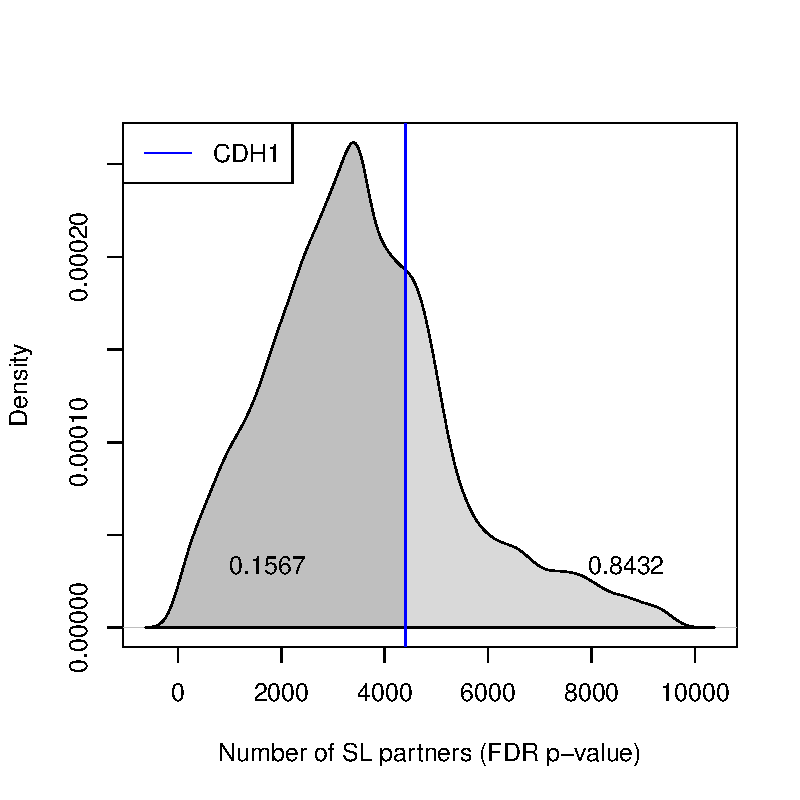
\includegraphics{MostSL_Summary_CDH1_FDR_stad.pdf}
   }
   \end{center}
   \caption[Synthetic lethal partners across query genes]{\small \textbf{Synthetic lethal partners across query genes.} Global synthetic lethal pairs were examined across the \glspl{genome} in \gls{TCGA} stomach expression data by applying SLIPT across query genes. The high number of predicted partners for \textit{CDH1} was typical for a human gene and lower than many other genes.
   }
\label{fig:global_SL_stad}
%\end{mdframed}
\end{figure*}


\FloatBarrier

\clearpage

\section{Hub Genes}


\begin{table*}[!ht]
\caption{Query synthetic lethal genes with the most SLIPT partners}
\label{tab:gene_mostSL_stad}
\centering
\resizebox{0.8 \textwidth}{!}{
\begin{threeparttable}
\begin{tabular}{>{\em}sl^c^c^c^c^c}
\hline
\rowstyle{\bfseries}
  \em{Gene} & Direction & raw p-value & p-value (\gls{FDR}) & SLIPT raw p-value & SLIPT (\gls{FDR}) \\ 
  \hline
  \rowcolor{black!10}
  HEG1 & 10719 & 16956 & 16724 & 9616 & 9532 \\ 
  \rowcolor{black!5}
  SYNE1 & 10755 & 17210 & 16984 & 9749 & 9676 \\ 
  \rowcolor{black!10}
  A2M & 10743 & 16650 & 16378 & 9529 & 9433 \\ 
  \rowcolor{black!5}
  ANK2 & 11008 & 16616 & 16355 & 9764 & 9653 \\ 
  \rowcolor{black!10}
  TTC28 & 10757 & 16523 & 16248 & 9530 & 9429 \\ 
  \rowcolor{black!5}
  FAT4 & 10451 & 16286 & 15978 & 9225 & 9115 \\ 
  \rowcolor{black!10}
  MRVI1 & 10904 & 16967 & 16718 & 9775 & 9686 \\ 
  \rowcolor{black!5}
  PAPLN & 10483 & 16405 & 16104 & 9305 & 9193 \\ 
  \rowcolor{black!10}
  NFASC & 10773 & 16575 & 16307 & 9578 & 9475 \\ 
  \rowcolor{black!5}
  MACF1 & 9697 & 16378 & 16058 & 8620 & 8540 \\ 
  \rowcolor{black!10}
  HMCN1 & 10475 & 16101 & 15733 & 9156 & 9008 \\ 
  \rowcolor{black!5}
  MPDZ & 10878 & 16550 & 16299 & 9599 & 9491 \\ 
  \rowcolor{black!10}
  FLRT2 & 10776 & 16760 & 16473 & 9590 & 9464 \\ 
  \rowcolor{black!5}
  SETBP1 & 10869 & 16632 & 16349 & 9615 & 9489 \\ 
  \rowcolor{black!10}
  LAMA4 & 10463 & 16447 & 16121 & 9273 & 9151 \\ 
  \rowcolor{black!5}
  IL1R1 & 10611 & 16185 & 15803 & 9299 & 9174 \\ 
  \rowcolor{black!10}
  ABCA6 & 10499 & 16573 & 16318 & 9260 & 9158 \\ 
  \rowcolor{black!5}
  LAMC1 & 10238 & 15777 & 15392 & 8837 & 8691 \\ 
  \rowcolor{black!10}
  TNS1 & 10920 & 17038 & 16806 & 9836 & 9751 \\ 
  \rowcolor{black!5}
  AMOTL1 & 10612 & 16458 & 16178 & 9367 & 9250 \\ 
  \hline
\end{tabular}
\begin{tablenotes}
\raggedright \small
Genes with the most candidate \gls{synthetic lethal} partners SLIPT in \gls{TCGA} stomach expression data with the number of partner genes predicted by direction criteria and $\chi^2$ testing separately and combined as a \gls{SLIPT} analysis. Where specified, the p-values for the $\chi^2$ test were adjusted for multiple tests (\gls{FDR}).
\end{tablenotes}
\end{threeparttable}
}
\end{table*}


\FloatBarrier

\clearpage

\section{Hub Pathways}

\begin{table*}[!ht]
\caption{Pathways for genes with the most SLIPT partners}
\label{tab:pathway_mostSL_stad}
\centering
\resizebox{1 \textwidth}{!}{
\begin{threeparttable}
\begin{tabular}{lcccc}
  \cellcolor{white} \textbf{Pathways Over-represented} & \textbf{Pathway Size} & \textbf{SL Genes} & \textbf{p-value} & \textbf{p-value (\gls{FDR})} \\
  \hline
  \rowcolor{black!10}
  Molecules associated with elastic fibres &  34 &  10 & $4.6 \times 10^{-21}$ & $2.7 \times 10^{-18}$ \\ 
  \rowcolor{black!5}
  Extracellular matrix organization & 241 &  29 & $5.3 \times 10^{-21}$ & $2.7 \times 10^{-18}$ \\ 
  \rowcolor{black!10}
  Smooth Muscle Contraction &  29 &   9 & $5.6 \times 10^{-20}$ & $1.6 \times 10^{-17}$ \\ 
  \rowcolor{black!5}
  Elastic fibre formation &  38 &  10 & $6 \times 10^{-20}$ & $1.6 \times 10^{-17}$ \\ 
  \rowcolor{black!10}
  Nitric oxide stimulates guanylate cyclase &  24 &   8 & $6.9 \times 10^{-19}$ & $1.4 \times 10^{-16}$ \\ 
  \rowcolor{black!5}
  Muscle contraction &  64 &  12 & $8.3 \times 10^{-19}$ & $1.4 \times 10^{-16}$ \\ 
  \rowcolor{black!10}
  Platelet homeostasis &  54 &  11 & $1.3 \times 10^{-18}$ & $1.9 \times 10^{-16}$ \\ 
  \rowcolor{black!5}
  cGMP effects &  18 &   6 & $3.3 \times 10^{-15}$ & $4.3 \times 10^{-13}$ \\ 
  \rowcolor{black!10}
  Laminin interactions &  30 &   7 & $1.3 \times 10^{-14}$ & $1.6 \times 10^{-12}$ \\ 
  \rowcolor{black!5}
  Axon guidance & 289 &  25 & $5 \times 10^{-13}$ & $5.2 \times 10^{-11}$ \\ 
  \rowcolor{black!10}
  Signalling by BMP &  23 &   5 & $3.7 \times 10^{-11}$ & $3.2 \times 10^{-9}$ \\ 
  \rowcolor{black!5}
  RHO GTPases activate PAKs &  23 &   5 & $3.7 \times 10^{-11}$ & $3.2 \times 10^{-9}$ \\ 
  \rowcolor{black!10}
  Non-integrin membrane-ECM interactions &  53 &   7 & $7.2 \times 10^{-11}$ & $5.8 \times 10^{-9}$ \\ 
  \rowcolor{black!5}
  Rho GTPase cycle & 120 &  11 & $1.2 \times 10^{-10}$ & $8.7 \times 10^{-9}$ \\ 
  \rowcolor{black!10}
  Degradation of the extracellular matrix & 104 &  10 & $1.3 \times 10^{-10}$ & $8.8 \times 10^{-9}$ \\ 
  \rowcolor{black!5}
  Netrin-1 signalling &  42 &   6 & $2.5 \times 10^{-10}$ & $1.6 \times 10^{-8}$ \\ 
  \rowcolor{black!10}
  Developmental Biology & 432 &  32 & $8.3 \times 10^{-10}$ & $5 \times 10^{-8}$ \\ 
  \rowcolor{black!5}
  L1CAM interactions &  80 &   8 & $8.7 \times 10^{-10}$ & $5 \times 10^{-8}$ \\ 
  \rowcolor{black!10}
  Semaphorin interactions &  64 &   7 & $1.1 \times 10^{-9}$ & $6.1 \times 10^{-8}$ \\ 
  \rowcolor{black!5}
  Cell-extracellular matrix interactions &  18 &   4 & $1.3 \times 10^{-9}$ & $6.6 \times 10^{-8}$ \\ 
   \hline
\end{tabular}
\begin{tablenotes}
\raggedright \small
Gene set over-representation analysis (hypergeometric test) for Reactome pathways in the top 500 ``hub'' genes with the most candidate synthetic lethal partners by \gls{SLIPT} analysis of \gls{TCGA} stomach expression data.
\end{tablenotes}
\end{threeparttable}
}
\end{table*}

\FloatBarrier

\iffalse
\chapter{Replication in cell line encyclopaedia} \label{appendix:CCLE}


\begin{table*}[!ht]
\caption{Candidate synthetic lethal gene partners of \textit{CDH1} from SLIPT in CCLE}
\label{tab:gene_ccle_SL}
\centering
\resizebox{0.8 \textwidth}{!}{
\begin{threeparttable}
\begin{tabular}{>{\em}sl^c^c^c^c^c}
\rowstyle{\bfseries}
 \em{Gene} & Observed & Expected & $\chi^2$ value & p-value & p-value (\gls{FDR}) \\ 
  \hline
  \rowcolor{black!10}
  ZEB1 & 24 & 115 & 555 & $7.84 \times 10^{-119}$ & $3.62 \times 10^{-116}$ \\ 
  \rowcolor{black!5}
  RP11-620J15.3 & 17 & 115 & 471 & $1.54 \times 10^{-100}$ & $3.68 \times 10^{-98}$ \\ 
  \rowcolor{black!10}
  AP1S2 & 20 & 115 & 462 & $1.38 \times 10^{-98}$ & $3.07 \times 10^{-96}$ \\ 
  \rowcolor{black!5}
  VIM & 24 & 115 & 424 & $1.73 \times 10^{-90}$ & $3.06 \times 10^{-88}$ \\ 
  \rowcolor{black!10}
  CCDC88A & 24 & 115 & 418 & $3.94 \times 10^{-89}$ & $6.86 \times 10^{-87}$ \\ 
  \rowcolor{black!5}
  RECK & 28 & 115 & 416 & $8.23 \times 10^{-89}$ & $1.42 \times 10^{-86}$ \\ 
  \rowcolor{black!10}
  AP1M1 & 16 & 115 & 414 & $2.42 \times 10^{-88}$ & $4.06 \times 10^{-86}$ \\ 
  \rowcolor{black!5}
  ZEB2 & 23 & 115 & 396 & $2.32 \times 10^{-84}$ & $3.4 \times 10^{-82}$ \\ 
  \rowcolor{black!10}
  WIPF1 & 25 & 115 & 390 & $4.9 \times 10^{-83}$ & $6.74 \times 10^{-81}$ \\ 
  \rowcolor{black!5}
  SLC35B4 & 29 & 115 & 386 & $3.2 \times 10^{-82}$ & $4.38 \times 10^{-80}$ \\ 
  \rowcolor{black!10}
  SACS & 28 & 115 & 373 & $2.13 \times 10^{-79}$ & $2.7 \times 10^{-77}$ \\ 
  \rowcolor{black!5}
  ST3GAL2 & 25 & 115 & 351 & $9.7 \times 10^{-75}$ & $1.08 \times 10^{-72}$ \\ 
  \rowcolor{black!10}
  ATP8B2 & 38 & 115 & 341 & $1.53 \times 10^{-72}$ & $1.61 \times 10^{-70}$ \\ 
  \rowcolor{black!5}
  IFFO1 & 39 & 115 & 332 & $1.66 \times 10^{-70}$ & $1.65 \times 10^{-68}$ \\ 
  \rowcolor{black!10}
  EMP3 & 38 & 115 & 329 & $5.04 \times 10^{-70}$ & $4.95 \times 10^{-68}$ \\ 
  \rowcolor{black!5}
  LEPRE1 & 40 & 115 & 325 & $5.4 \times 10^{-69}$ & $5.22 \times 10^{-67}$ \\ 
  \rowcolor{black!10}
  STARD9 & 39 & 115 & 311 & $4.52 \times 10^{-66}$ & $3.96 \times 10^{-64}$ \\ 
  \rowcolor{black!5}
  DENND5A & 48 & 115 & 304 & $1.89 \times 10^{-64}$ & $1.59 \times 10^{-62}$ \\ 
  \rowcolor{black!10}
  SYT11 & 38 & 115 & 300 & $1.21 \times 10^{-63}$ & $9.89 \times 10^{-62}$ \\ 
  \rowcolor{black!5}
  EID2B & 38 & 115 & 299 & $1.99 \times 10^{-63}$ & $1.61 \times 10^{-61}$ \\ 
  \rowcolor{black!10}
  NXPE3 & 35 & 115 & 294 & $1.71 \times 10^{-62}$ & $1.35 \times 10^{-60}$ \\ 
  \rowcolor{black!5}
  STX2 & 49 & 115 & 293 & $3.83 \times 10^{-62}$ & $3 \times 10^{-60}$ \\ 
  \rowcolor{black!10}
  ARHGEF6 & 43 & 115 & 289 & $2.2 \times 10^{-61}$ & $1.71 \times 10^{-59}$ \\ 
  \rowcolor{black!5}
  KATNAL1 & 50 & 115 & 283 & $4.45 \times 10^{-60}$ & $3.38 \times 10^{-58}$ \\ 
  \rowcolor{black!10}
  ANXA6 & 37 & 115 & 282 & $8.92 \times 10^{-60}$ & $6.67 \times 10^{-58}$ \\ 
  \hline
\end{tabular}
\begin{tablenotes}
\raggedright \small
Strongest candidate \gls{synthetic lethal} partners for \textit{CDH1} by SLIPT with observed and expected numbers of \gls{CCLE} samples with low expression of both genes.
\end{tablenotes}
\end{threeparttable}
}
\end{table*}


\begin{table*}[!ht]
\caption{Candidate synthetic lethal gene partners of \textit{CDH1} from SLIPT in breast CCLE}
\label{tab:gene_ccle_brca_SL}
\centering
\resizebox{0.8 \textwidth}{!}{
\begin{threeparttable}
\begin{tabular}{>{\em}sl^c^c^c^c^c}
\rowstyle{\bfseries}
 \em{Gene} & Observed & Expected & $\chi^2$ value & p-value & p-value (\gls{FDR}) \\ 
  \hline
  \rowcolor{black!10}
  MIR155HG & 1 & 6.78 & 31.5 & $2.41 \times 10^{-6}$ & 0.00371 \\ 
  \rowcolor{black!5}
  ENPP2 & 1 & 6.78 & 30.7 & $3.47 \times 10^{-6}$ & 0.00383 \\ 
  \rowcolor{black!10}
  DCLK2 & 3 & 6.78 & 28.3 & $1.08 \times 10^{-5}$ & 0.0071 \\ 
  \rowcolor{black!5}
  PID1 & 1 & 6.78 & 27.8 & $1.34 \times 10^{-5}$ & 0.00791 \\ 
  \rowcolor{black!10}
  SCFD2 & 5 & 6.78 & 27.7 & $1.42 \times 10^{-5}$ & 0.00791 \\ 
  \rowcolor{black!5}
  FAT4 & 4 & 6.78 & 27.3 & $1.69 \times 10^{-5}$ & 0.00865 \\ 
  \rowcolor{black!10}
  ILK & 1 & 6.78 & 26.9 & $2.04 \times 10^{-5}$ & 0.00884 \\ 
  \rowcolor{black!5}
  RWDD1 & 0 & 6.78 & 26.8 & $2.15 \times 10^{-5}$ & 0.00884 \\ 
  \rowcolor{black!10}
  RIC8A & 2 & 6.78 & 26.8 & $2.2 \times 10^{-5}$ & 0.00884 \\ 
  \rowcolor{black!5}
  F2RL2 & 1 & 6.78 & 26.6 & $2.34 \times 10^{-5}$ & 0.00901 \\ 
  \rowcolor{black!10}
  SDCBP & 5 & 6.78 & 25.9 & $3.26 \times 10^{-5}$ & 0.0108 \\ 
  \rowcolor{black!5}
  PPM1F & 4 & 6.78 & 25.8 & $3.41 \times 10^{-5}$ & 0.0108 \\ 
  \rowcolor{black!10}
  IKBIP & 5 & 6.78 & 25.8 & $3.49 \times 10^{-5}$ & 0.0108 \\ 
  \rowcolor{black!5}
  SPRED1 & 3 & 6.78 & 25.5 & $3.97 \times 10^{-5}$ & 0.0108 \\ 
  \rowcolor{black!10}
  RNH1 & 1 & 6.78 & 25.4 & $4.22 \times 10^{-5}$ & 0.0108 \\ 
  \rowcolor{black!5}
  SYDE1 & 3 & 6.78 & 25.4 & $4.22 \times 10^{-5}$ & 0.0108 \\ 
  \rowcolor{black!10}
  LINC00968 & 1 & 6.78 & 25.2 & $4.63 \times 10^{-5}$ & 0.0109 \\ 
  \rowcolor{black!5}
  ARHGEF10 & 5 & 6.78 & 24.5 & $6.22 \times 10^{-5}$ & 0.0116 \\ 
  \rowcolor{black!10}
  P4HA1 & 0 & 6.78 & 24.5 & $6.34 \times 10^{-5}$ & 0.0116 \\ 
  \rowcolor{black!5}
  AZI2 & 2 & 6.78 & 24.5 & $6.34 \times 10^{-5}$ & 0.0116 \\ 
  \rowcolor{black!10}
  TNFAIP6 & 2 & 6.78 & 24.5 & $6.34 \times 10^{-5}$ & 0.0116 \\ 
  \rowcolor{black!5}
  CD200 & 4 & 6.78 & 24.5 & $6.37 \times 10^{-5}$ & 0.0116 \\ 
  \rowcolor{black!10}
  SMPD1 & 1 & 6.78 & 24.4 & $6.67 \times 10^{-5}$ & 0.0116 \\ 
  \rowcolor{black!5}
  ATP6V1G2 & 3 & 6.78 & 24.2 & $7.33 \times 10^{-5}$ & 0.0123 \\ 
  \rowcolor{black!10}
  FGF2 & 4 & 6.78 & 24.1 & $7.49 \times 10^{-5}$ & 0.0123 \\ 
  \hline
\end{tabular}
\begin{tablenotes}
\raggedright \small
Strongest candidate \gls{synthetic lethal} partners for \textit{CDH1} by SLIPT with observed and expected numbers of \gls{CCLE} breast samples with low expression of both genes.
\end{tablenotes}
\end{threeparttable}
}
\end{table*}

\begin{table*}[!ht]
\caption{Candidate synthetic lethal gene partners of \textit{CDH1} from SLIPT in stomach CCLE}
\label{tab:gene_ccle_stad_SL}
\centering
\resizebox{0.8 \textwidth}{!}{
\begin{threeparttable}
\begin{tabular}{>{\em}sl^c^c^c^c^c}
\rowstyle{\bfseries}
 \em{Gene} & Observed & Expected & $\chi^2$ value & $p-value$ & p-value (\gls{FDR}) \\ 
  \hline
  \rowcolor{black!10}
  ZEB1 & 1 & 4.45 & 36 & $2.84 \times 10^{-7}$ & 0.00175 \\ 
  \rowcolor{black!5}
  WDR47 & 0 & 4.45 & 26.7 & $2.3 \times 10^{-5}$ & 0.013 \\ 
  \rowcolor{black!10}
  KANK2 & 1 & 4.45 & 25.1 & $4.81 \times 10^{-5}$ & 0.0222 \\ 
  \rowcolor{black!5}
  LEPRE1 & 0 & 4.45 & 24.5 & $6.26 \times 10^{-5}$ & 0.0228 \\ 
  \rowcolor{black!10}
  KATNAL1 & 0 & 4.45 & 24.3 & $6.88 \times 10^{-5}$ & 0.0231 \\ 
  \rowcolor{black!5}
  TET1 & 0 & 4.45 & 23.9 & $8.23 \times 10^{-5}$ & 0.0249 \\ 
  \rowcolor{black!10}
  AP1S2 & 1 & 4.45 & 23.1 & $0.00012$ & 0.0273 \\ 
  \rowcolor{black!5}
  CDKN2C & 1 & 4.45 & 22.8 & $0.000136$ & 0.0292 \\ 
  \rowcolor{black!10}
  ARMC4 & 1 & 4.45 & 22.4 & $0.000164$ & 0.0315 \\ 
  \rowcolor{black!5}
  CSTF3 & 1 & 4.45 & 22.4 & $0.000166$ & 0.0315 \\ 
  \rowcolor{black!10}
  FAM216A & 1 & 4.45 & 22.4 & $0.000166$ & 0.0315 \\ 
  \rowcolor{black!5}
  ANKRD32 & 1 & 4.45 & 22.4 & $0.000166$ & 0.0315 \\ 
  \rowcolor{black!10}
  WDR35 & 1 & 4.45 & 22.4 & $0.000169$ & 0.0315 \\ 
  \rowcolor{black!5}
  ECI2 & 0 & 4.45 & 21.7 & $0.000232$ & 0.0378 \\ 
  \rowcolor{black!10}
  SAMD8 & 0 & 4.45 & 21.7 & $0.000232$ & 0.0378 \\ 
  \rowcolor{black!5}
  CHST12 & 0 & 4.45 & 21.7 & $0.000232$ & 0.0378 \\ 
  \rowcolor{black!10}
  RPL23AP32 & 0 & 4.45 & 21.7 & $0.000232$ & 0.0378 \\ 
  \rowcolor{black!5}
  STARD9 & 1 & 4.45 & 21.7 & $0.000232$ & 0.0378 \\ 
  \rowcolor{black!10}
  MCM8 & 0 & 4.45 & 21.5 & $0.000255$ & 0.0379 \\ 
  \hline
\end{tabular}
\begin{tablenotes}
\raggedright \small
Strongest candidate \gls{synthetic lethal} partners for \textit{CDH1} by SLIPT with observed and expected numbers of \gls{CCLE} stomach samples with low expression of both genes.
\end{tablenotes}
\end{threeparttable}
}
\end{table*}



\begin{table*}[!ht]
\caption{Pathways for \textit{CDH1} partners from SLIPT in stomach CCLE}
\label{tab:pathway_ccle_stad_exprSL}
\centering
\resizebox{1 \textwidth}{!}{
\begin{threeparttable}
\begin{tabular}{lccc}
  \hline
  \cellcolor{white} \textbf{Pathways Over-represented} & \textbf{Pathway Size} & \textbf{SL Genes} & \textbf{p-value (\gls{FDR})} \\
  \hline
  \rowcolor{black!10}
  Nef mediated downregulation of MHC class I complex cell surface expression &  10 &   1 &   1 \\ 
  \rowcolor{black!5}
  Unwinding of \acrshort{DNA} &  11 &   1 &   1 \\ 
  \rowcolor{black!10}
  Processing of Intronless Pre-mRNAs &  13 &   1 &   1 \\ 
  \rowcolor{black!5}
  E2F mediated regulation of \acrshort{DNA} replication &  20 &   1 &   1 \\ 
  \rowcolor{black!10}
  Chondroitin sulfate biosynthesis &  20 &   1 &   1 \\ 
  \rowcolor{black!5}
  Post-Elongation Processing of Intronless pre-mRNA &  21 &   1 &   1 \\ 
  \rowcolor{black!10}
 \begin{tabular}[c]{@{}l@{}} Nef-mediates down modulation of cell surface receptors by recruiting them \\ to clathrin adapters \end{tabular} &  21 &   1 &   1 \\ 
  \rowcolor{black!5}
  Processing of Capped Intronless Pre-mRNA &  21 &   1 &   1 \\ 
  \rowcolor{black!10}
  Post-Elongation Processing of Intron-Containing pre-mRNA &  23 &   1 &   1 \\ 
  \rowcolor{black!5}
  Activation of the pre-replicative complex &  23 &   1 &   1 \\ 
  \rowcolor{black!10}
  \acrshort{mRNA} 3'-end processing &  23 &   1 &   1 \\ 
  \rowcolor{black!5}
  Golgi Associated Vesicle Biogenesis &  24 &   1 &   1 \\ 
  \rowcolor{black!10}
  Lysosome Vesicle Biogenesis &  25 &   1 &   1 \\ 
  \rowcolor{black!5}
  Oncogene Induced Senescence &  27 &   1 &   1 \\ 
  \rowcolor{black!10}
  The role of Nef in HIV-1 replication and disease pathogenesis &  28 &   1 &   1 \\ 
  \rowcolor{black!5}
  Cyclin D associated events in G1 &  29 &   1 &   1 \\ 
  \rowcolor{black!10}
  G1 Phase &  29 &   1 &   1 \\ 
  \rowcolor{black!5}
  Cleavage of Growing Transcript in the Termination Region &  31 &   1 &   1 \\ 
  \rowcolor{black!10}
  Activation of ATR in response to replication stress &  31 &   1 &   1 \\ 
  \rowcolor{black!5}
  \acrshort{DNA} strand elongation &  31 &   1 &   1 \\ 
  \rowcolor{black!10}
  \hline
\end{tabular}
\begin{tablenotes}
\raggedright \small
Gene set over-representation analysis (hypergeometric test) for Reactome pathways in SLIPT partners for \textit{CDH1}.
\end{tablenotes}
\end{threeparttable}
}
\end{table*}


\begin{table*}[!ht]
\caption{Pathways for \textit{CDH1} partners from SLIPT in breast and stomach CCLE}
\label{tab:pathway_ccle_breast_stad_exprSL}
\centering
\resizebox{1 \textwidth}{!}{
\begin{threeparttable}
\begin{tabular}{lccc}
  \hline
  \cellcolor{white} \textbf{Pathways Over-represented} & \textbf{Pathway Size} & \textbf{SL Genes} & \textbf{p-value (\gls{FDR})} \\
  \hline
  \rowcolor{black!10}
  Collagen formation &  66 &   8 &  $1.1 \times 10^{-7}$ \\ 
  \rowcolor{black!5}
  Glycosaminoglycan metabolism & 111 &  11 & $1.1 \times 10^{-7}$ \\ 
  \rowcolor{black!10}
  Extracellular matrix organization & 236 &  20 & $1.1 \times 10^{-7}$ \\ 
  \rowcolor{black!5}
  Collagen biosynthesis and modifying enzymes &  55 &   7 & $1.7 \times 10^{-7}$ \\ 
  \rowcolor{black!10}
  Keratan sulfate biosynthesis &  28 &   5 & $2.2 \times 10^{-7}$ \\ 
  \rowcolor{black!5}
  Keratan sulfate/keratin metabolism &  32 &   5 & $7.5 \times 10^{-7}$ \\ 
  \rowcolor{black!10}
  ECM proteoglycans &  65 &   7 & $1.1 \times 10^{-6}$ \\ 
  \rowcolor{black!5}
  Non-integrin membrane-ECM interactions &  52 &   6 & $2.0 \times 10^{-6}$ \\ 
  \rowcolor{black!10}
  Cell junction organization &  71 &   7 & $3.0 \times 10^{-6}$ \\ 
  \rowcolor{black!5}
  Assembly of collagen fibrils and other multimeric structures &  39 &   5 & $3.6 \times 10^{-6}$ \\ 
  \rowcolor{black!10}
  Post-chaperonin tubulin folding pathway &  14 &   3 & $1.7 \times 10^{-5}$ \\ 
  \rowcolor{black!5}
  Adherens junctions interactions &  29 &   4 & $1.7 \times 10^{-5}$ \\ 
  \rowcolor{black!10}
  Cell-Cell communication & 118 &   9 & $1.7 \times 10^{-5}$ \\ 
  \rowcolor{black!5}
  Sialic acid metabolism &  31 &   4 & $2.5 \times 10^{-5}$ \\ 
  \rowcolor{black!10}
  Synthesis and interconversion of nucleotide di- and triphosphates &  16 &   3 & $3.1 \times 10^{-5}$ \\ 
  \rowcolor{black!5}
  Transport to the Golgi and subsequent modification &  34 &   4 & $4.8 \times 10^{-5}$ \\ 
  \rowcolor{black!10}
  Asparagine N-linked glycosylation & 113 &   8 & $7.8 \times 10^{-5}$ \\ 
  \rowcolor{black!5}
  Elastic fibre formation &  37 &   4 & $8.5 \times 10^{-5}$ \\ 
  \rowcolor{black!10}
  L1CAM interactions &  77 &   6 & $9.5 \times 10^{-5}$ \\ 
  \rowcolor{black!5}
  Signal transduction by L1 &  20 &   3 & $9.5 \times 10^{-5}$ \\ 
  \hline
\end{tabular}
\begin{tablenotes}
\raggedright \small
Gene set over-representation analysis (hypergeometric test) for Reactome pathways in SLIPT partners for \textit{CDH1}.
\end{tablenotes}
\end{threeparttable}
}
\end{table*}

\FloatBarrier
\fi